\documentclass[12pt]{article}
 
\usepackage[margin=1in]{geometry} 
\usepackage{amsmath,amsthm,amssymb,graphicx,mathtools,tikz,float,mathrsfs,multicol,textcomp,gensymb,extarrows,dsfont,tikz-cd,subcaption,enumerate,cancel}
\usepackage[urlcolor=blue]{hyperref}
\hypersetup{
     colorlinks   = true,
     citecolor    = gray
} % Lime green, really?! Not only is that a sore sight, lime green has been an enemy of mine since 2007.
\usetikzlibrary{positioning}
\newcommand{\n}{\mathbb{N}}
\newcommand{\z}{\mathbb{Z}}
\newcommand{\q}{\mathbb{Q}}
\newcommand{\cx}{\mathbb{C}}
\newcommand{\real}{\mathbb{R}}
\newcommand{\field}{\mathbb{F}}
\newcommand{\h}{\mathbb{H}}
\newcommand{\m}{\mathbb{M}}
\newcommand{\p}{\mathbb{P}}
\newcommand{\ita}[1]{\textit{#1}}
\newcommand{\oneton}[1]{\{1,\dotsc,#1\}}
\newcommand\idea[1]{\begin{gather*}#1\end{gather*}}
\newcommand\proofs[1]{\begin{proof}#1\end{proof}}
\newcommand\inv[1]{#1^{-1}}
\newcommand\paren[1]{\left( #1 \right)}
\newcommand\setb[1]{\left \{ #1 \right \}}
\newcommand{\sqbrack}[1]{\left [ #1 \right ]}
\newcommand{\vbrack}[1]{\left \langle #1 \right \rangle}
\newcommand{\abs}[1]{\left| #1 \right|}
\newcommand{\norm}[1]{\left\| #1 \right\|}
\newcommand{\eps}{\varepsilon}
\newcommand{\ds}{\displaystyle}
\renewcommand{\i}[4]{\int_{#1}^{#2} {#3} \, \mathrm{d} {#4} }
\newcommand{\mono}{\hookrightarrow}
\newcommand{\epi}{\twoheadrightarrow}
\newcommand{\rd}{\mathrm{d}}
\newcommand{\Nabla}{\boldsymbol{\nabla}}
\newcommand{\fl}[1]{\left \lfloor #1 \right \rfloor}
\newcommand{\cl}[1]{\left \lceil #1 \right \rceil}

\newtheorem{theorem}{Theorem}[section]
\newtheorem{corollary}{Corollary}[theorem]
\newtheorem{lemma}[theorem]{Lemma}
\newtheorem*{claim}{Claim}
\theoremstyle{definition}
\newtheorem{definition}{Definition}[section]
\newtheorem*{remark}{Remark}

\hypersetup{
 colorlinks,
 linkcolor=blue
}

\allowdisplaybreaks

\usepackage[shortlabels]{enumitem}

\DeclareMathOperator\Log{Log}
\DeclareMathOperator\Res{Res}
\DeclareMathOperator\re{Re}
\DeclareMathOperator\im{Im}

\begin{document}
\date{last updated 23 May 2022} 
\author{Alexander Louis J. Sabater}
\title{Complex Analysis}
\maketitle
\newpage 
\tableofcontents
\newpage
\begin{abstract}
    These are my attempted solutions to the complex analysis portion of the UC Santa Barbara Analysis qualifying exams, ordered by date. For more practice, I've also included some problems involving residues from \cite{Conway}. $\n$ denotes $\setb{ 0 } \cup \z^+$, $\cx^{\times}$ denotes $\cx \setminus \setb{ 0 }$ (thankfully this notation is consistent since $\cx$ is a field), $B(a;r)$ denotes the open ball of radius $r$ centered at $a$, $\bar{B}(a;r)$ denotes the closed ball of radius $r$ centered at $a$ (and thankfully since $\cx$ is a real normed vector space this is equal to the closure of $B(a;r)$), $n(\gamma;a)$ denotes the winding number of $\gamma$ around the point $a$, and $\Res(f;a)$ denotes the residue of $f$ at $a$. A completed qual means every question has been answered completely, an answered qual means enough questions have been answered to turn in.
\end{abstract}
\section{Spring 1992 [Completed]}
Do 5 problems in each section. State which problems in each section you are not doing.
\subsection{Problem 1 \texorpdfstring{\cite{Res}}{}}
Evaluate the integral 
\[
    \int_{-\infty}^{\infty} \frac{x^2 - 1}{(x^2+1)^2} \, \mathrm{d}x.
\]
\begin{proof}[Answer]
    If $f$ is a meromorphic function with a pole $z_0$ of order $m$, then 
    \begin{equation}\label{eq1}
        \Res(f;z_0) = \frac{1}{(m-1)!} \frac{\mathrm{d}^{m-1}}{\mathrm{d}z^{m-1}} \left. \sqbrack{ (z - z_0)^m f(z) } \right|_{z = z_0}.
    \end{equation}
    Let 
    \[
        f(z) \coloneqq \frac{z^2 - 1}{ \paren{ z^2 + 1 }^2 } = \frac{ z^2 - 1 }{ \paren{ z - i }^2 \paren{ z + i }^2 }.
    \]
    $f$ is meromorphic with poles at $z = \pm i$ of order 2. Let $R > 1$, and let $\gamma$ be the upper semicircle of radius $R$ centered a the origin, oriented counterclockwise.
    \begin{figure}[H]
        \centering
        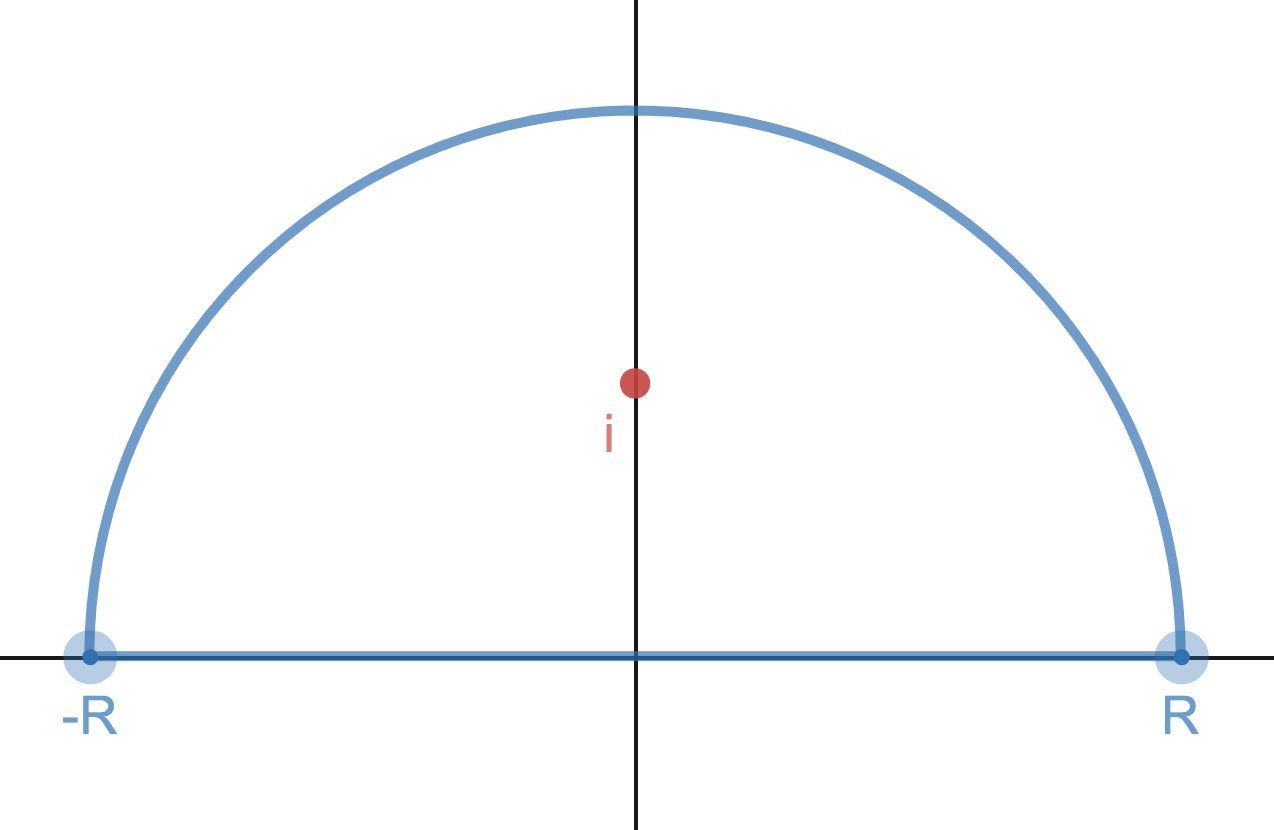
\includegraphics[width = 0.5\textwidth]{3.png}
        \caption{$\gamma$. Plotted in \cite{Desmos}.}
        \label{fig:fig1}
    \end{figure}
    Then by Residue Theorem,
    \[
        \int_{\gamma} f(z) \, \mathrm{d}z = 2\pi i \Res(f;i).
    \]
    Using \eqref{eq1}, 
    \begin{align*}
        \Res(f;i) & = \frac{1}{(2-1)!}  \frac{\mathrm{d}^{2-1}}{\mathrm{d}z^{2-1}} \left. \sqbrack{ (z - i)^2 f(z) } \right|_{z = i} = \frac{ \mathrm{d} }{ \mathrm{d}z } \left. \sqbrack{ \frac{ z^2 - 1 }{ (z + i)^2} } \right|_{z = i} \\[0.2em]
        & = \left. \frac{ (z + i)^2 (2z) - (z^2 - 1) 2(z + i) }{ (z + i)^4 } \right|_{z = i} = \frac{ (i + i)^2 (2i) - 2(i^2 - 1)(i + i)  }{ (2i)^4 } \\[0.2em]
        & = \frac{ (2i)^2 (2i) - 2(-1 -1)(2i) }{16} = \frac{-8i + 8i}{16} \\
        & = 0.
    \end{align*}
    Thus
    \begin{align*}
        0 & = \int_{\gamma} f(z) \, \mathrm{d}z = \int_{-R}^R \frac{x^2 - 1}{\paren{x^2+1}^2} \, \mathrm{d}x + \underbrace{ \int_0^{\pi} \frac{R^2 e^{2it} - 1}{ \paren{ R^2 e^{2it} + 1 }^2  } iR e^{it} \mathrm{d}t }_{ \eqqcolon I(R) } , \\
        -I(R) & = \int_{-R}^R \frac{x^2 - 1}{\paren{x^2+1}^2} \, \mathrm{d}x .
    \end{align*}
    Note that 
    \begin{align*}
        0 & \leq |I(R)| = \left| iR \int_0^{\pi} \frac {e^{it} \paren{ R^2 e^{2it} - 1 } }{ \paren{ R^2 e^{2it} + 1 }^2 } \, \mathrm{d} t \right| \leq R \int_0^{\pi} \frac{ \left| R^2 e^{2it} - 1 \right| }{ \left| R^2 e^{2it} + 1 \right|^2 } \, \mathrm{d} t.
    \end{align*}
    For all $0 \leq t \leq \pi$, 
    \[
        \left| R^2 e^{2it} - 1 \right| \leq \left| R^2 e^{2it} \right| + |-1| = R^2 + 1,
    \]
    and 
    \begin{align*}
        \left| R^2 e^{2it} + 1 - 1 \right| & \leq \left| R^2 e^{2it} + 1 \right| + | -1 | \\
        \left| R^2 e^{2it} \right| & \leq \left| R^2 e^{2it} + 1 \right| + 1 \\
        \Rightarrow \abs{ R^2 e^{2it} + 1 } & \geq R^2 - 1.
    \end{align*}
    Thus 
    \begin{align*}
        0 & \leq |I(R)| \leq R \int_0^{\pi} \frac{R^2 + 1}{ \paren{ R^2 - 1 }^2 } \, \mathrm{d}t \\
        & = \frac{ \pi R \paren{ R^2 + 1 } }{ \paren{ R^2 - 1 }^2 } \to 0
    \end{align*}
    as $R \to \infty$. Thus 
    \begin{align*}
        \int_{-\infty}^{+\infty} \frac{x^2 - 1}{(x^2+1)^2} \, \mathrm{d}x & = \lim\limits_{R \to \infty} \sqbrack{ \int_{-R}^R \frac{x^2 - 1}{\paren{x^2+1}^2} \, \mathrm{d}x } = \lim\limits_{R \to \infty} -I(R) = \boxed{ 0. }
    \end{align*}
    Note that this integral can also be computed with real variable methods. Let $x = \tan \theta$, then $ -\frac{\pi}{2} \leq x \leq \frac{\pi}{2}$ and $\mathrm{d} x = \sec^2 \theta \, \mathrm{d}\theta$. Thus 
    \begin{align*}
        I & \coloneqq \int_{-\infty}^{+\infty} \frac{x^2 - 1}{(x^2+1)^2} \, \mathrm{d}x = \int_{-\frac{\pi}{2}}^{\frac{\pi}{2}} \frac{ \tan^2 \theta - 1 }{ \paren{ \tan^2 \theta + 1 }^2 } \sec^2 \theta \, \mathrm{d} \theta.
    \end{align*}
    Using $\tan^2 \theta + 1 = \sec^2 \theta$, 
    \begin{align*}
        I & = \int_{-\frac{\pi}{2}}^{\frac{\pi}{2}} \frac{ \tan^2 \theta - 1 }{ \paren{ \sec^2 \theta }^2 } \sec^2 \theta \, \mathrm{d} \theta = \int_{-\frac{\pi}{2}}^{\frac{\pi}{2}} \frac{ \tan^2 \theta - 1 }{ \sec^2 \theta } \, \mathrm{d}\theta \\
        & = \int_{-\frac{\pi}{2}}^{\frac{\pi}{2}} \paren{ \cos^2 \theta \tan^2 \theta - \cos^2 \theta } \, \mathrm{d}\theta = \int_{-\frac{\pi}{2}}^{\frac{\pi}{2}} \paren{ \sin^2 \theta - \cos^2 \theta } \, \mathrm{d}\theta \\
        & = \int_{-\frac{\pi}{2}}^{\frac{\pi}{2}} \sqbrack{ \frac{1 - \cos(2\theta)}{2} - \frac{1 - \sin(2\theta)}{2} } \, \mathrm{d}\theta = \int_{-\frac{\pi}{2}}^{\frac{\pi}{2}} -2 \cos(2\theta) \, \mathrm{d}\theta \\
        & = \left. -\frac{1}{2} \sin(2\theta) \right|_{\theta = -\frac{\pi}{2}}^{\theta = \frac{\pi}{2}} = -\frac{1}{2} \sqbrack{ \sin(\pi) - \sin(-\pi) } \\
        & = \boxed{ 0. }
    \end{align*}
\end{proof}
\subsection{Problem 2}
Suppose $F$ is an analytic function which maps the region $\Omega$ onto the open unit disk, and $U$ is a harmonic function on the open unit disk. Show that the composition $W = U \circ F$ is harmonic on $\Omega$.
\begin{proof}[Answer]
    Let $\Omega \subseteq \cx$ be open and connected, and let $F : \Omega \to D$ be analytic, $U : D \to \cx$ be harmonic. Write $F(x + iy) = f(x,y) + i g(x,y)$, $U(x + iy) = u(x,y) + i v(x,y)$, then
    \begin{align*}
        u_{xx}(x,y) + u_{yy}(x,y) & = 0, \\
        v_{xx}(x,y) + v_{yy}(x,y) & = 0,
    \end{align*}
    and by Cauchy-Riemann, 
    \begin{align*}
        f_{x}(x,y) & = g_{y}(x,y), \\
        f_{y}(x,y) & = -g_{x}(x,y).
    \end{align*}
    Furthermore, as $F$ is holomorphic, it is also harmonic, and so 
    \begin{align*}
        f_{xx}(x,y) + f_{yy}(x,y) & = 0, \\
        g_{xx}(x,y) + g_{yy}(x,y) & = 0.
    \end{align*}
    Then consider $W \coloneqq U \circ F : \Omega \to \cx $, given by 
    \[
        W(x + iy) = (U \circ F)(x + iy) = u \big( f(x,y) , g(x,y) \big) + i v \big( f(x,y) , g(x,y) \big).
    \]
    For convenience, we drop the arguments of the functions. Now, we compute the Laplacian of $W$:
    \begin{align*}
        W_x & = u_x ( f , g ) f_x + u_y ( f , g ) g_x + i \sqbrack{ v_x ( f , g ) f_x + v_y ( f , g ) g_x } , \\
        W_y & = u_x ( f , g ) f_y + u_y ( f , g ) g_y + i \sqbrack{ v_x ( f , g ) f_y + v_y ( f , g ) g_y } .
    \end{align*}
    Using Cauchy-Riemann, we rewrite the partials as (this time dropping the arguments of the partials of $u$ and $v$)
    \begin{align*}
        W_x & = u_x f_x - u_y f_y + i \paren{ v_x f_x - v_y f_y } , \\
        W_y & = u_x f_y + u_y f_x + i \paren{ v_x f_y + v_y f_x } .
    \end{align*}
    Then 
    \begin{align*}
        W_{xx} & = u_{xx} f_x + u_x f_{xx} - u_{yx} f_y - u_y f_{yx} \\
        & + i \paren{ v_{xx} f_x + v_x f_{xx} - v_{yx} f_y - v_y f_{yx} } \\
        W_{yy} & = u_{xy} f_y + u_x f_{yy} + u_{yy} f_x + u_y f_{xy} \\
        & + i \paren{ v_{xy} f_y + v_x f_{yy} + v_{yy} f_x + v_y f_{xy} }.
    \end{align*}
    Note that as $U$ and $F$ are harmonic, the mixed partials commute, so we can rewrite $W_{xx}$ as
    \begin{align*}
        W_{xx} & = u_{xx} f_x + u_x f_{xx} - u_{xy} f_y - u_y f_{xy} \\
        & + i \paren{ v_{xx} f_x + v_x f_{xx} - v_{xy} f_y - v_y f_{xy} }.
    \end{align*}
    Then finally
    \begin{align*}
        \re \paren{ W_{xx} + W_{yy} } & = u_{xx} f_x + u_x f_{xx} - u_{xy} f_y - u_y f_{xy} \\
        & + u_{xy} f_y + u_x f_{yy} + u_{yy} f_x + u_y f_{xy} \\ 
        & = u_{xx} f_x + u_x f_{xx} + u_x f_{yy} + u_{yy} f_x \\
        & = \paren{ u_{xx} + u_{yy} } \cdot f_x + u_x \cdot \paren{ f_{xx} + f_{yy} } \\
        & = 0, \\
        \im \paren{ W_{xx} + W_{yy} } & = v_{xx} f_x + v_x f_{xx} - v_{xy} f_y - v_y f_{xy} \\
        & + v_{xy} f_y + v_x f_{yy} + v_{yy} f_x + v_y f_{xy} \\
        & = v_{xx} f_x + v_x f_{xx} v_x f_{yy} + v_{yy} f_x \\
        & = \paren{ v_{xx} + v_{yy} } \cdot f_x + v_x \cdot \paren{ f_{xx} + f_{yy} } \\
        & = 0.
    \end{align*}
    Therefore $W = U \circ F$ is harmonic.
\end{proof}
\subsection{Problem 3}
\begin{enumerate}[i)]
    \item Find all the Laurent expansions of $h(z) = \frac{1}{z^2 (1-z)}$ about the origin.
    \item What is the residue of $h$ at the origin?
    \item What is the residue of $h$ at $z = 1$?
\end{enumerate}
\begin{proof}[Answer]
    \noindent
    \begin{enumerate}[i)]
        \item For $0 < |z| < 1$, we have
        \begin{align*}
            h(z) & = \frac{1}{z^2 (1-z)} = \frac{1}{z^2} \sum\limits_{n = 0}^{\infty} z^n = \frac{1}{z^2} + \frac{1}{z} + \sum\limits_{n = 0}^{\infty} z^n.
        \end{align*}
        Note that 
        \begin{align*}
            \frac{1}{z^2 (1-z)} & = \frac{1}{z^2} \frac{1}{z \paren{ \frac{1}{z} - 1 }} = -\frac{1}{z^3} \frac{1}{\paren{1 - \frac{1}{z} }} = -\frac{1}{z^3} \sum\limits_{n = 0}^{\infty} \paren{ \frac{1}{z} }^n = -\sum\limits_{n = 3}^{\infty} z^{-n}
        \end{align*}
        for $\left| \frac{1}{z} \right| < 1$, or equivalently for $|z| > 1$. Thus
        \begin{align*}
            h(z) = 
            \begin{cases}
                \frac{1}{z^2} + \frac{1}{z} + \sum\limits_{n = 0}^{\infty} z^n , & \quad |z| < 1 , \\
                -\sum\limits_{n = 3}^{\infty} z^{-n} , & \quad |z| > 1.
            \end{cases}
        \end{align*}
        \item Using the Laurent expansion for $0 < |z| < 1$, we have 
        \[
            \Res(h;0) = a_{-1} = \boxed{ 1. }
        \]
        \item Expand $h$ in partial fractions:
        \[
            h(z) = \frac{A}{z^2} + \frac{B}{z} + \frac{C}{1-z}
        \]
        for undetermined coefficients $A , B , C \in \cx$. Then 
        \begin{align*}
            1 & = z^2 (1-z) \\
            & = A(1-z) + Bz(1-z) + Cz^2 \\
            & = A - Az + Bz - Bz^2 + Cz^2 \\
            & = A + (B-A)z + (C-B)z^2.
        \end{align*}
        Thus $A = 1$, $B - A = 0$, and $C - B = 0$. This gives us $B = 1$, and $C = 1$, and so 
        \[
            h(z) = \frac{1}{z^2} + \frac{1}{z} + \frac{1}{1-z} = \frac{1}{z} \paren{ \frac{1}{z} + 1 } - (z-1)^{-1}.
        \]
        We expand $\frac{1}{z}$ about $z = 1$. First write 
        \[
            \frac{1}{z} = \frac{D}{1-E(z-1)}
        \]
        for some undetermined coefficients $D , E \in \cx$. Then 
        \[
            z = \frac{E+1}{D} - \frac{E}{D}z
        \]
        and so $\frac{E+1}{D} = 0$ and $-\frac{E}{D} = 1$. This gives us $E = -1$ and $D = 1$, so 
        \begin{align*}
            \frac{1}{z} & = \frac{1}{1 - \sqbrack{-1 (z-1)} } = \sum\limits_{n = 0}^{\infty} \sqbrack{ -(z-1) }^n = \sum\limits_{n = 0}^{\infty} (-1)^n (z-1)^n
        \end{align*}
        for $|(-1)(z-1)| = |z-1| < 1$. Thus the Laurent expansion of $\frac{1}{z}$, and in turn $\frac{1}{z^2} + \frac{1}{z}$, for $|z-1| < 1$ contains no negative powers. Hence the only negative power in the Laurent expansion of $h$ for $0<|z-1|<1$ is the $-(z-1)^{-1}$ term, thus
        \[
            \Res(h;1) = \boxed{ -1. }
        \]
    \end{enumerate}
\end{proof}
\subsection{Problem 4 \texorpdfstring{\cite{Elbow}}{}}
Suppose that $f$ is analytic except for isolated singularities at $+1$, $-1$, and $+i$, Given that 
\[
    \int_{\gamma_1} f \, \mathrm{d} z = 3 , \quad \int_{\gamma_2} f \, \mathrm{d} z = -1 , \quad \int_{\gamma_3} f \, \mathrm{d} z = -2,
\]
find the integral $\int_{\gamma} f \, \mathrm{d} z$.
\begin{figure}[H]
    \centering
    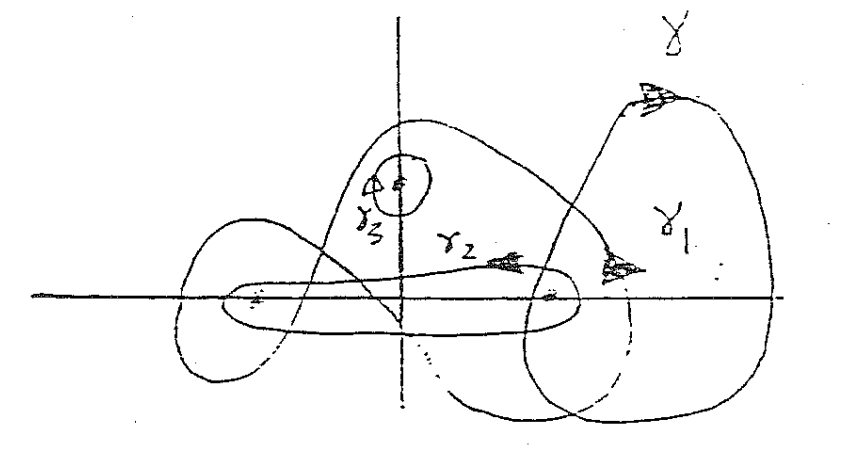
\includegraphics[width = 0.5\textwidth]{1.png}
    \caption{}
    \label{fig:fig2}
\end{figure}
\begin{proof}[Answer]
    By Reside Theorem,
    \begin{align*}
        3 & = \int_{\gamma_1} f(z) \, \mathrm{d}z = 2\pi i \sqbrack{ n(\gamma_1;1) \Res(f;1) + n(\gamma_1;-1) \Res(f;-1) + n(\gamma_1;i) \Res(f;i) } \\
        -1 & = \int_{\gamma_2} f(z) \, \mathrm{d}z = 2\pi i \sqbrack{ n(\gamma_2;1) \Res(f;1) + n(\gamma_2;-1) \Res(f;-1) } \\
        -2 & = \int_{\gamma_3} f(z) \, \mathrm{d}z = 2\pi i n(\gamma_3;i) \Res(f;i).
    \end{align*}
    Assume that each of the $\gamma_i$'s traverse once. Then
    \begin{align*}
        3 & = \int_{\gamma_1} f(z) \, \mathrm{d}z = 2\pi i \sqbrack{ \Res(f;1) - \Res(f;-1) + \Res(f;i) } \\
        -1 & = \int_{\gamma_2} f(z) \, \mathrm{d}z = 2\pi i \sqbrack{ \Res(f;1) + \Res(f;-1) } \\
        -2 & = \int_{\gamma_3} f(z) \, \mathrm{d}z = -2\pi i \Res(f;i),
    \end{align*}
    and so $\Res(f;i) = \frac{1}{\pi i}$. Letting $A \coloneqq \Res(f;1)$, $B \coloneqq \Res(f;-1)$, we have
    \begin{align*}
        3 & = 2\pi i \paren{ A - B + \frac{1}{\pi i} } \\
        & = 2\pi i ( A - B ) + 2 \\
        1 & = 2\pi i (A - B) \\
        -1 & = 2\pi i (A + B).
    \end{align*}
    Solving the system gives us $4 \pi A = 0$, or $A = 0$. Thus $B = -\frac{1}{2\pi i}$. Lastly, 
    \begin{align*}
        \int_{\gamma} f(z) \, \mathrm{d}z = 2\pi i n(\gamma;1) \Res(f;1) = \boxed{0.}
    \end{align*}
\end{proof}
\subsection{Problem 5 \texorpdfstring{\cite{Desmos,Elbow}}{}}
Sketch each region and tell whether it is open, closed, or neither.
\begin{multicols}{2}
    \begin{enumerate}[i)]
        \item $S = \setb{ z | |z-1| > |z+2| }$
        \item $T = \setb{ z | |z+1| + |z-3| \leq 8 }$
    \end{enumerate}
\end{multicols}
\begin{proof}[Answer]
    \noindent
    \begin{enumerate}[i)]
        \item Let $z = x + iy \in S$. Then 
        \begin{align*}
            |z - 1| & > |z + 2| \\
            |(x+iy) - 1|^2 & > |(x+iy) + 2|^2 \\
            (x-1)^2 + y^2 & > (x+2)^2 + y^2 \\
            x^2 - 2x + 1 & > x^2 + 4x + 4 \\
            -6x & > 3 \\
            x & < -\frac{1}{2},
        \end{align*}
        with $y \in \real$ arbitrary. Then 
        \[
            S = \setb{ z \in \cx \, \middle| \, \re(z) < -\frac{1}{2} } = \paren{ -\infty , -\frac{1}{2} } \times \real.
        \]
        Therefore $S$ is a basis element of the product topology on $\cx \cong \real \times \real$, and thus is open.
        \begin{figure}[H]
            \centering
            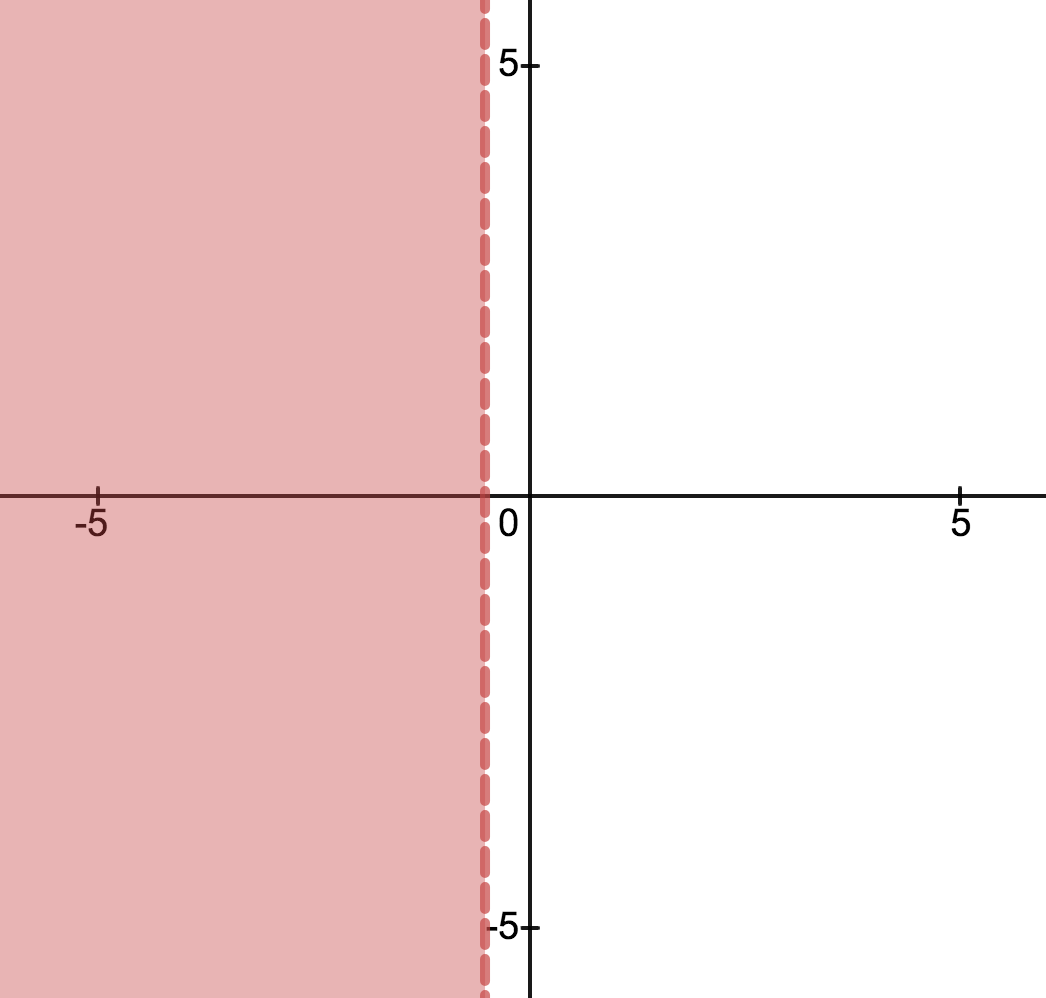
\includegraphics[width = 0.5\textwidth]{4.png}
            \caption{$S$. Plotted in \cite{Desmos}.}
            \label{fig:fig4}
        \end{figure}
        \item Let $z = x + iy \in T$. Then
        \begin{align*}
            8 & \geq |z+1| + |z-3| \\
            |(x+iy) + 1| & \leq 8 - |(x+iy) - 3| \\
            |(x+1) + iy|^2 & \leq \paren{ 8 - |(x-3) + iy| }^2 \\
            (x+1)^2 + y^2 & \leq 64 - 16 |(x-3) + iy| + (x-3)^2 + y^2 \\
            x^2 + 2x + 1 & \leq 64 - 16 |(x-3) + iy| + x^2 - 6x + 9 \\
            8x - 72 & \leq -16 |(x-3) + iy| \\
            8(x-9) & \leq -16 |(x-3) + iy|.
        \end{align*}
        Since $|(x-3) + iy| \geq 0$, we rewrite the last inequality as 
        \[
            9 - x \geq 2 |(x-3) + iy|.
        \]
        Squaring both sides gives
        \begin{align*}
            (9-x)^2 & \geq 4 \paren{ (x-3)^2 + y^2 } \\
            81 - 18x + x^2 & \geq 4(x^2 - 6x + 9 + y^2) \\
            & \geq 4x^2 - 24x + 36 + 4y^2 \\
            3x^2 - 6x + 4y^2 & \leq 45 \\
            3(x^2 - 2x)  + 4y^2 & \leq 45 \\
            3(x^2 - 2x + 1) - 3 + 4y^2 & \leq 45 \\
            3(x-1)^2 + 4y^2 & \leq 48 \\
            \frac{1}{16}(x-1)^2 + \frac{1}{12}y^2 & \leq 1,
        \end{align*}
        so $T$ is the interior of an ellipse (including the boundary) centered at $(1,0)$ with major axis $4$ and minor axis $2\sqrt{3}$. Therefore $T$ is closed.
        \begin{figure}[H]
            \centering
            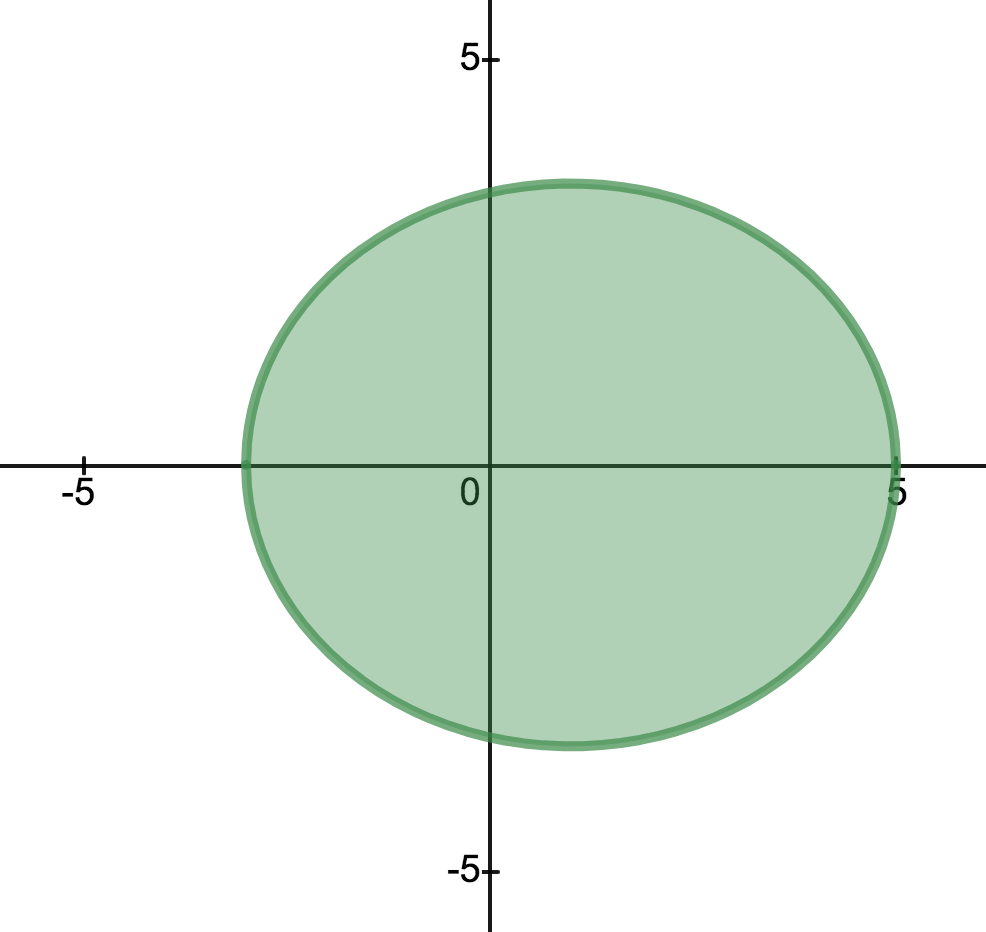
\includegraphics[width = 0.5\textwidth]{5.png}
            \caption{$T$. Plotted in \cite{Desmos}.}
            \label{fig:fig5}
        \end{figure}
    \end{enumerate}
\end{proof}
\subsection{Problem 6 \texorpdfstring{\cite{Conway,Elbow}}{}}
Prove that the set of all linear fractional transformations form a group under composition.
\begin{proof}[Answer]
    Recall that a linear fractional transformation is a map $f : \cx_{\infty} \to \cx_{\infty}$ given by 
    \[
        f(z) = \frac{az + b}{cz + d}
    \]
    for some $a,b,c,d \in \cx$ such that $ad - bc \neq 0$. Let $\mathcal{F}$ denote the set of all such maps. We show that $\mathcal{F}$ is a group under function composition.
    \begin{enumerate}[(i)]
        \item Closure: Let $f_i \in \mathcal{F}$, where 
        \[
            f_i(z) = \frac{a_iz + b_i}{c_iz + d_i}
        \]
        for some $a_i,b_i,c_i,d_i \in \cx$ such that $a_id_i - b_i c_i \neq 0$, for $i = 1 , 2$. Then 
        \begin{align*}
            (f_1 \circ f_2)(z) & = f_1 \paren{ \frac{a_2z + b_2}{c_2z + d_2} } = \frac{a_1 \paren{ \frac{a_2z + b_2}{c_2z + d_2} } + b_1}{c_1 \paren{ \frac{a_2z + b_2}{c_2z + d_2} } + d_1} \\[0.2 em]
            & = \frac{a_1 a_2 z + a_1 b_2 + b_1 c_2 z + b_1 d_2}{ c_2 z + d_2 } \cdot \frac{ c_2 z + d_2 }{ c_1 a_2 z + c_1 b_2 + d_1 c_2 z + d_1 d_2 } \\[0.2 em]
            & = \frac{ \paren{ a_1 a_2 + b_1 c_2 } z + a_1 b_2 + b_1 d_2 }{ \paren{ c_1 a_2 + d_1 c_2 } z + c_1 b_2 + d_1 d_2 }.
        \end{align*}
        Furthermore,
        \begin{align*}
            & \paren{ a_1 a_2 + b_1 c_2 } \paren{ c_1 b_2 + d_1 d_2 } - \paren{ a_1 b_2 + b_1 d_2 } \paren{ c_1 a_2 + d_1 c_2 } \\
            & = a_1 a_2 c_1 b_2 + a_1 a_2 d_1 d_2 + b_1 c_2 c_1 b_2 + b_1 c_2 d_1 d_2 \\
            & - a_1 b_2 c_1 a_2 - a_1 b_2 d_1 c_2 - b_1 d_2 c_1 a_2 - a_1 b_2 d_1 c_2 \\
            & = a_1 d_1 \paren{ a_2 d_2 - b_2 c_2 } - b_1 c_1 \paren{ a_2 d_2 - b_2 c_2 } \\
            & = \paren{ a_1 d_1 - b_1 c_1 } \paren{ a_2 d_2 - b_2 c_2 } \\
            & \neq 0
        \end{align*}
        since $a_i d_i - b_i c_i \neq 0$ for $i = 1 , 2$. Therefore $\mathcal{F}$ is closed under function composition.
        \item Associative: As composition of functions is associative, $(\mathcal{F},\circ)$ is associative.
        \item Identity: The identity map $z \mapsto z$ is a linear fractional transformation, with $a = d = 1$ and $b = c = 0$.
        \item Inverse: Let $f \in \mathcal{F}$, and write 
        \[
            f(z) = \frac{az + b}{cz + d}
        \]
        where $ad - bc \neq 0$. We claim that 
        \[
            g(z) = \frac{dz - b}{-cz + a}
        \]
        is the inverse of $f$ in $\mathcal{F}$. Firstly, 
        \[
            da - (-b)(-c) = ad - bc \neq 0,
        \]
        and so $g \in \mathcal{F}$. Next, 
        \begin{align*}
            (f \circ g)(z) & = \frac{ a \paren{ \frac{dz - b}{-cz + a} } + b }{ c \paren{ \frac{dz - b}{-cz + a} } + d } = \frac{ \frac{adz - ab - bcz + ab }{ -cz + a } }{ \frac{ cdz - bc - dcz + ad }{ -cz + a } } = \frac{(ad - bc)z}{(ad - bc)}.
        \end{align*}
        Since $ad - bc \neq 0$, $(f \circ g)(z) = z$. Furthermore, 
        \begin{align*}
            (g \circ f)(z) & = \frac{ d \paren{ \frac{az + b}{cz + d} } - b }{-c \paren{ \frac{az + b}{cz + d} } + a } = \frac{adz + bd - bc - bd}{cz + d} \cdot \frac{cz + d}{-acz - bc + acz + ad} \\
            & = \frac{(ad - bc)z}{ad - bc} = z.
        \end{align*}
        Therefore $(f \circ g)(z) = (g \circ f)(z) = z$ for all $z \in \cx_{\infty}$, and so $g$ is the inverse of $f$ in $(\mathcal{F},\circ)$.
    \end{enumerate}
    Therefore $(\mathcal{F},\circ)$ is a group.
\end{proof}
Note that there is another (and much more elegant) way to talk about the linear fractional transformations of $\cx_{\infty}$ as the projective linear group $\mathrm{PGL}$ of $\p^1(\cx) \cong \cx_{\infty}$. Then the group structure is automatic!
\newpage
\section{Fall 1992 [Completed]}
A complete paper consists of answering 5 parts from each section. If you work on more than 5 parts on a section, make it clear which 5 parts you wish considered. Show all work you want considered and cross out or erase any extraneous work you do not wish considered.
\subsection{Problem 1}
Let $\displaystyle f(z) = \frac{e^{\frac{1}{z}}}{z}$.
\begin{enumerate}[a)]
    \item Write the Laurent Expansion for $f$ about $0$.
    \item Compute the residue of $f$ at $0$.
    \item Evaluate $\displaystyle \int_C f(z) \, \mathrm{d}z$, where $C$ is the curve $z = e^{i \theta}$, $0 \leq \theta \leq 2\pi$.
\end{enumerate}
\begin{proof}[Answer]
    \noindent
    \begin{enumerate}[a)]
        \item Using 
        \[
            e^z = \sum\limits_{n = 0}^{\infty} \frac{z^n}{n!},
        \]
        we have 
        \[
            \frac{e^{\frac{1}{z}}}{z} = \frac{1}{z} \sum\limits_{n = 0}^{\infty} \frac{z^{-n}}{n!} = \sum\limits_{n = 1}^{\infty} \frac{z^{-n}}{n!}.
        \]
        \item The residue is given by $a_{-1}$, so 
        \[
            \Res(f;0) = \boxed{ 1. }
        \]
        \item Note $f$ is analytic everywhere except at the isolated (and in fact essential) singularity $z = 0$. Since $C$ is a closed rectifiable curve in $\cx \setminus \setb{ 0 }$, 
        \[
            \int_C f(z) \, \mathrm{d}z = 2\pi i n(C;0) \Res(f;0),
        \]
        where $n(C;0)$ is the winding number of $C$ around $z = 0$. Then
        \[
            \int_C f(z) \, \mathrm{d}z = 2\pi i \times 1 \times 1 = \boxed{ 2\pi i. }
        \]
    \end{enumerate}
\end{proof}
\subsection{Problem 2}
Let $f(z) = \Log z$, the principal branch of the logarithm. 
\begin{enumerate}[a)]
    \item Compute $\Log i$.
    \item Indicate the domain $D$ on which $f$ is defined.
    \item Prove $\displaystyle f'(z) = \frac{1}{z}$ for all $z \in D$.
    \item Sketch a well-labeled diagram of the set $f(D) = \setb{ w : w = f(z) \text{ for some } z \in D }$. 
\end{enumerate}
\begin{proof}[Answer]
    \noindent
    \begin{enumerate}[a)]
        \item Writing $z = re^{i \theta}$ for $r > 0$, $-\pi < \theta < \pi$,
        \[
            \Log(z) = \log(r) + i \theta.
        \]
        Then $i = 1 e^{i \frac{\pi}{4}}$, so 
        \[
            \Log i = \log(1) + i \frac{\pi}{4} = \boxed{ \frac{\pi i}{4} . }
        \]
        \item $\Log$ is only defined for $r > 0$ and $-\pi < \theta < \pi$, so 
        \[
            D = \cx \setminus \setb{ x \in \real \mid x \leq 0 }.
        \]
        \item Note that $e^{\Log(z)} = z$ for all $z \in D$. Since $\Log$ is analytic on $D$, we can use Chain Rule to obtain 
        \begin{align*}
            1 & = e^{\Log(z)}\Log'(z) = z \Log'(z) \\
            \Log'(z) & = \frac{1}{z}.
        \end{align*}
        \item Use
        \[
            \Log(z) = \log(r) + i \theta.
        \]
        for $r > 0$, $-\pi < \theta < \pi$. Since $r > 0$ is arbitrary, $\log(r)$ can be any real number. Thus 
        \[
            f(D) = \real \times (-\pi , \pi).
        \]
        \begin{figure}[H]
            \centering
            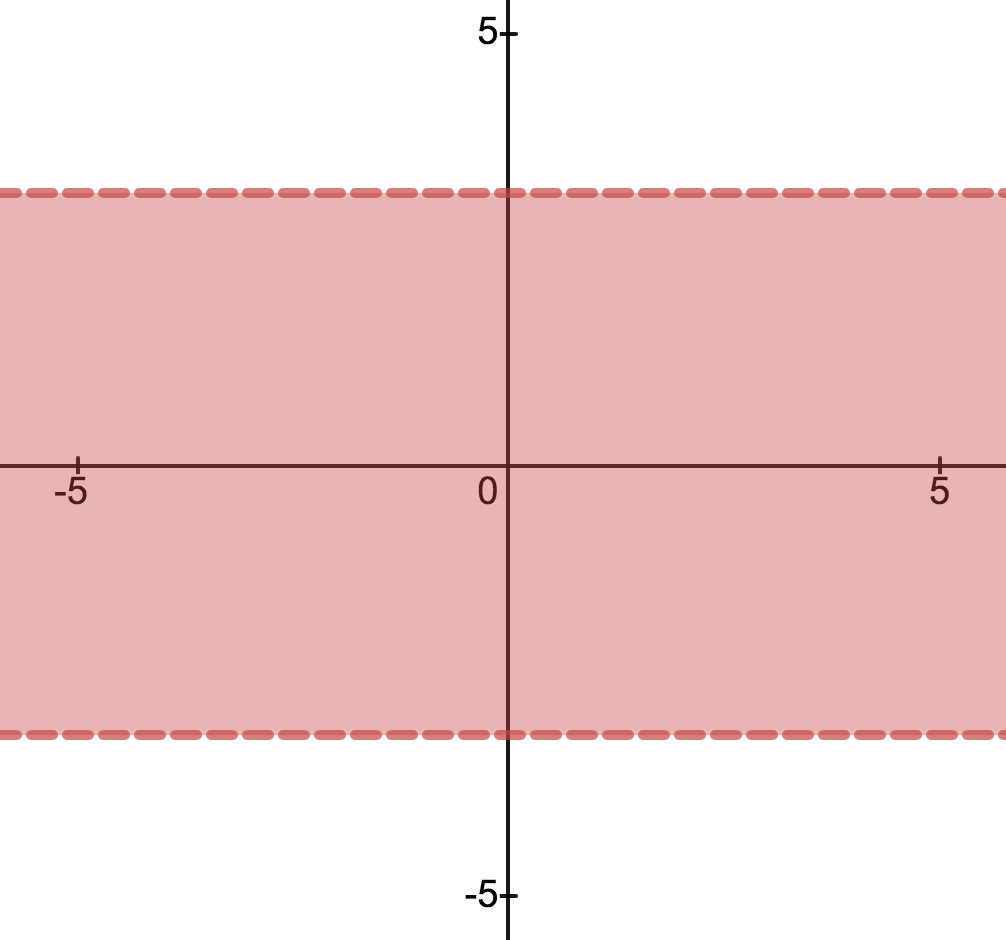
\includegraphics[width = 0.5\textwidth]{2.png}
            \caption{Plotted in \cite{Desmos}.}
            \label{fig:fig3}
        \end{figure}
    \end{enumerate}
\end{proof}
\subsection{Problem 3}
Prove: If $f$ is analytic within and on the simple closed contour $C$, then 
\[
    \int_C \frac{f(z)}{z-z_0}\, \mathrm{d} z = \int_C \frac{f'(z)}{(z-z_0)^2} \, \mathrm{d} z
\]
for every complex $z_0$ not on $C$.
\begin{proof}[Answer]
    There is a typo in this question! It should say
    \[
        \int_C \frac{f'(z)}{z-z_0}\, \mathrm{d} z = \int_C \frac{f(z)}{(z-z_0)^2} \, \mathrm{d} z.
    \]
    For a quick counterexample to the original question, take $f(z) \coloneqq z+1$, $C \coloneqq \setb{ e^{it} \, \middle| \, 0 \leq t \leq 2\pi }$, $z_0 \coloneqq 0$.
    
    Now, let's solve the correct question! By Jordan Curve Theorem, $C$ separates the plane into two regions, \ita{i.e.}, $\cx \setminus C = U \uplus V$, where $U,V \subsetneq \cx$ are open and connected, $U$ is bounded, and $V$ is unbounded. 
    
    Then $f$ is analytic on $U \uplus C$, and for all $z \in \cx \setminus \paren{ U \uplus C } = V$, $n(C;z) = 0$. By Cauchy's Formula, 
    \begin{align*}
        \int_C \frac{f(z)}{\paren{z-z_0}^2}\, \mathrm{d} z & = \int_C \frac{f(z)}{\paren{z-z_0}^{1+1}}\, \mathrm{d} z = \frac{2\pi i}{1!} n(C;z_0) f^{(1)}(z_0) = 2\pi i n(C;z_0) f'(z_0)
    \end{align*}
    for all $z_0 \in U$. Since $f$ is analytic on $U \uplus C$, so is $f'$, and applying Cauchy's Formula to $f'$ gives us 
    \[
        \int_C \frac{f'(z)}{z-z_0} \, \mathrm{d} z = 2\pi i n(C;z_0) f'(z_0)
    \]
    for all $z_0 \in U$. Hence the two integrals are equal for $z_0 \in U$. For $z_0 \in V$, then both integrands are analytic on $U \uplus C$, and so both integrals are equal to zero by Cauchy's Theorem. 
\end{proof}
\subsection{Problem 4}
\begin{enumerate}[a)]
    \item Write the Taylor expansion for $\displaystyle f(z) = \frac{1}{1 - z}$ valid in the unit disk $|z| < 1$.
    \item Use that Taylor expansion together with allowable operations to obtain an expansion for $\displaystyle g(z) = \frac{z}{(1-z)^2}$ valid in $|z| < 1$.
    \item Use the expansion for $g$ to calculate the sum 
    \[
        \frac{1}{2} + \frac{2}{4} + \frac{3}{8} + \dotsb + \frac{n}{2^n} + \dotsb = \sum\limits_{n = 1}^{\infty} n 2^{-n}.
    \]
\end{enumerate}
\begin{proof}[Answer]
    \noindent
    \begin{enumerate}[a)]
        \item Using the geometric series, we have 
        \[
            f(z) = \sum\limits_{n = 0}^{\infty} z^n
        \]
        for $|z| < 1$.
        \item Since $f$ is analytic in the unit disk, it has a derivative
        \begin{align*}
            f'(z) & = \frac{-1}{-(1-z)^{-2}} = \frac{1}{(1-z)^2} = \frac{g(z)}{z}.
        \end{align*}
        Differentiating the Taylor series for $f$ term by term gives us
        \begin{align*}
            \frac{g(z)}{z} & = f'(z) = \sum\limits_{n = 0}^{\infty} n z^{n-1} = \sum\limits_{n = 1}^{\infty} n z^{n-1}.
        \end{align*}
        Hence
        \[
            g(z) = z \sum\limits_{n = 1}^{\infty} n z^{n-1} = \sum\limits_{n = 1}^{\infty} n z^n.
        \]
        \item 
        \begin{align*}
            \sum\limits_{n = 1}^{\infty} n 2^{-n} & = \sum\limits_{n = 1}^{\infty} n \paren{ \frac{1}{2} }^n = g \paren{ \frac{1}{2} } \\
            & = \frac{ \frac{1}{2} }{ \paren{ 1 - \frac{1}{2} }^2 } = \frac{1}{2} \times \frac{1}{ \frac{1}{4} } \\
            & = \boxed{ 2. }
        \end{align*}
    \end{enumerate}
\end{proof}
\subsection{Problem 5}
Evaluate $\displaystyle \int_0^{\infty} \frac{\mathrm{d}x}{(1+x^2)^2}$ using residues.
\begin{proof}[Answer]
    Consider 
    \[
        I \coloneqq \int_0^{\infty} \frac{ \mathrm{d}x }{ \paren{ 1 + x^2 }^2 }.
    \]
    Note that $\frac{1}{ \paren{ 1 + x^2 }^2 }$ is an even function, and so 
    \[
        I = \frac{1}{2} \int_{-\infty}^{\infty} \frac{ \mathrm{d}x }{ \paren{ 1 + x^2 }^2 }.
    \]
    Let 
    \[
        f(z) \coloneqq \frac{1}{ \paren{ 1 + z^2 }^2 } = \frac{1}{(z - i)(z + i)}.
    \]
    $f$ is meromorphic with poles at $z = \pm i$ of order 2. Let $R > 1$, and let $\gamma$ be the same curve as in Spring 1992, Problem 1 (see \ref{fig:fig1}). Then by the Residue Theorem,
    \[
        \int_{\gamma} f(z) \, \mathrm{d}z = 2\pi i \Res(f;i).
    \]
    Then 
    \begin{align*}
        \Res(f;i) & = \frac{ \mathrm{d} }{ \mathrm{d} z} \left. \sqbrack{ \frac{1}{(z+i)^2} } \right|_{ z = i } = \left. -\frac{2}{(z+i)^3} \right|_{z = i} \\
        & = -\frac{2}{(2i)^3} = -\frac{2}{-8i} \\
        & = -\frac{i}{4}.
    \end{align*}
    Thus 
    \[
        \int_{\gamma} f(z) \, \mathrm{d}z = 2\pi i \times -\frac{i}{4} = \frac{\pi}{2}.
    \]
    Write
    \[
        \int_{\gamma} f(z) \, \mathrm{d}z = \int_{-R}^R \frac{ \mathrm{d}x }{ \paren{ 1 + x^2 }^2 } + \underbrace{ \int_0^{\pi} \frac{ iRe^{it} }{ \paren{ 1 + R^2e^{2it} }^2 } \, \mathrm{d}t }_{ \eqqcolon I(R) }.
    \]
    Then 
    \begin{align*}
        0 & \leq |I(R)| \\
        & = \left| iR \int_0^{\pi} \frac{ e^{it} }{ \paren{ 1 + R^2e^{2it} }^2 } \, \mathrm{d}t \right| \\
        & \leq R \int_0^{\pi} \frac{1}{ \left| 1 + R^2e^{2it} \right|^2 } \, \mathrm{d}t \\
        & \leq R \int_0^{\pi} \frac{ \mathrm{d}t }{R^2 - 1} && \text{see Spring 1992, Problem 1 for more explanation} \\
        & = \frac{ \pi R }{ R^2 - 1 } \\
        & \to 0
    \end{align*}
    as $R \to \infty$. Thus 
    \begin{align*}
        2I & = \int_{-\infty}^{\infty} \frac{ \mathrm{d}x }{ \paren{ 1 + x^2 }^2 } = \lim\limits_{R \to \infty} \sqbrack{ \int_{-R}^R \frac{ \mathrm{d}x }{ \paren{ 1 + x^2 }^2 } } \\
        & = \lim\limits_{R \to \infty} \sqbrack{ \frac{\pi}{2} - I(R) } = \frac{\pi}{2} - 0 \\
        & = \frac{\pi}{2}.
    \end{align*}
    Therefore 
    \[
        I = \boxed{ \frac{\pi}{4}. }
    \]
    Again, this integral can be evaluated using real variable methods.
\end{proof}

\subsection{Problem 6 \texorpdfstring{\cite{Conway}}{}}
State Rouch\'e's Theorem and use it to prove that every nonconstant polynomial has a complex root.
\begin{proof}[Answer]
    Suppose that $f$ and $g$ are meromorphic in a neighborhood of $\bar{B}(a;R)$ with no zeros or poles on the circle $\gamma = \partial B(a;R)$. If $Z_f,Z_g$ ($P_f,P_g$) are the number of zeros (poles) of $f$ and $g$ in $B(a;R)$ counted with multiplicity and if 
    \[
        |f(z) + g(z)| < |g(z)|
    \]
    on $\gamma$, then 
    \[
        Z_f - P_f = Z_g - P_g.
    \]
    Now, let $p \in \cx[z]$ be a nonconstant polynomial of degree $n \in \z^+$. Without loss of generality, take $p$ to be a monic polynomial, so we can write 
    \[
        p(z) = a_0 + a_1 z + \dotsb + a_{n-1} z^{n-1} + z^n.
    \]
    Then 
    \[
        \frac{p(z)}{z^n} = \frac{a_0}{z^n} + \frac{a_1}{z^{n-1}} + \dotsb + \frac{a_{n-1}}{z} + 1,
    \]
    and so 
    \begin{align*}
        \abs{ \frac{p(z)}{z^n} } & = \abs{ \frac{a_0}{z^n} + \frac{a_1}{z^{n-1}} + \dotsb + \frac{a_{n-1}}{z} + 1 } \\
        & \leq \abs{ \frac{a_0}{z^n} } + \abs{ \frac{a_1}{z^{n-1}} } + \dotsb + \abs{ \frac{a_{n-1}}{z} } + \abs{ 1 } \\
        & \to 0 + 0 + \dotsb + 0 + 1 \\
        & = 1
    \end{align*}
    as $z \to \infty$. Thus there exists $R > 0$ large enough such that 
    \[
        \abs{ \frac{p(z)}{z^n} - 1 } < 1
    \]
    for $|z| = R$. Then 
    \[
        \abs{z} > \abs{z}\abs{ \frac{p(z)}{z^n} - 1 } = \abs{ p(z) - z^n }
    \]
    for all $|z| = R$. By Rouch\'e's Theorem, 
    \[
        Z_p - P_p = Z_{z^n} - P_{z^n}.
    \]
    Since $p(z)$ and $z^n$ are entire, $P_p = P_{z^n} = 0$. Thus $Z_p = n$.
\end{proof}

\subsection{Problem 7}
Obtain a harmonic conjugate for $u(x,y) = y^3 - 3x^2 y$.
\begin{proof}[Answer]
    A harmonic conjugate for $u$ is a function $v \in C^1(\real^2,\real)$ satisfying
    \[
        u_x(x,y) = v_y(x,y) , \qquad u_y(x,y) = -v_x(x,y)
    \]
    for all $(x,y) \in \real^2$. Then 
    \begin{align*}
        v_y(x,y) & = -6xy \\
        v_x(x,y) & = 3x^2 - 3y^2,
    \end{align*}
    so 
    \begin{align*}
        v(x,y) = -3xy^2 + h_1(x) = x^3 - 3xy^2 + h_2(y)
    \end{align*}
    for some $h_1 , h_2 \in C^1(\real,\real)$. Thus $h_1(x) = x^3$ and $h_2(y) = 0$, and so 
    \[
        v(x,y) = x^3 - 3xy^2
    \]
    is a harmonic conjugate to $u$.
\end{proof}
\subsection{Problem 8}
Find \underline{all} entire functions $f$ that satisfy $|f(z)| \leq |e^z|$ for all complex $z$. (Hint: Use Liouville's theorem appropriately.)
\begin{proof}[Answer]
    By inspection, $f_w : \cx \to \cx$ given by $f_w(z) = w e^z$ for a fixed $w \in \cx$ with $|w| \leq 1$ is an entire function that satisfies $|f_w(z)| \leq |e^z|$ for all $z \in \cx$. We claim all entire functions that satisfy $|f(z)| \leq |e^z|$ for all $z \in \cx$ must be of this form. Let $f : \cx \to \cx$ be an entire function satisfying the inequality, then $g(z) \coloneqq f(z)e^{-z}$ is also entire (since $e^{z} \neq 0$ for all $z \in \cx$) and satisfies
    \[
        |g(z)| = \left| \frac{f(z)}{e^z} \right| \leq 1
    \]
    for all $z \in \cx$. By Liouville's Theorem, $g$ is constant and so $g(z) \equiv w$ for some $\alpha \in \cx$. Then $|w| \geq 1$ and so 
    \[
        f(z) = w e^z.
    \] 
\end{proof}
\newpage
\section{Winter 1993 [Answered]}
Answer five questions from each part. Please be sure it is clear which questions you want graded. All problems count 10 points. This exam will test the extent of your knowledge and the clarity of your mathematical writing. Please do not write mush.
\subsection{Problem 1}
Find the Laurent expansion of $\displaystyle \frac{1}{\paren{1+z^2}\paren{2+z^2}}$ in each of the following regions.
\begin{enumerate}[(i)]
    \item $1 < |z| < \sqrt{2}$ (an annulus)
    \item $\sqrt{2} < |z|$ (the exterior of a disk)
\end{enumerate}
\begin{proof}[Answer]
    Let 
    \[
        f(z) \coloneqq \frac{1}{\paren{1+z^2}\paren{2+z^2}} = \frac{1}{z^2 + 1} + \frac{1}{z^2 + 2}.
    \]
    First, expand $f$ in partial fraction decomposition. We tackle each quadratic term separately. Write
    \[
        \frac{1}{z^2 + 1} = \frac{A}{z - i} + \frac{B}{z + i}
    \]
    for some undetermined $A , B \in \cx$. Then 
    \[
        1 = A(z + i) + B(z - i) = (A + B)z + (A - B)i.
    \]
    Then $A + B = 0$ and $A - B = -i$. Thus $B = -A$, and so $2A = -i$, or $A = -\frac{i}{2}$. This gives $B = \frac{i}{2}$, and so 
    \[
        \frac{1}{z^2 + 1} = \frac{i}{2} \paren{ \frac{1}{z + i} - \frac{1}{z - i} }.
    \]
    Similarly, 
    \[
        \frac{1}{z^2 + 2} = \frac{i\sqrt{2}}{2} \paren{ \frac{1}{z + \sqrt{2} i} - \frac{1}{z - \sqrt{2} i} }.
    \]
    Thus 
    \[
        f(z) = \frac{i}{2} \paren{ \frac{1}{z + i} - \frac{1}{z - i} + \frac{\sqrt{2}}{z + \sqrt{2} i} - \frac{\sqrt{2}}{z - \sqrt{2} i} }.
    \]
    \begin{enumerate}[(i)]
        \item We expand each summand about $z = 0$:
        \begin{align*}
            \frac{1}{z + i} & = \frac{1}{z \paren{ 1 + \frac{i}{z} } } = \frac{1}{z} \sum\limits_{n = 0}^{\infty} \paren{ -\frac{i}{z} }^n = \sum\limits_{n = 1}^{\infty} (-i)^{n-1} z^{-n},
        \end{align*}
        for $\left| -\frac{i}{z} \right| < 1$, or equivalently $|z| > 1$. Similarly,
        \[
            \frac{1}{z - i} = \sum\limits_{n = 1}^{\infty} i^{n-1} z^{-n}
        \]
        for $|z| > 1$. Next,
        \begin{align*}
            \frac{1}{z + \sqrt{2}i} & = \frac{1}{\sqrt{2}i \paren{ 1 + \frac{z}{\sqrt{2}i} } } = -\frac{i}{\sqrt{2}} \sum\limits_{n = 0}^{\infty} \paren{ - \frac{z}{\sqrt{2}i} }^n =  -\frac{i}{\sqrt{2}} \sum\limits_{n = 0}^{\infty} \paren{ \frac{i}{\sqrt{2}} }^n z^n,
        \end{align*}
        for $\left| - \frac{z}{\sqrt{2}i} \right| < 1$, or equivalently $|z| < \sqrt{2}$. Similarly,
        \[
            \frac{1}{z - \sqrt{2}i} = \frac{i}{\sqrt{2}} \sum\limits_{n = 0}^{\infty} \paren{ -\frac{i}{\sqrt{2}} }^n z^n.
        \]
        Substituting these sums into $f$ is valid on intersection of the domains of the sums, which is on $1 < |z| < \sqrt{2}$. Thus for $1 < |z| < \sqrt{2}$,
        \begin{align*}
            f(z) & = \frac{i}{2} \paren{ \frac{1}{z + i} - \frac{1}{z - i} + \frac{\sqrt{2}}{z + \sqrt{2} i} - \frac{\sqrt{2}}{z - \sqrt{2} i} } \\
            & = \frac{i}{2}\sum\limits_{n = 1}^{\infty} (-i)^{n-1} z^{-n} - \frac{i}{2}\sum\limits_{n = 1}^{\infty} i^{n-1} z^{-n}  \\
            & + \frac{i\sqrt{2}}{2} \times -\frac{i}{\sqrt{2}} \sum\limits_{n = 0}^{\infty} \paren{ \frac{i}{\sqrt{2}} }^n z^n - \frac{i\sqrt{2}}{2} \times \frac{i}{\sqrt{2}} \sum\limits_{n = 0}^{\infty} \paren{ -\frac{i}{\sqrt{2}} }^n z^n \\
            & = \frac{1}{2}\sum\limits_{n = 1}^{\infty} -(-i)^{n} z^{-n} - \frac{1}{2}\sum\limits_{n = 1}^{\infty} i^{n} z^{-n} + \frac{1}{2} \sum\limits_{n = 0}^{\infty} \paren{ \frac{i}{\sqrt{2}} }^n z^n + \frac{1}{2} \sum\limits_{n = 0}^{\infty} \paren{ -\frac{i}{\sqrt{2}} }^n z^n \\
            & = \boxed{ \frac{1}{2} \sqbrack{ \sum\limits_{n = 1}^{\infty} \paren{ -i^n - (-i)^n } z^{-n} + \sum\limits_{n = 0}^{\infty} \paren{ \frac{ i^n + (-i)^n }{2^{n/2}} } z^n } . }
        \end{align*}
        \item For $|z| > \sqrt{2}$, we only need to find expansions for $\inv{ \paren{ z \pm \sqrt{2} i } }$. 
        \begin{align*}
            \frac{1}{ z + \sqrt{2}i } & = \frac{1}{z \paren{ 1 + \frac{\sqrt{2}i}{z} } } = \frac{1}{z} \sum\limits_{n = 0}^{\infty} \paren{ -\frac{\sqrt{2}i}{z} }^n= \sum\limits_{n = 1}^{\infty} 2^{ \frac{1}{2}(n-1) } (-i)^{n-1} z^{-n}
        \end{align*}
        for $\left| -\frac{\sqrt{2}i}{z} \right| < 1$, or equivalently $|z| > \sqrt{2}$. Similarly,
        \[
            \frac{1}{ z - \sqrt{2}i } = \sum\limits_{n = 1}^{\infty} 2^{ \frac{1}{2}(n-1) } i^{n-1} z^{-n}
        \]
        for $|z| > \sqrt{2}$. Thus for $|z| > \sqrt{2}$,
        \begin{align*}
            f(z) & = \frac{i}{2} \paren{ \frac{1}{z + i} - \frac{1}{z - i} + \frac{\sqrt{2}}{z + \sqrt{2} i} - \frac{\sqrt{2}}{z - \sqrt{2} i} } \\
            & = \frac{1}{2} \sum\limits_{n = 1}^{\infty} \paren{ -i^n - (-i)^n } z^{-n} + \frac{\sqrt{2}i}{2} \sum\limits_{n = 1}^{\infty} 2^{ \frac{1}{2}(n-1) } (-i)^{n-1} z^{-n} - \frac{\sqrt{2}i}{2} \sum\limits_{n = 1}^{\infty} 2^{ \frac{1}{2}(n-1) } i^{n-1} z^{-n} \\
            & = \frac{1}{2} \sum\limits_{n = 1}^{\infty} \paren{ -i^n - (-i)^n } z^{-n} + \sum\limits_{n = 1}^{\infty} 2^{\frac{1}{2}(n-2)} \paren{ -i^n - (-i)^n } z^{-n} \\
            & = \boxed{ \sum\limits_{n = 1}^{\infty} \paren{ \frac{ 1 + 2^{n/2} }{2} } \paren{ -i^n - (-i)^n } z^{-n}. }
        \end{align*}
    \end{enumerate}
\end{proof}
\subsection{Problem 2 \texorpdfstring{\cite{Conway}}{}}
Suppose that the complex number $a$ satisfies $\displaystyle 0 < |a| < \paren{ \frac{1}{2} }^5$. Show that the equation $(z - 1)^5 e^z = a$ has exactly 5 roots (all distinct) in the disk $\setb{ z \, \middle| \, |z - 1| < \frac{1}{2} }$.
\begin{proof}[Answer]
    We refer to the following theorem:
    \begin{theorem}
        Let $f$ be analytic on $B(a;R)$, $\alpha \coloneqq f(a)$. If $f(z) - \alpha$ has a zero of order $m$ at $z = a$, then there exists $\eps , \delta > 0$ such that for all $0 < |\zeta - a| < \delta$, $f(z) = \zeta$ has exactly $m$ simple roots on $B(a;\eps)$.
    \end{theorem}
    \begin{proof}
        Since the zeros of an analytic function are isolated, there exists $0 < \eps < \frac{1}{2}R$ such that for all $0 < |z-a| < 2\eps$, $f(z) = \alpha$ has no solutions and $f'(z) \neq 0$. Let $\gamma(t) \coloneqq a + \eps e^{it}$, $0 \leq t \leq 2\pi$, and let $\sigma \coloneqq f \circ \gamma$ (note that $\sigma$ is a smooth closed curve). Then $\alpha \notin \sigma \paren{ [0,2\pi] }$, so there exists $\delta > 0$ such that $B(\alpha;\delta) \cap \sigma \paren{ [0,2\pi] } = \varnothing$. So $B(\alpha;\delta)$ must be contained in some component of $\cx \setminus \sigma \paren{ [0,2\pi] }$, thus for all $0 < |\zeta - \alpha| < \delta$,
        \[
            n(\sigma;\alpha) = n(\sigma;\zeta) = \sum\limits_{k = 1}^p n \paren{ \gamma ; z_k },
        \]
        where $z_k$ satisfies $f \paren{ z_k } = \alpha$. But since $n(\gamma;z)$ must either be zero or one, there must be exactly $m$ solutions to the equation $f(z) = \gamma$ inside $B(a;\eps)$. Since $f'(z) \neq 0$ for all $0 < |z-a| < \eps$, each of these roots (for $\zeta \neq \alpha$) must be simple.
    \end{proof}
    For simplicity we rename all variables to be consistent with the statement of the theorem. Then $f(z) \coloneqq (z-1)^5 e^{z}$, $a \coloneqq 1$, and $\alpha = f(1) = 0$. Thus $f(z) - \alpha = f(z)$ has a zero of order 5 at $z = 1$. Then since $\zeta$ satisfies 
    \[
        0 < |\zeta| = |\zeta - \alpha| < \frac{1}{32},
    \]
    it suffices to show that $\eps = \frac{1}{2}$ is enough to show that $f(z) = \zeta$ has 5 simple roots on $|z-1| < \eps$. 
    
    Let $\gamma(t) \coloneqq 1 + \frac{1}{2}e^{it}$, $0 \leq t \leq 2\pi$. Then 
    \begin{align*}
        \sigma(t) & = f \paren{ \gamma(t) } = \paren{ 1 + \frac{1}{2}e^{it} - 1 }^5 e^{1 + \eps e^{it}} \\
        & = \frac{1}{2^5} e^{5it} e^{1 + \eps e^{it}} = \frac{1}{32} e^{ 1 + \frac{11}{2} e^{it}}.
    \end{align*}
    Then $\sigma(t) \neq 0 = \alpha$ for all $0 \leq t \leq 2\pi$, and in fact
    \begin{align*}
        \abs{ \sigma(t) } & = \abs{ \sigma(t) - 0 } = \abs{ \frac{1}{32} e^{ 1 + \frac{11}{2} e^{it}} } = \frac{1}{32},
    \end{align*}
    and so for all $0 < |\zeta - 0| < \frac{1}{32}$, $f(z) = \zeta$ has exactly 5 distinct solutions on $|z-1| < \frac{1}{2}$.
\end{proof}
\subsection{Problem 3 \texorpdfstring{\cite{Conway}}{}}
Let $G$ be a bounded open connected set in the complex plane. Suppose that $f$ is an analytic function on an open connected set $H$ that contains the closure of $G$. Suppose that $f$ is \underline{nonconstant} on $G$ and $|f|$ is constant on the boundary of $G$. Show that $f$ must have a zero in $G$.
\begin{proof}[Answer]
    Since $G$ is bounded, open, and connected and $f$ is analytic on $\overline{G}$, by Maximum Modulus Theorem we have
    \[
        \max \setb{ \abs{f(z)} \, \middle| \, z \in \overline{G} } = \max \setb{ \abs{f(z)} \, \middle| \, z \in \partial G }.
    \]
    Now, if $|f| = 0$ on $\partial G$ then $f = 0$ on $\overline{G}$, which contradicts $f$ being nonconstant on $G$. Thus assume that $|f(z)| = M > 0$ for all $z \in \partial G$, then $|f(z)| < M$ for all $z \in G$. By way of contradiction, suppose that $0 \notin f(G)$, then $\frac{1}{f(z)}$ is defined and analytic for all $z \in \overline{G}$. By Maximum Modulus Theorem,
    \[
        \max \setb{ \abs{\frac{1}{f(z)}} \, \middle| \, z \in \overline{G} } = \max \setb{ \abs{\frac{1}{f(z)}} \, \middle| \, z \in \partial G }.
    \]
    Since $|f|$ is constant on $\partial G$, so is $\frac{1}{|f|}$ and so 
    \[
        \max \setb{ \abs{\frac{1}{f(z)}} \, \middle| \, z \in \partial G } = \frac{1}{M}.
    \]
    Thus $\frac{1}{|f(z)|} < \frac{1}{M}$ for all $z \in G$, and so we have $M > M$, a contradiction. Therefore $f$ must have a zero in $G$.
\end{proof}
\subsection{Problem 4}
Verify \underline{one} of the following equations.
\begin{multicols}{2}
    \begin{enumerate}[(i)]
        \item $\displaystyle \int_0^{2\pi} \frac{\cos 3 \theta}{5 - 4\cos \theta} \, \mathrm{d} \theta = \frac{\pi}{12}$
        \item $\displaystyle \int_0^{\infty} \frac{ \mathrm{d}x}{x^4 + x^2 + 1} = \frac{\pi \sqrt{3}}{6}$.
    \end{enumerate}
\end{multicols}
\begin{proof}[Answer]
    \noindent
    \begin{enumerate}[(i)]
        \item Let 
        \[
            I \coloneqq \int_0^{2\pi} \frac{\cos 3 \theta}{5 - 4\cos \theta} \, \mathrm{d} \theta.
        \]
        Note that for $z = e^{i\theta}$, $\overline{z} = e^{-i \theta} = \frac{1}{z}$. Then 
        \begin{align*}
            \cos \theta & = \re(z) = \frac{z + \overline{z}}{2} \\
            & = \frac{1}{2} \paren{ z + \frac{1}{z} } = \frac{z^2 + 1}{2z}.
        \end{align*}
        Thus 
        \begin{align*}
            5 - 4 \cos \theta & = 5 - \frac{4(z^2+1)}{2z} = 5 - \frac{2(z^2+1)}{z} \\
            & = \frac{5z - 2z^2 - 2}{z} = \frac{2z^2 - 5z + 2}{-z} \\
            & = \frac{(2z-1)(z-2)}{-z} = -\frac{2\paren{ z - \frac{1}{2} }(z-2)}{z}.
        \end{align*}
        Now, using the sine and cosine addition formulae
        \begin{align*}
            \sin(\theta + \phi) & = \sin \theta \cos \phi + \cos \theta \sin \phi \\
            \cos(\theta + \phi) & = \cos \theta \cos \phi - \sin \theta \sin \phi,
        \end{align*}
        we can rewrite
        \begin{align*}
            \cos(3\theta) & = \cos(2\theta + \theta) \\
            & = \cos(2\theta) \cos \theta - \sin(2\theta) \sin \theta \\
            & = \paren{ \cos \theta \cos \theta - \sin \theta \sin \theta } \cos \theta - \paren{ \sin \theta \cos \theta + \cos \theta \sin \theta } \sin \theta \\
            & = \cos^3 \theta - \cos \theta \sin^2 \theta - \cos \theta \sin^2 \theta - \cos \theta \sin^2 \theta \\
            & = \cos^3 \theta - 3 \cos \theta \sin^2 \theta.
        \end{align*}
        Then using $z = e^{i \theta}$ again, we have
        \begin{align*}
            \sin \theta & = \im(z) = \frac{z - \overline{z}}{2i} \\
            & = \frac{1}{2i} \paren{ z - \frac{1}{z} } = \frac{z^2 - 1}{2iz}.
        \end{align*}
        Now rewrite $\cos(3\theta)$ as 
        \begin{align*}
            \cos(3\theta) & = \cos^3 \theta - 3 \cos \theta \sin^2 \theta = \paren{ \frac{z^2 + 1}{2z} }^3 - 3 \paren{ \frac{z^2 + 1}{2z} } \paren{ \frac{z^2 - 1}{2iz} }^2 \\
            & = \frac{1}{8z^3} \paren{ z^6 + 3z^4 + 3z^2 + 1 } - \frac{3}{2z}(z^2 + 1) \times \frac{1}{-4z^2} \paren{ z^4 - 2z^2 + 1 } \\
            & = \frac{1}{8z^3} \paren{ z^6 + 3z^4 + 3z^2 + 1 } + \frac{3}{8z^3} \paren{ z^6 - 2z^4 + z^2 + z^4 - 2z^2 + 1 } \\
            & = \frac{1}{8z^3} \paren{ z^6 + 3z^4 + 3z^2 + 1 + 3z^6 -3z^4 - 3z^2 + 3 } \\
            & = \frac{1}{8z^3} \paren{ 4z^6 + 4 } = \frac{z^6 + 1}{2z^3}.
        \end{align*}
        Finally,
        \[
            \frac{\cos 3 \theta}{5 - 4\cos \theta} = \frac{z^6 + 1}{2z^3} \times -\frac{z}{2\paren{ z - \frac{1}{2} }(z-2)} = -\frac{ \paren{ z^6 + 1 } z }{ 4 z^3 \paren{ z - \frac{1}{2} }(z-2) }.
        \]
        Let $\gamma$ be the unit circle, \ita{i.e.}, $\gamma : [0,2\pi] \to \cx$, $\gamma(\theta) \coloneqq e^{i \theta}$. Then 
        \begin{align*}
            \int_0^{2\pi} \frac{\cos 3 \theta}{5 - 4\cos \theta} \, \mathrm{d} \theta & = -\int_0^{2\pi} \frac{ \paren{ z^6 + 1 } z }{ 4 z^3 \paren{ z - \frac{1}{2} }(z-2) } \, \mathrm{d} \theta = i \int_0^{2\pi} \frac{ \paren{ z^6 + 1 } i e^{i \theta} }{ 4 z^3 \paren{ z - \frac{1}{2} }(z-2) } \, \mathrm{d} \theta \\
            & = i \int_{\gamma} \frac{ z^6 + 1 }{ 4 z^3 \paren{ z - \frac{1}{2} }(z-2) } \, \mathrm{d}z.
        \end{align*}
        Let 
        \[
            f(z) \coloneqq \frac{ z^6 + 1 }{ 4 z^3 \paren{ z - \frac{1}{2} }(z-2) },
        \]
        then $f$ is meromorphic with a \ita{triple} pole (yikes!) at $z = 0$, a simple pole at $z = \frac{1}{2}$, and a simple pole at $z = 2$. Since $\gamma$ encircles $z = 0$ and $z = \frac{1}{2}$, 
        \[
            \int_0^{2\pi} \frac{\cos 3 \theta}{5 - 4\cos \theta} \, \mathrm{d} \theta = i \int_{\gamma} \frac{ z^6 + 1 }{ 4 z^3 \paren{ z - \frac{1}{2} }(z-2) } \, \mathrm{d}z = i (2\pi i) \sqbrack{ \Res(f;0) + \Res \paren{f ; \frac{1}{2} } }.
        \]
        Let's tackle the easy one first. 
        \begin{align*}
            \Res \paren{f ; \frac{1}{2} } & = \lim\limits_{z \to \frac{1}{2} } \paren{ z - \frac{1}{2} } f(z) = \lim\limits_{z \to \frac{1}{2} } \frac{ \paren{ z - \frac{1}{2} } \paren{ z^6 + 1 } }{ 4 z^3 \paren{ z - \frac{1}{2} }(z-2) } = \left. \frac{ z^6 + 1 }{ 4 z^3 (z-2) } \right|_{ z = \frac{1}{2} } \\
            & = \frac{1}{4} \paren{ \frac{1}{2^6} + 1 } \times 2^3 \times \frac{1}{\frac{1}{2} - 2} = 2 \times \paren{ \frac{1}{64} + 1 } \times -\frac{2}{3} \\
            & = -\frac{4}{3} \times \frac{65}{64} = -\frac{65}{48}.
        \end{align*}
        Now, let's take on the triple pole. 
        \begin{align*}
            \Res(f;0) & = \frac{1}{(3-1)!} \frac{\mathrm{d}^{3-1}}{\mathrm{d}z^{3-1}} \left. \sqbrack{ (z - 0)^3 f(z) } \right|_{z = 0} = \frac{1}{2!} \frac{\mathrm{d}^{2}}{\mathrm{d}z^{2}} \left. \sqbrack{ \frac{ z^3 \paren{ z^6 + 1 } }{ 4 z^3 \paren{ z - \frac{1}{2} }(z-2) } } \right|_{z = 0} \\
            & = \frac{1}{2} \frac{\mathrm{d}^{2}}{\mathrm{d}z^{2}} \left. \sqbrack{ \frac{ z^6 + 1  }{ 4 \paren{ z - \frac{1}{2} }(z-2) } } \right|_{z = 0} = \frac{1}{2} \frac{\mathrm{d}^{2}}{\mathrm{d}z^{2}} \left. \sqbrack{ \frac{ z^6 + 1  }{ 4z^2 - 10z + 4 } } \right|_{z = 0} 
        \end{align*}
        Ok, let's take that derivative.
        \begin{align*}
            \Res(f;0) & = \frac{1}{2} \frac{\mathrm{d}}{\mathrm{d}z} \left. \sqbrack{ \frac{ \paren{ 4z^2 - 10z + 4 } \paren{ 6z^5 } - \paren{ z^6 + 1 } \paren{ 8z - 10 } }{ \paren{ 4z^2 - 10z + 4 }^2 } } \right|_{z = 0} \\ 
            & = \frac{1}{2} \frac{\mathrm{d}}{\mathrm{d}z} \left. \sqbrack{ \frac{ 24z^7 - 60z^6 + 24z^5 - 8z^7 + 10z^6 - 8z + 10 }{ \paren{ 4z^2 - 10z + 4 }^2 } } \right|_{z = 0} \\ 
            & = \frac{1}{2} \frac{\mathrm{d}}{\mathrm{d}z} \left. \sqbrack{ \frac{ 16z^7 - 50z^6 + 24z^5 - 8z + 10 }{ \paren{ 4z^2 - 10z + 4 }^2 } } \right|_{z = 0} \\ 
            & = \frac{\mathrm{d}}{\mathrm{d}z} \left. \sqbrack{ \frac{ 8z^7 - 25z^6 + 12z^5 - 4z + 5 }{ \paren{ 4z^2 - 10z + 4 }^2 } } \right|_{z = 0}.
        \end{align*}
        Breathe slowly. Take that derivative one more time.
        \begin{align*}
            \Res(f;0) & = \left. \frac{ \paren{ 4z^2 - 10z + 4 }^2 \paren{ 56z^6 - 150z^5 + 60z^4 - 4 } }{ \paren{ 4z^2 - 10z + 4 }^4 } \right|_{z = 0} \\
            & - \left. \frac{ \paren{ 8z^7 - 25z^6 + 12z^5 - 4z + 5 } 2\paren{ 4z^2 - 10z + 4 } \paren{ 8z^2 - 10 } }{ \paren{ 4z^2 - 10z + 4 }^4 } \right|_{z = 0} \\[0.2em]
            & = \frac{ \paren{ 4 }^2 \paren{ - 4 } -2\paren{ 5 } \paren{ 4 } \paren{ - 10 } }{ \paren{ 4 }^4 }  = \frac{-64 + 600}{256} \\[0.2em]
            & = \frac{536}{256} = \frac{63}{48}.
        \end{align*}
        Finally,
        \begin{align*}
            \int_0^{2\pi} \frac{\cos 3 \theta}{5 - 4\cos \theta} \, \mathrm{d} \theta & = -2 \pi \sqbrack{ \Res(f;0) + \Res \paren{f ; \frac{1}{2} } } = -2 \pi \paren{ -\frac{65}{48} + \frac{63}{48} } \\
            & = -2 \pi \times - \frac{2}{48} = \frac{4\pi}{48} = \boxed{ \frac{\pi}{12} . }
        \end{align*}
        \item Let 
        \[
            I \coloneqq \int_0^{\infty} \frac{ \mathrm{d}x}{x^4 + x^2 + 1}.
        \]
        Since the integrand is an even function, we can write
        \[
            I = \frac{1}{2} \int_{-\infty}^{\infty} \frac{ \mathrm{d}x}{x^4 + x^2 + 1}.
        \]
        Let $f(z) \coloneqq \frac{1}{z^4 + z^2 + 1}$, then $f$ is a meromorphic function. To find the poles of $f$, make the substitution $w \coloneqq z^2$. By quadratic formula, we have 
        \begin{align*}
            w_{\pm} & = \frac{-1 \pm \sqrt{1-4}}{2} = \frac{-1 \pm i \sqrt{3}}{2} = e^{\pm\frac{2\pi i}{3}}.
        \end{align*}
        Then 
        \begin{align*}
            f(z) & = \frac{1}{z^4 + z^2 + 1} = \inv{ \sqbrack{ \paren{ z^2 - e^{\frac{2\pi i}{3}} } \paren{ z^2 - e^{-\frac{2\pi i}{3}} } } } \\
            & = \inv{ \sqbrack{ \paren{ z - e^{\frac{\pi i}{3}} } \paren{ z + e^{\frac{\pi i}{3}} } \paren{ z - e^{-\frac{\pi i}{3}} } \paren{ z + e^{-\frac{\pi i}{3}} } } }.
        \end{align*}
        Thus $f$ has 4 simple poles, which all lie on the unit circle. Let $R > 1$, and let $\gamma$ be the upper semicircle of radius $R$ oriented counterclockwise. Then the poles of $f$ that are encircled by $\gamma$ are $z_1 \coloneqq e^{\frac{\pi i}{3}}$ and $z_2 \coloneqq -e^{\frac{-\pi i}{3}}$.
        \begin{figure}[H]
            \centering
            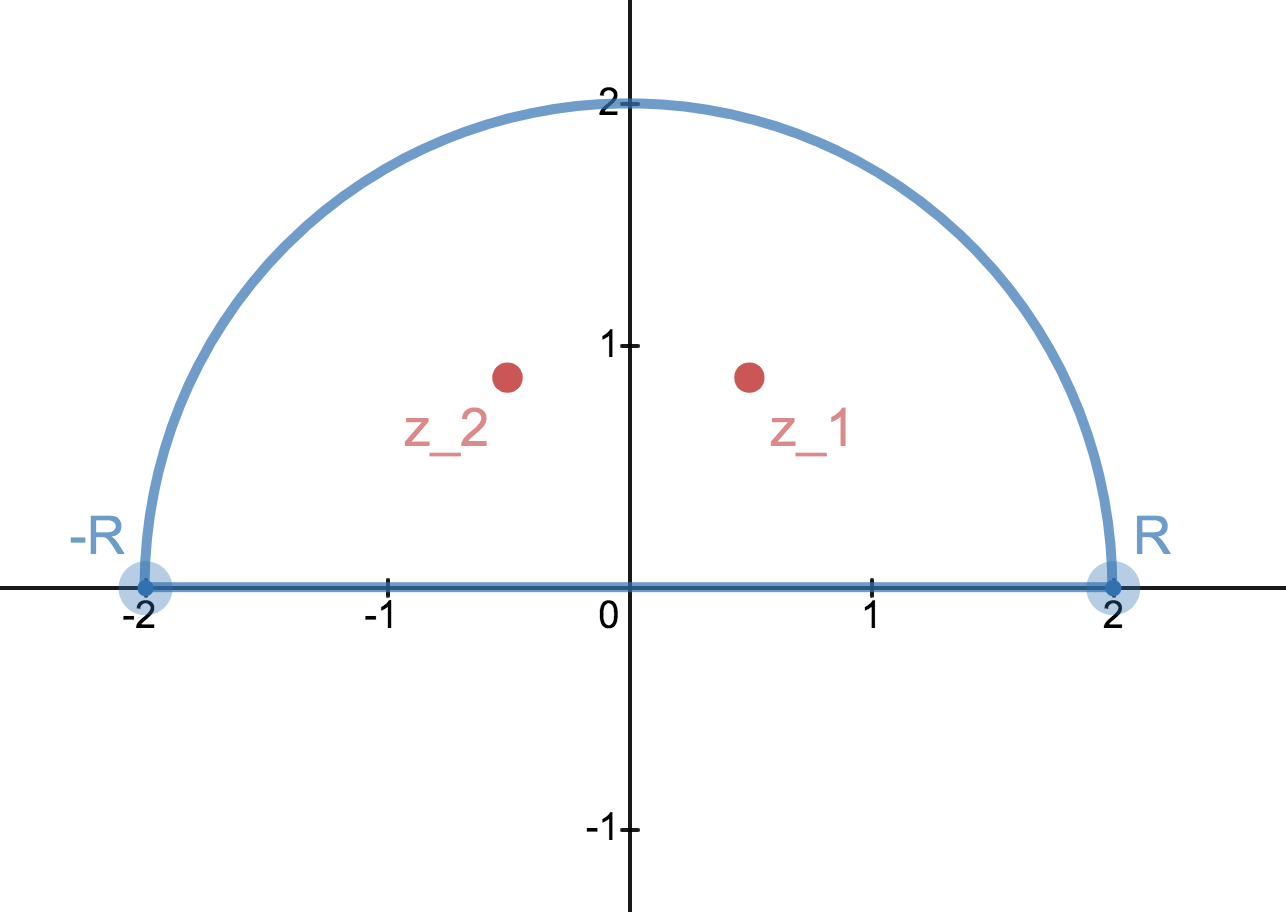
\includegraphics[width = 0.5\textwidth]{6.png}
            \caption{$\gamma$ and $z_1$ and $z_2$. Plotted in \cite{Desmos}.}
            \label{fig:fig6}
        \end{figure}
        By Residue Theorem,
        \[
            \int_{\gamma} f(z) \, \mathrm{d}z = 2\pi i \sqbrack{ \Res \paren{ f ; z_1 } + \Res \paren{ f ; z_2 } }.
        \]
        Then 
        \begin{align*}
            \Res(f;z_1) & = \lim\limits_{z \to z_1} (z - z_1) f(z) \\
            & = \left. \frac{1}{ \paren{ z + e^{\frac{\pi i}{3}} } \paren{ z - e^{-\frac{\pi i}{3}} } \paren{ z + e^{-\frac{\pi i}{3}} } } \right|_{z = z_1} \\
            & = \frac{1}{ \paren{ e^{\frac{\pi i}{3}} + e^{\frac{\pi i}{3}} } \paren{ e^{\frac{\pi i}{3}} - e^{-\frac{\pi i}{3}} } \paren{ e^{\frac{\pi i}{3}} + e^{-\frac{\pi i}{3}} } } \\
            & = \frac{1}{ \paren{ 2e^{\frac{\pi i}{3}} } \paren{ 2i \sin \paren{ \frac{\pi}{3} } } \paren{ 2 \cos \paren{ \frac{\pi}{3} } } } \\
            & = -\frac{i}{8} e^{-\frac{\pi i}{3}} \times \frac{2}{\sqrt{3}} \times \frac{2}{1} = -\frac{i e^{-\frac{\pi i}{3}} }{2\sqrt{3}},
        \end{align*}
        and 
        \begin{align*}
            \Res(f;z_2) & = \lim\limits_{z \to z_2} (z - z_2) f(z) \\
            & = \left. \frac{1}{ \paren{ z - e^{\frac{\pi i}{3}} } \paren{ z + e^{\frac{\pi i}{3}} } \paren{ z - e^{-\frac{\pi i}{3}} } } \right|_{z = z_2} \\
            & = \frac{1}{ \paren{ -e^{\frac{-\pi i}{3}} - e^{\frac{\pi i}{3}} } \paren{ -e^{\frac{-\pi i}{3}} + e^{\frac{\pi i}{3}} } \paren{ -e^{-\frac{\pi i}{3}} - e^{-\frac{\pi i}{3}} } } \\
            & = \frac{1}{ \paren{ -2 \cos \paren{ \frac{\pi}{3} } } \paren{ 2i \sin \paren{ \frac{\pi}{3} } } \paren{ -2 e^{-\frac{\pi i}{3} }  } } \\
            & = -\frac{i}{8} e^{-\frac{\pi i}{3}} \times \frac{2}{\sqrt{3}} \times \frac{2}{1} = -\frac{i e^{\frac{\pi i}{3}} }{2\sqrt{3}},
        \end{align*}
        Thus
        \begin{align*}
            \int_{\gamma} f(z) \, \mathrm{d}z & = 2\pi i \paren{ -\frac{-i e^{\frac{\pi i}{3}} }{2\sqrt{3}} -\frac{i e^{\frac{\pi i}{3}} }{2\sqrt{3}} } = \frac{(2\pi i)(-i)}{2\sqrt{3}} \paren{ e^{\frac{\pi i}{3}} + e^{-\frac{\pi i}{3}} } \\
            & = \frac{\pi}{\sqrt{3}} \times 2 \cos \paren{ \frac{\pi}{3} } = \frac{\pi}{\sqrt{3}}.
        \end{align*}
        Then we have 
        \begin{align*}
            \frac{\pi}{\sqrt{3}} & = \int_{\gamma} f(z) \, \mathrm{d}z = \int_{-R}^{R} \frac{\mathrm{d}x}{x^4 + x^2 + 1} + \underbrace{ \int_0^{\pi} \frac{i Re^{it}}{R^4e^{4it} + R^2e^{2it} + 1 } \, \mathrm{d}t }_{ \eqqcolon I(R) }.
        \end{align*}
        Note that 
        \begin{align*}
            0 & \leq |I(R)| = R \left| \int_0^{\pi} \frac{e^{it}}{R^4e^{4it} + R^2e^{2it} + 1 } \, \mathrm{d}t \right| \leq R \int_0^{\pi} \frac{1}{ \left| R^4e^{4it} + R^2e^{2it} + 1 \right| } \, \mathrm{d}t.
        \end{align*}
        By Triangle Equality, 
        \begin{align*}
            \left| R^4e^{4it} + R^2e^{2it} + 1 - 1 \right| & \leq \left| R^4e^{4it} + R^2e^{2it} + 1 \right| + |-1| \\
            \left| R^4e^{4it} + R^2e^{2it} \right| & \leq \left| R^4e^{4it} + R^2e^{2it} + 1 \right| + 1 \\
            \left| R^4e^{4it} + R^2e^{2it} + 1 \right| & \geq \left| R^2 e^{2it} \paren{ R^2 e^{2it} + 1 } \right| - 1 \\
            & = R^2 \left| R^2 e^{2it} + 1 \right| - 1.
        \end{align*}
        So 
        \begin{align*}
            |I(R)| & \leq R \int_0^{\pi} \frac{1}{ \left| R^4e^{4it} + R^2e^{2it} + 1 \right| } \, \mathrm{d}t \leq R \int_0^{\pi} \frac{ \mathrm{d}t }{ R^2 \left| R^2 e^{2it} + 1 \right| - 1 }. 
        \end{align*}
        By Triangle Inequality again, 
        \begin{align*}
            \left| R^2 e^{2it} + 1 - 1 \right| & = \left| R^2 e^{2it} + 1 \right| + |-1| \\
            \left| R^2 e^{2it} + 1 \right| & \geq \left| R^2 e^{2it} \right| - 1 \\
            & = R^2 - 1.
        \end{align*}
        Thus 
        \[
            R^2 \left| R^2 e^{2it} + 1 \right| - 1 \geq R^2 \paren{ R^2 - 1 } - 1,
        \]
        and so 
        \begin{align*}
            |I(R)| & \leq R \int_0^{\pi} \frac{ \mathrm{d}t }{ R^2 \left| R^2 e^{2it} + 1 \right| - 1 } \leq R \int_0^{\pi} \frac{ \mathrm{d}t }{ R^4 - R^2 - 1 } \\
            & = \frac{\pi R}{R^4 - R^2 - 1} \to 0
        \end{align*}
        as $R \to \infty$. Hence
        \begin{align*}
            2I & = \lim\limits_{R \to \infty} \int_{-R}^{R} \frac{\mathrm{d}x}{x^4 + x^2 + 1} = \lim\limits_{R \to \infty} \sqbrack{ \frac{\pi}{\sqrt{3}} - I(R) } = \frac{\pi}{\sqrt{3}} , \\
            I & = \frac{\pi}{2\sqrt{3}} = \frac{\pi}{2} \times \frac{\sqrt{3}}{3} = \boxed{ \frac{\pi \sqrt{3}}{6} . }
        \end{align*}
    \end{enumerate}
\end{proof}
\subsection{Problem 5}
Suppose that $D = \setb{ z | |z| < 1 }$, $H_r = \setb{ z | |z| \leq r }$ (for each $r < 1$), $\Gamma_r$ is the circle bounding $H_r$ (considered as a simple closed curve traversed in the counterclockwise direction), $f : D \to \cx$ is a function, and $f_j : D \to \cx$ is an analytic function on $D$ for each $j = 1 , 2 , \dotsc$.
\begin{enumerate}[a.]
    \item Assuming that $f$ is analytic on $D$ and $n$ is a positive integer, state the Cauchy Integral Formulas for $f(z)$ and $f^{(n)}(z)$, using the curves $\Gamma_r$.
    \item State Morera's theorem as it applies to $f$ and $D$.
    \item Using these results, show that if the sequence $\setb{ f_n }$ converges uniformly on each $D$ to a function $g$, then $g$ is also analytic on $D$ and the sequence of the derivatives of the $\setb{ f_n }$ converges uniformly to the derivative of $g$ on each $H_r$.
\end{enumerate}
\begin{proof}[Answer]
    Recall that $\setb{f_n : X \to Y}_{n=1}^{\infty}$ converges uniformly to $f : X \to Y$ if and only if 
    \[
        \lim\limits_{n \to \infty} \sup\limits_{x \in X} d_Y \paren{ f_n(x) , f(x)  } = 0.
    \]
    \begin{enumerate}[a.]
        \item For all $0 < r < 1$ and for all $n \in \n$ (yes that means $n = 0$ as well),
        \[
            f^{(n)}(z_0) = \frac{n!}{2\pi i} \int_{\Gamma_r} \frac{f(z)}{ \paren{ z - z_0 }^{n+1} } \, \mathrm{d}z
        \]
        for all $z_0 \in H_r \setminus \Gamma_r$. 
        \item If 
        \[
            \int_{\Gamma_r} f(z) \, \mathrm{d}z = 0
        \]
        for all $0 < r < 1$, then $f$ is analytic on $D$.
        \item Suppose that the sequence $\setb{ f_n }_{n=1}^{\infty}$ converges uniformly to $g$ on $D$. Since $f_n$ is analytic and thus continuous on $D$ for all $n \in \z^+$, $g$ is also continuous on $D$. By uniform convergence of the $f_n$'s, we have for all $0 < r < 1$,
        \begin{align*}
            \int_{\Gamma_r} g(z) \, \mathrm{d}z & = \int_{\Gamma_r} \sqbrack {\lim\limits_{n \to \infty} f_n(z) } \, \mathrm{d}z = \lim\limits_{n \to \infty} \int_{\Gamma_r} f_n(z) \, \mathrm{d}z \\
            & = \lim\limits_{n \to \infty} 0 = 0.
        \end{align*}
        By Morera's Theorem, $g$ is analytic on $D$. 
        
        Since $f_n$ is analytic, $f_n'$ is also analytic for all $n \in \z^+$, and for all $0 < r < 1$, $z_0 \in H_r \setminus \Gamma_r$,
        \[
            f_n'(z_0) = \frac{1}{2\pi i} \int_{\Gamma_r} \frac{f_n(z)}{ \paren{ z - z_0 }^{2} } \, \mathrm{d}z.
        \]
        Then by uniform convergence of the $f_n$'s, we have 
        \begin{align*}
            \lim\limits_{n \to \infty} f_n'(z_0) & = \lim\limits_{n \to \infty} \frac{1}{2\pi i} \int_{\Gamma_r} \frac{f_n(z)}{ \paren{ z - z_0 }^{2} } \, \mathrm{d}z =  \frac{1}{2\pi i} \int_{\Gamma_r} \lim\limits_{n \to \infty} \frac{f_n(z)}{ \paren{ z - z_0 }^{2} } \, \mathrm{d}z \\
            & = \frac{1}{2\pi i} \int_{\Gamma_r} \frac{g(z)}{ \paren{ z - z_0 }^{2} } \, \mathrm{d}z = g'(z_0)
        \end{align*}
        by Cauchy Integral Formula. Since the above is true for all $|z_0| \leq r$ for all $0 < r < 1$, $\setb{ f_n' }_{n=1}^{\infty}$ converges pointwise to $g'$ on $D$. Lastly, we show that this convergence is also uniform on each $H_r$. Since $H_r$ is compact,
        \[
            \sup\limits_{z \in H_r} \abs{ f_n'(z) - g'(z) } = \max\limits_{z \in H_r} \abs{ f_n'(z) - g'(z) },
        \]
        and so pick $z_0 \in H_r$ such that 
        \[
            \max\limits_{z \in H_r} \abs{ f_n'(z) - g'(z) } = \abs{ f_n' \paren{ z_0 } - g' \paren{z_0} }.
        \]
        Then as $f_n'$ and $g'$ are both analytic,
        \[
            \abs{ f_n' \paren{ z_0 } - g' \paren{z_0} } = \abs{ \frac{1}{2\pi i} \int_{\gamma} \frac{f_n(z)}{\paren{z-z_0}^2} \, \mathrm{d}z - \frac{1}{2\pi i} \int_{\gamma} \frac{g(z)}{\paren{z-z_0}^2} \, \mathrm{d}z }.
        \]
        where $\gamma : [0,2\pi] \to \cx$, $\gamma(t) \coloneqq z_0 + re^{it}$ for $r > 0$ small enough such that the closed disk bounded by $\gamma$ is contained in $D$. Then 
        \begin{align*}
            \abs{ \frac{1}{2\pi i} \int_{\gamma} \frac{f_n(z)}{\paren{z-z_0}^2} \, \mathrm{d}z - \frac{1}{2\pi i} \int_{\gamma} \frac{g(z)}{\paren{z-z_0}^2} \, \mathrm{d}z } & = \abs{ \frac{1}{2\pi i} \int_{\gamma} \frac{f_n(z) - g(z)}{\paren{z-z_0}^2} \, \mathrm{d}z } \\
            & = \frac{1}{2\pi} \abs{ \int_0^{2\pi} \frac{ f_n \paren{ \gamma(t) } - g \paren{ \gamma(t) } }{ \paren{ z_0 + re^{it} - z_0 }^2 } i re^{it} \, \mathrm{d}t } \\
            & \leq \frac{2 \pi}{2 \pi} \sup\limits_{0 \leq t \leq 2\pi} \frac{\abs{f_n \paren{ \gamma(t) } - g \paren{ \gamma(t) }}}{\abs{   r e^{2it}} } \\
            & = \frac{1}{r} \sup\limits_{z \in \gamma \paren{ [0,2\pi] } } \abs{ f_n(z) - g(z) }.
        \end{align*}
        Since $\gamma \paren{ [0,2\pi] } \subset D$ and $f_n$ converges to $g$ uniformly on $D$, for all $\eps > 0$ there exists $N > 0$ such that for all $n > N$,
        \[
            \frac{1}{r} \sup\limits_{z \in \gamma \paren{ [0,2\pi] } } \abs{ f_n(z) - g(z) } < \eps.
        \]
        Therefore 
        \[
            \sup\limits_{z \in H_r} \abs{ f_n'(z) - g'(z) } = 0
        \]
        and so $f_n'$ converges uniformly to $g'$ on $H_r$ for all $0 < r < 1$.
    \end{enumerate}
\end{proof}
\subsection{Problem 6}
Find a conformal map of the upper half of the open unit disk (\ita{i.e.}, from $\setb{ z | |z| < 1 \text{ and } \im(z) > 0}$ onto the entire open unit disk $\setb{ z | |z| < 1}$.
\begin{proof}[Answer]
    Let $G \coloneqq \setb{ z | |z| < 1 \text{ and } \im(z) > 0}$ and let $D$ be the open unit disk. [UNFINISHED]
\end{proof}
\newpage
\section{Spring 1993 [Answered]}
Do 5 of the 8 problems.
\subsection{Problem 1}
Find the Laurent series of the function $\ds \frac{2-z}{1+z}$ in each of the following regions:
\begin{enumerate}[(a)]
    \item $|z| < 1$
    \item $|z| > 1$.
\end{enumerate}
To get full credit, you must get the correct numerical value of the first five nonvanishing terms.
\begin{proof}[Answer]
    Let $\ds f(z) \coloneqq \frac{2-z}{1+z}$.
    \begin{enumerate}[(a)]
        \item Note that
        \begin{align*}
            f(z) & = \frac{2-z}{1+z} = \frac{2-z}{1-(-z)} = (2-z) \sum\limits_{n = 0}^{\infty} (-z)^n,
        \end{align*}
        for $|-z| < 1$, or equivalently $|z| < 1$. Then 
        \begin{align*}
            f(z) & = (2-z) \sum\limits_{n = 0}^{\infty} (-z)^n = (2 - z) \sum\limits_{n = 0}^{\infty} (-1)^n z^n \\
            & = (2 - z) \paren{ 1 - z + z^2 - z^3 + \dotsb } \\
            & = 2 - 2z + 2z^2 - 2z^3 - z + z^2 - z^3 + z^4 + \dotsb \\
            & = 2 - 3z + 3z^2 - 3z^3 + \mathcal{O} \paren{ z^4 }
        \end{align*}
        for $|z| < 1$. Continuing in this fashion, we see that for $|z| < 1$, 
        \[
            f(z) = \sum\limits_{n = 0}^{\infty} a_n z^n
        \]
        where 
        \[
            a_n = 
            \begin{cases}
                1 , & \quad n = 0 , \\
                3 (-1)^n , & \quad n \geq 1.
            \end{cases}
        \]
        \item Note that 
        \begin{align*}
            f(z) & = \frac{2-z}{1+z} = \frac{2-z}{ z \paren{ \frac{1}{z} + 1 } } \\
            & = \frac{2-z}{z} \frac{1}{ \sqbrack{ 1 - \paren{ -\frac{1}{z} } } } = \paren{ \frac{2}{z} - 1 } \sum\limits_{n = 0}^{\infty} \paren{ -\frac{1}{z} }^n
        \end{align*}
        for $\left| -\frac{1}{z} \right| < 1$, or equivalently $|z|  > 1$. Then 
        \begin{align*}
            f(z) & = \paren{ \frac{2}{z} - 1 } \sum\limits_{n = 0}^{\infty} \paren{ -\frac{1}{z} }^n \\
            & = \paren{ \frac{2}{z} - 1 } \paren{ 1 - \frac{1}{z} + \frac{1}{z^2} - \frac{1}{z^3} + \dotsb } \\
            & = \frac{2}{z} - \frac{2}{z^2} + \frac{2}{z^3} - \frac{2}{z^4} - 1 + \frac{1}{z} - \frac{1}{z^2} + \frac{1}{z^3} + \dotsb \\
            & = -1 + \frac{3}{z} - \frac{3}{z^2} + \frac{3}{z^3} + \mathcal{O} \paren{ \frac{1}{z^4} }
        \end{align*}
        for $|z| > 1$. Continuing in this fashion, we see that for $|z| > 1$,
        \[
            f(z) = \sum\limits_{n = 0}^{\infty} b_n z^{-n},
        \]
        where 
        \[
            b_n = 
            \begin{cases}
                -1 , & \quad n = 0 , \\
                3(-1)^{n+1} , & \quad n \geq 1.
            \end{cases}
        \]
    \end{enumerate}
\end{proof}
\subsection{Problem 2}
\begin{enumerate}[(a)]
    \item Describe the image of the set $D \coloneqq \setb{ re^{i \theta} \, \middle| \, 0 < r < 1 , 0 < \theta < \frac{\pi}{3} }$ under the map $z \to z^6$.
    \item Does there exists a conformal mapping of the set $D$ onto the interior of the unit circle? If not, why not? If so, find an explicit expression for one such mapping a composition of simple conformal mappings.
\end{enumerate}
\begin{proof}[Answer]
    \noindent
    \begin{enumerate}[(a)]
        \item Let $G \coloneqq \setb{ \rho e^{i \phi} \mid 0 < \rho < 1 , 0 < \phi < 2\pi }$ (note that we are not using the principal argument). We claim that $f(D) = G$. First, for $z \in f(D)$, $z = f(w)$ for some $w \in D$. Writing $w = re^{i \theta}$ for some $0 < r < 1$, $0 < \theta < \frac{\pi}{3}$, then $z = r^6 e^{i 6\theta}$. Thus $0 < \rho \coloneqq r^6 < 1$ and $0 < \phi \coloneqq 6 \theta < 2 \pi$, and so $w \in G$. Conversely, take $z = \rho e^{i \phi} \in G$ for some $0 < \rho < 1$, $0 < \phi < 2\pi$. Letting $f : \real \to \real$, $f(x) \coloneqq x^6 - \rho$, then $f$ is continuous with $f(0) = -\rho < 0$ and $f(1) = 1 - \rho > 0$. By Intermediate Value Theorem, there exists $0 < r < 1$ such that $f(r) = r^6 - \rho = 0$. Lastly, letting $\theta \coloneqq \frac{\phi}{6}$, we have $w \coloneqq re^{i \theta} \in D$ and $f(w) = z$. 
        \item UNFINISHED
    \end{enumerate}
\end{proof}
\subsection{Problem 3}
Suppose that $f$ is analytic in a connected open set $D$. Prove that any one of the following three assertions would imply that $f$ is constant.
\begin{enumerate}[(a)]
    \item $\overline{f}$ is analytic on $D$.
    \item $|f|$ is constant on $D$.
    \item $f$ is real-valued on $D$.
\end{enumerate}
($\overline{f}(z) \coloneqq \overline{f(z)}$ and $|f|(z) \coloneqq |f(z)|$ for $z \in D$.)
\begin{proof}[Answer]
    Note that if $f(x+iy) = u(x,y) + iv(x,y)$ is analytic on $D$, it satisfies the Cauchy-Riemann equations on $D$:
    \[
        u_x(x,y) = v_y(x,y) , \qquad u_y(x,y) = -v_x(x,y)
    \]
    for all $x+iy \in D$.
    \begin{enumerate}[(a)]
        \item Note that if $f(x+iy) = u(x,y) + iv(x,y)$, then $\overline{f}(x+iy) = u(x,y) -iv(x,y)$. Now, suppose that $\overline{f}$ is analytic on $D$. Then $\overline{f}$ satisfies the Cauchy-Riemann equations on $D$, and so 
        \[
            u_x(x,y) = -v_y(x,y) , \qquad u_y(x,y) = v_x(x,y)
        \]
        for all $x+iy \in D$. But since $f$ also satisfies the Cauchy-Riemann equations on $D$, we have 
        \[
            v_y(x,y) = -v_y(x,y) , \qquad v_x(x,y) = -v_x(x,y),
        \]
        or $v_x(x,y) = v_y(x,y) = 0$ for all $x+iy \in D$. Thus $v(x,y) \equiv b$ for some $b \in \real$. Similarly, 
        \[
            u_x(x,y) = -u_x(x,y) , \qquad u_y(x,y) = -u_y(x,y),
        \]
        or $u_x(x,y) = u_y(x,y) = 0$ for all $x+iy \in D$. Thus $u(x,y) \equiv a$ for some $a \in \real$, so $f(z) \equiv a + bi$. Therefore $f$ is constant on $D$.
        \item Suppose that $|f|$ is constant on $D$, then 
        \[
            u(x,y)^2 + v(x,y)^2 = R^2
        \]
        for some $R \geq 0$. Since $f$ is analytic, $u$ and $v$ are continuously differentiable on $D$, and so taking derivatives we have
        \begin{align*}
            2u(x,y) u_x(x,y) + 2v(x,y) v_x(x,y) & = 0, \\
            2u(x,y) u_y(x,y) + 2v(x,y) v_y(x,y) & = 0
        \end{align*}
        for all $x + iy \in D$. Using the Cauchy-Riemann equations, we can form a system for $u_x$ and $v_x$ (dropping the arguments of the functions for brevity):
        \begin{align*}
            u u_x + v v_x & = 0, \\
            -u v_x + v u_x & = 0.
        \end{align*}
        Writing this as a linear system, we have
        \[
            \underbrace{ 
            \begin{bmatrix}
                u & v \\
                v & -u
            \end{bmatrix}
            }_{ \eqqcolon A }
            \begin{bmatrix}
                u_x \\
                v_x
            \end{bmatrix}
            =
            \begin{bmatrix}
                0 \\
                0
            \end{bmatrix}.
        \]
        Since 
        \[
            \det(A) = -u^2 - v^2 = -R^2 \neq 0,
        \]
        the only solution to the system is $u_x = v_x = 0$. Similarly, we can form a system for $u_y$ and $v_y$ to get
        \[
            \underbrace{ 
            \begin{bmatrix}
                -v & u \\
                u & v
            \end{bmatrix}
            }_{ \eqqcolon B }
            \begin{bmatrix}
                u_y \\
                v_y
            \end{bmatrix}
            =
            \begin{bmatrix}
                0 \\
                0
            \end{bmatrix}.
        \]
        Since 
        \[
            \det(B) = -v^2 - u^2 = -R^2 \neq 0,
        \]
        $u_y = v_y = 0$. Thus $u(x,y) \equiv a$ and $v(x,y) \equiv b$ for some $a,b \in \real$, and so $f$ is constant.
        \item Suppose $f$ is real-valued on $D$. Then writing $f(x+iy) = u(x,y) + iv(x,y)$, $v(x,y) = 0$ for all $x + iy \in D$. Thus by the Cauchy-Riemann equations,
        \[
            u_x(x,y) = u_y(x,y) = 0
        \]
        for all $x + iy \in D$, and so $u$ is constant. Therefore $f$ is constant on $D$.
    \end{enumerate}
\end{proof}
\subsection{Problem 4 \texorpdfstring{\cite{Lin}}{}}
\begin{enumerate}[(a)]
    \item State Rouch\'e's theorem.
    \item Use Rouch\'e's theorem to determine the number of roots of the equation $z^7 - 5z^2 + 12 = 0$ in the annulus $1 < |z| < 2$.
\end{enumerate}
\begin{proof}[Answer]
    \noindent
    \begin{enumerate}[(a)]
        \item Suppose that $f$ and $g$ are meromorphic in a neighborhood of $\bar{B}(a;R)$ with no zeros or poles on the circle $\gamma = \partial B(a;R)$. If $Z_f,Z_{f+g}$ ($P_f,P_{f+g}$) are the number of zeros (poles) of $f$ and $f+g$ in $B(a;R)$ counted with multiplicity and if $|g(z)| < |f(z)|$ on $\gamma$, then 
        \[
            Z_f - P_f = Z_{f+g} - P_{f+g}.
        \]
        \item Let $\gamma \coloneqq \partial B(0;1)$, $f(z) \coloneqq z^7$, $g(z) \coloneqq -5z^2 + 12$. Note that on $\gamma$, $|f(z)| = 1$, and 
        \begin{align*}
            12 & = \abs{ 5z^2 - 5z^2 + 12 } \\
            & \leq \abs{ 5z^2 } + \abs{ -5z^2 + 12 } \\
            & = 5 + \abs{ -5z^2 + 12 }.
        \end{align*}
        Thus $\abs{ -5z^2 + 12 } \geq 7$, and so $|f(z)| < |g(z)|$ on $\gamma$. Since $f$ and $g$ are analytic and have no zeros on $\gamma$, $g$ and $f + g$ have the same nmber of zeros in $B(0;1)$. Since the zeros of $g$ are $\pm \sqrt{ \frac{12}{5} }$ and $\abs{ \sqrt{ \frac{12}{5} } } > 1$, $f + g$ have no zeros in $B(0;1)$. 
        
        Now, let $\sigma \coloneqq \partial B(0;2)$. Then on $\sigma$, $\abs{ f(z) } = 2^7 = 128$, while 
        \begin{align*}
            \abs{ g(z) } & = \abs{ -5z^2 + 12 } \\
            & \leq \abs{ -5z^2 } + 12 \\
            & = 5(2)^2 + 12 \\
            & = 20 + 12 \\
            & = 32.
        \end{align*}
        Thus $\abs{ g(z) } < \abs{ f(z) }$ on $\sigma$, and so $f+g$ has precisely 7 zeros on the annulus $1 < |z| < 2$. In fact, by the Fundamental Theorem of Algebra, all of the roots of $f + g$ are in this annulus.
    \end{enumerate}
\end{proof}
\subsection{Problem 5}
Evaluate $\ds \int_C z^3 \, \mathrm{d}z$, where $C$ is the path indicated in the diagram below.
\begin{center}
    \begin{tikzpicture}[node distance=1.75cm]
        \node (1+2i) {$1+2i$};
        \node (anchor) [below of = 1+2i]{};
        \node (-1+i) [left of = anchor] {$-1+i$};
        \node (3+i) [right of = anchor] {$3+i$};
        \node (0) [below right of = -1+i] {$0$};
        \node (2) [below left of = 3+i] {$2$};
        
        \draw [->] (0) -- (-1+i);
        \draw [->] (-1+i) -- (1+2i);
        \draw [->] (1+2i) -- (3+i);
        \draw [->] (3+i) -- (2);
    \end{tikzpicture}
\end{center}
\begin{proof}[Answer]
    First off, if you're gonna draw a diagram for the path you might as well draw it in the plane. Sigh.
    \begin{figure}[H]
        \centering
        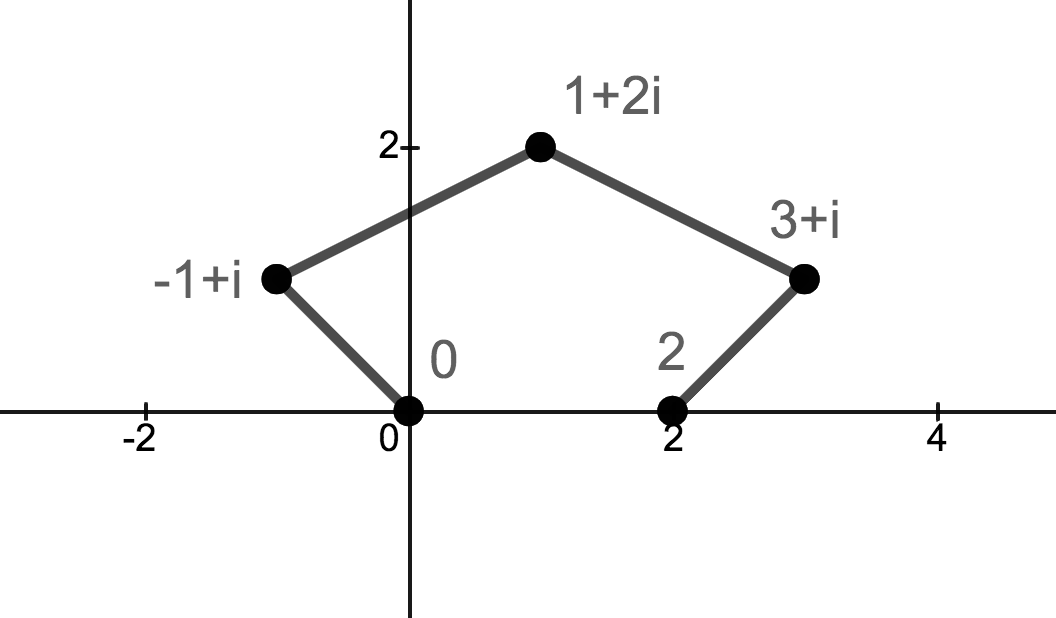
\includegraphics[width = 0.5\textwidth]{9.png}
        \caption{$C$, oriented counterclockwise. Plotted in \cite{Desmos}.}
        \label{fig:fig9}
    \end{figure}
    But it doesn't matter; $C$ is a rectifiable curve and $f(z) \coloneqq z^3$ is analytic (in fact entire) with antiderivative $F(z) = \frac{z^4}{4}$, so we can use Fundamental Theorem of Calculus:
    \begin{align*}
        \int_C z^3 \, \mathrm{d}z & = \left. \frac{z^4}{4} \right|_{z = 0}^{z = 2} = \frac{2^4 - 0^4}{4} \\
        & = \frac{16}{4} = \boxed{4.}
    \end{align*}
\end{proof}
\subsection{Problem 6}
Use residue theory to evaluate the following integrals. (Each curve has positive orientation).
\begin{enumerate}[(a)]
    \item $\ds \int_{|z| = 2} \frac{z^3 - 5z}{(z-i)^2} \, \mathrm{d}z$.
    \item $\ds \int_{|z-2| = 3} \frac{\sin z}{z^6} \, \mathrm{d}z$.
\end{enumerate}
\begin{proof}[Answer]
    Assume that the curves traverse once. 
    \begin{enumerate}[(a)]
        \item Let $C \coloneqq \setb{ z \in \cx \mid |z| = 2 }$, and let 
        \[
            I \coloneqq \int_C \frac{z^3 - 5z}{(z-i)^2} \, \mathrm{d}z.
        \]
        Letting $f(z) \coloneqq \frac{z^3 - 5z}{(z-i)^2}$, then $f$ is meromorphic with a double pole at $z = i$. Since $C$ encloses this pole, by Residue Theorem
        \[
            I = 2\pi i n(C;i) \Res(f;i) = 2\pi i \Res(f;i),
        \]
        since we take $C$ to traverse once. Then 
        \begin{align*}
            \Res(f;i) & = \left. \frac{1}{(2-1)!} \paren{ \frac{\mathrm{d}}{\mathrm{d}z} }^{2-1} \sqbrack{ (z-i)^2 f(z) } \right|_{z = i} = \left. \frac{\mathrm{d}}{\mathrm{d}z} \paren{ z^3 - 5z } \right|_{z = i} \\
            & = \left. 3z^2 - 5 \right|_{z = i} = 3\cdot i^2 - 5 \\
            & = 3(-1) - 5 = -3 - 5 \\
            & = -8.
        \end{align*}
        Then 
        \begin{align*}
            I & = 2\pi i \Res(f;i) = 2\pi i \times -8 = \boxed{ -16 \pi i . }
        \end{align*}
        \item Let $C \coloneqq \setb{ z \in \cx \mid |z-2| = 3 }$, and let
        \[
            I \coloneqq \int_C \frac{\sin z}{z^6} \, \mathrm{d}z.
        \]
        Letting $f(z) \coloneqq \frac{\sin z}{z^6}$, then $f$ is meromorphic with a pole (of order six!) at $z = 0$. Since $C$ encloses this pole, by Residue Theorem
        \[
            I  = 2\pi i n(C;0) \Res(f;0) = 2\pi i \Res(f;0),
        \]
        since we take $C$ to traverse once. Recall that if
        \[
            f(z) = \sum\limits_{n = -\infty}^{\infty} a_n (z-a)^n
        \]
        is the Laurent expansion of $f$ about $z = a$, then $\Res(f;a) \coloneqq a_{-1}$. Thus we can write
        \begin{align*}
            f(z) & = \frac{\sin z}{z^6} = \frac{1}{z^6} \sum\limits_{n = 0}^{\infty} \frac{(-1)^n z^{2n+1}}{(2n+1)!} \\
            & = \frac{1}{z^6} \sqbrack{ z - \frac{z^3}{6} + \frac{z^5}{120} - \frac{z^7}{7!} + \mathcal{O} \paren{ z^9 } } \\
            & = \frac{1}{z^5} - \frac{1}{6z^3} + \frac{1}{120z} - \frac{z}{5040} + \mathcal{O} \paren{ z^3 }.
        \end{align*}
        Thus $a_{-1} = \frac{1}{120}$, and so 
        \begin{align*}
            I & = 2\pi i \Res(f;0) = 2\pi i \times \frac{1}{120} = \boxed{ \frac{\pi i}{60} . }
        \end{align*}
    \end{enumerate}
\end{proof}
\subsection{Problem 7 \texorpdfstring{\cite{Lin}}{}}
Evaluate $\ds \int\limits_0^{\infty} \frac{\cos x}{x^2 + 1} dx$, justifying carefully the existence of any limits that arise in your computation.
\begin{proof}[Answer]
    Let 
    \[
        I \coloneqq \int_0^{\infty} \frac{\cos x}{x^2 + 1} \, \mathrm{d}x.
    \]
    Note that the integrand is even, and so we can write
    \[
        I = \frac{1}{2} \int_{-\infty}^{\infty} \frac{\cos x}{x^2 + 1} \, \mathrm{d}x.
    \]
    Let 
    \[
        f(z) \coloneqq \frac{e^{iz}}{z^2 + 1} = \frac{e^{iz}}{(z-i)(z+i)},
    \]
    then $f$ is meromorphic with simple poles at $z = \pm i$. Let $R>1$, and let $\gamma$ be the upper semicircle of radius $R$ centered at $z = 0$, oriented counterclockwise and traversing once. Then $\gamma$ encloses $z = i$, and so by Residue Theorem,
    \[
        \int_{\gamma} f(z) \, \mathrm{d}z = 2\pi i n(\gamma;i) \Res(f;i) = 2\pi i \Res(f;i).
    \]
    Then 
    \begin{align*}
        \Res(f;i) & = \lim\limits_{z \to i} \sqbrack{ (z-i) f(z) } = \lim\limits_{z \to i} \frac{e^{iz}}{z+i} = \frac{e^{-1}}{2i}.
    \end{align*}
    Thus 
    \[
        \int_{\gamma} f(z) \, \mathrm{d}z = 2\pi i \times \frac{e^{-1}}{2i} = \frac{\pi}{e},
    \]
    and so we can write
    \[
        \frac{\pi}{e} = \int_{\gamma} f(z) \, \mathrm{d}z = \underbrace{ \int_{-R}^R \frac{e^{ix}}{x^2 + 1} \, \mathrm{d}x }_{ \eqqcolon I_1(R) } + \underbrace{ \int_0^{\pi} \frac{e^{iRe^{it}}}{R^2e^{2it}+1} iRe^{it} \, \mathrm{d}t }_{ \eqqcolon I_2(R) }.
    \]
    Firstly, 
    \begin{align*}
        I_1(R) & = \int_{-R}^R \frac{e^{ix}}{x^2 + 1} \, \mathrm{d}x = \int_{-R}^R \frac{\cos x + i \sin x}{x^2 + 1} \, \mathrm{d}x \\
        & = \int_{-R}^R \frac{\cos x}{x^2 + 1} \, \mathrm{d}x + i \int_{-R}^R \frac{\sin x}{x^2 + 1} \, \mathrm{d}x.
    \end{align*}
    Since $\frac{\sin x}{x^2 + 1}$ is an odd function, $\int_{-R}^R \frac{\sin x}{x^2 + 1} \, \mathrm{d}x = 0$ for all $R \in \real$, and so 
    \[
        I_1(R) = \int_{-R}^R \frac{\cos x}{x^2 + 1} \, \mathrm{d}x.
    \]
    Then 
    \begin{align*}
        \lim\limits_{R \to \infty} I_1(R) & = \lim\limits_{R \to \infty} \int_{-R}^R \frac{\cos x}{x^2 + 1} \, \mathrm{d}x = \int_{-\infty}^{\infty} \frac{\cos x}{x^2 + 1} \, \mathrm{d}x = 2I.
    \end{align*}
    Next, we have
    \begin{align*}
        \left| I_2(R) \right| & = \left| iR \int_0^{\pi} \frac{e^{iRe^{it}}e^{it}}{R^2e^{2it}+1} \, \mathrm{d}t \right| \leq R \int_0^{\pi} \left| \frac{e^{iRe^{it}}e^{it}}{R^2e^{2it}+1} \right| \, \mathrm{d}t \\
        & = R \int_0^{\pi}  \frac{ \left| e^{iRe^{it}} \right| \left| e^{it} \right|}{\left| R^2e^{2it}+1 \right|}  \, \mathrm{d}t \leq R \int_0^{\pi}  \frac{ \left| e^{iRe^{it}} \right| }{R^2 -1 }  \, \mathrm{d}t.
    \end{align*}
    Now
    \[
        \left| e^{iRe^{it}} \right| = e^{ \re \paren{ iRe^{it} } },
    \]
    so 
    \begin{align*}
        \re \paren{ iRe^{it} } & = \re \sqbrack{ iR \paren{ \cos t + i \sin t } } = \re \paren{ iR \cos t - R \sin t } = -R \sin t.
    \end{align*}
    Thus 
    \[
        \left| e^{iRe^{it}} \right| = e^{ \re \paren{ iRe^{it} } } = e^{ -R \sin t }.
    \]
    Since $0 \leq t \leq \pi$, $0 \leq \sin t \leq 1$, and since $R > 1$, $e^{-R \sin t} \leq 1$ for all $0 \leq t \leq \pi$. Hence
    \begin{align*}
        \left| I_2(R) \right| & \leq \frac{R}{R^2 - 1} \int_0^{\pi} \left| e^{iRe^{it}} \right| \, \mathrm{d}t \leq \frac{R}{R^2 - 1} \int_0^{\pi} \, \mathrm{d}t \\
        & = \frac{\pi R}{R^2 - 1} \to 0
    \end{align*}
    as $R \to \infty$. Thus
    \begin{align*}
        2I & = \lim\limits_{R \to \infty} I_1(R) = \lim\limits_{R \to \infty} \sqbrack{ \frac{\pi}{e} - I_2(R) } = \frac{\pi}{e},
    \end{align*}
    and so 
    \[
        \int_{0}^{\infty} \frac{\cos x}{x^2 + 1} \, \mathrm{d}x = \boxed{ \frac{\pi}{2e} . }
    \]
\end{proof}
\subsection{Problem 8}
Suppose that $f$ and $g$ are entire functions such that $|f(z)| \leq |g(z)|$ for all complex numbers $z$. Prove that there is a complex number $a$ such that $f = ag$. State carefully any standard results from complex analysis that you use.
\begin{proof}[Answer]
    First, suppose that $\inv{g} \paren{ \setb{ 0 } } = \varnothing$, \ita{i.e.}, $g$ has no zeros. Then $\frac{f(z)}{g(z)}$ is defined for all $z \in \cx$, and so is entire. Then 
    \[
        \left| \frac{f(z)}{g(z)} \right| \leq 1
    \]
    for all $z \in \cx$, and so by Liouville's Theorem, $\frac{f(z)}{g(z)} \equiv a$ for some $a \in \cx$ (note that $|a| \leq 1$). Thus $f = ag$. 
    
    Now, let $z_0 \in \inv{g} \paren{ \setb{ 0 } } = \varnothing$, then $z_0$ is a singularity of $\frac{f}{g}$. We show that $z_0$ is a removable singularity. It suffices to show that 
    \[
        \lim\limits_{z \to z_0} \paren{ z - z_0 } \frac{f(z)}{g(z)} = 0.
    \]
    Since $g$ is entire and thus analytic, $\inv{g} \paren{ \setb{ 0 } }$ is a discrete set, and so there exists $r > 0$ such that for all $0 < |z-z_0| < r$, $g(z) \neq 0$. Then for $0 < |z-z_0| < r$, $\frac{f(z)}{g(z)}$ is bounded, and so
    \begin{align*}
        \lim\limits_{z \to z_0} \left| \paren{ z - z_0 }  \frac{f(z)}{g(z)} \right| & = \lim\limits_{z \to z_0} \left| z - z_0 \right| \left| \frac{f(z)}{g(z)} \right| = \lim\limits_{z \to z_0} \left| z - z_0 \right| = 0.
    \end{align*}
    Thus 
    \[
        \lim\limits_{z \to z_0} \paren{ z - z_0 } \frac{f(z)}{g(z)} = 0,
    \]
    and so $z_0$ is a removable singularity of $\frac{f}{g}$. Thus there exists $h: \cx \to \cx$ analytic (and hence entire) such that $h(z) = \frac{f(z)}{g(z)}$ for all $z \in \cx \setminus \inv{g} \paren{ \setb{ 0 } }$ (and so $h(z)g(z) = f(z)$ for all $z \in \cx)$. Now, for any $z_0 \in \inv{g} \paren{ \setb{ 0 } }$, let $\setb{ z_n }_{n = 1}^{\infty} \subset \cx \setminus \inv{g} \paren{ \setb{ 0 } } $ be a sequence converging to $z_0$, then 
    \[
        \left| h \paren{ z_n } \right| = \left| \frac{ f \paren{ z_n } }{ g \paren{ z_n } }\right| \leq 1
    \]
    for all $n \in \z^+$. Thus by continuity of $h$, 
    \[
        1 \geq \lim\limits_{n \to \infty} \left| h \paren{ z_n } \right| = \left| h \paren{ z_0 } \right|.
    \]
    Thus $|h(z)| \leq 1$ for all $z \in \cx$, and so by Liouville's Theorem $h(z) \equiv a$ for some $a \in \cx$. Thus $f = hg = ag$.
\end{proof}
\newpage
\section{Spring 1994 [Answered]}
Do 5 of 8 (include \#4 or \#7)
\subsection{Problem 1}
If $w = f(z)$ is analytic and expressed in polar coordinates $(r,\theta)$, show 
\[
    \frac{dw}{dz} = e^{-i\theta} \frac{\partial w}{\partial r}.
\]
What is the geometric interpretation of this?
\begin{proof}[Answer]
    Writing $w = f(z) = f \paren{ re^{i\theta} }$, then for all $z_0 = r_0 e^{i \theta_0}$ in the domain of $f$, 
    \[
        \lim\limits_{z \to z_0} \frac{w(z_0) - w(z)}{z - z_0} = \lim\limits_{re^{i\theta} \to r_0 e^{i \theta_0}} \frac{f \paren{ r_0 e^{i \theta_0} } - f \paren{ re^{i\theta} }}{ r_0 e^{i\theta_0} - re^{i\theta} }
    \]
    exists and is equal to $f'\paren{z_0}$. Now, take the limit $re^{i\theta} \to r_0 e^{i\theta_0}$ along the ray $\setb{ r e^{i\theta_0} \, \middle| \, r >0 }$. Then 
    \begin{align*}
        \lim\limits_{re^{i\theta} \to r_0 e^{i \theta_0}} \frac{f \paren{ r_0 e^{i \theta_0} } - f \paren{ re^{i\theta} }}{ r_0 e^{i\theta_0} - re^{i\theta} } & = \lim\limits_{r \to r_0} \frac{f \paren{ r_0 e^{i \theta_0} } - f \paren{ re^{i\theta} }}{ r_0 e^{i\theta_0} - re^{i\theta_0} } \\
        & = \frac{1}{e^{i\theta_0}} \lim\limits_{r \to r_0} \frac{f \paren{ r_0 e^{i \theta_0} } - f \paren{ re^{i\theta} }}{r_0 - r} \\
        & = e^{-i\theta_0} \lim\limits_{r \to r_0} \Bigg[ \frac{ u \paren{ r_0\cos\theta_0,r_0\sin\theta_0} - u \paren{ r\cos\theta_0,r\sin\theta_0} }{r_0 - r} \\
        & + i\frac{ v \paren{ r_0\cos\theta_0,r_0\sin\theta_0} - v \paren{ r\cos\theta_0,r\sin\theta_0} }{r_0 - r} \Bigg].
    \end{align*}
    Since $f$ is analytic, $u$ and $v$ are continuously differentiable, and so the limits evaluate to the derivatives of $u$ and $v$:
    \[
        \lim\limits_{re^{i\theta} \to r_0 e^{i \theta_0}} \frac{f \paren{ r_0 e^{i \theta_0} } - f \paren{ re^{i\theta} }}{ r_0 e^{i\theta_0} - re^{i\theta} } = e^{-i\theta_0} \paren{ \frac{\partial u}{\partial r} + i \frac{\partial v}{\partial r} } = e^{-i\theta_0} \frac{\partial f}{\partial r}.
    \]
    where the partials are evaluated at $\paren{ r_0 \cos \theta_0 , r_0 \sin \theta_0 } = r_0 e^{i\theta_0}$. Thus 
    \[
        \frac{\mathrm{d}w}{\mathrm{d}z} = e^{-i\theta} \frac{\partial w}{\partial r}.
    \]
    UNFINISHED
\end{proof}
\subsection{Problem 2}
Prove $f(z) = |z|^4$ is differentiable but not analytic at $z = 0$.
\begin{proof}[Answer]
    Let $h \in \cx$, $h \neq 0$, then 
    \begin{align*}
        \lim\limits_{h \to 0} \frac{f(0+h) - f(0)}{h} & = \lim\limits_{h \to 0} \frac{|h|^4}{h} = \lim\limits_{h \to 0} \frac{h \overline{h}|h|^2}{h} = \lim\limits_{h \to 0} \overline{h}|h|^2 = 0.
    \end{align*}
    Therefore $f'(0)$ exists and is equal to 0, thus $f$ is differentiable at $z = 0$. By way of contradiction, suppose that $f$ is analytic at $z = 0$. Then $f$ is analytic on every neighborhood of $z = 0$, in particular the open unit disk $B(0;1)$. Let $\gamma : [0,2\pi] \to \cx$, $\gamma(t) \coloneqq re^{it}$ for some $0 < r < 1$. Since $f$ is defined on all of $\cx$, then by Cauchy's Integral Formula
    \[
        \frac{1}{2\pi i} \int_{\gamma} \frac{f(z)}{z-0} \, \mathrm{d}z = n(\gamma;0)f(0) = 0.
    \]
    However,
    \begin{align*}
        \frac{1}{2\pi i} \int_{\gamma} \frac{f(z)}{z-0} \, \mathrm{d}z & = \frac{1}{2\pi} \int_{0}^{2\pi i} \frac{\abs{re^{it}}^4}{re^{it}} i re^{it} \, \mathrm{d}t = \frac{r^4}{2\pi} \int_0^{2\pi} \, \mathrm{d}t \\
        & = \frac{2\pi r^4}{2\pi} = r^4 \\
        & \neq 0 = f(0).
    \end{align*}
    Therefore $f$ is not analytic at $z = 0$.
\end{proof}
\subsection{Problem 3}
State Rouche's theorem. Use it to prove the fundamental theorem of algebra.
\begin{proof}[Answer]
    See Fall 1992, Problem 6.
\end{proof}
\subsection{Problem 4}
Show $\ds \int_0^{2\pi} \paren{ \cos \theta }^{2n} d\theta = 2\pi \binom{2n}{n} \frac{1}{2^{2n}}$.

(Hint: Write $\cos \theta = \frac{1}{2} \paren{ e^{i\theta} + e^{-i\theta} } = \frac{1}{2} \paren{ z + \inv{z} }$ for $z$ on the unit circle.
\begin{proof}[Answer]
    For $z = e^{i\theta}$, $\frac{1}{z} = e^{-i\theta}$, thus 
    \begin{align*}
        \cos \theta & = \frac{e^{i\theta}+e^{-i\theta}}{2} = \frac{z + \frac{1}{z}}{2} = \frac{z^2+1}{2z}
    \end{align*}
    for $z = e^{i\theta}$. Let $\gamma : [0,2\pi] \to \cx$, $\gamma(\theta) \coloneqq e^{i\theta}$, then for $z = e^{i\theta}$
    \begin{align*}
        \int_0^{2\pi} \paren{ \cos \theta }^{2n} \, \mathrm{d}\theta & = \int_0^{2\pi} \paren{ \frac{z^2+1}{2z} }^{2n} \, \mathrm{d}\theta = \frac{1}{2^{2n}} \int_0^{2\pi}  \frac{\paren{z^2+1}^{2n}}{z^{2n}}  \frac{i e^{i\theta}}{i e^{i\theta}} \, \mathrm{d}\theta \\
        & = \int_0^{2\pi} \frac{-i}{2^{2n}} \frac{\paren{z^2+1}^{2n}}{z^{2n+1}} i e^{i\theta} \, \mathrm{d}\theta = \frac{-i}{2^{2n}} \int_{\gamma} f(z) \, \mathrm{d}z,
    \end{align*}
    where 
    \[
        f(z) \coloneqq \frac{\paren{z^2+1}^{2n}}{z^{2n+1}}.
    \]
    Then $f$ is meromorphic with a pole of order $2n +1$ at $z = 0$. By Residue Theorem,
    \begin{align*}
        \int_0^{2\pi} \paren{ \cos \theta }^{2n} \, \mathrm{d}\theta & = \frac{-i}{2^{2n}} \int_{\gamma} f(z) \, \mathrm{d}z = \frac{-i}{2^{2n}} \times 2\pi i \Res(f;0) = \frac{2\pi}{2^{2n}} \Res(f;0).
    \end{align*}
    Thus it suffices to show that $\Res(f;0) = \binom{2n}{n}$. Then
    \begin{align*}
        \Res(f;0) & = \left. \frac{1}{(2n+1-1)!} \paren{ \frac{\mathrm{d}}{\mathrm{d}z} }^{2n+1-1} \sqbrack{ z^{2n+1} f(z) } \right|_{z = 0} \\
        & = \left. \frac{1}{(2n)!} \paren{ \frac{\mathrm{d}}{\mathrm{d}z} }^{2n} \sqbrack{ \paren{ z^2 + 1 }^{2n} } \right|_{z=0} \\
        & = \left. \frac{1}{(2n)!} \paren{ \frac{\mathrm{d}}{\mathrm{d}z} }^{2n} \sqbrack{ \sum\limits_{j = 0}^{2n} \binom{2n}{j} \paren{z^2}^{j} 1^{2n-j} } \right|_{z=0} \\
        & = \left. \frac{1}{(2n)!} \sum\limits_{j = 0}^{2n} \sqbrack{ \binom{2n}{j} \paren{ \frac{\mathrm{d}}{\mathrm{d}z} }^{2n}  \paren{z^{2j}} } \right|_{z=0}.
    \end{align*}
    Note that if $2j < 2n$, then 
    \[
        \paren{ \frac{\mathrm{d}}{\mathrm{d}z} }^{2n} \paren{z^{2j}} = 0.
    \]
    If $2j > 2n$, then $\ds \paren{ \frac{\mathrm{d}}{\mathrm{d}z} }^{2n} \paren{z^{2j}}$ will be divisible by $z$, and so vanishes upon evaluating $z = 0$. Thus the only term that survives in the sum is $2j = 2n$, or $j = n$:
    \[
        \paren{ \frac{\mathrm{d}}{\mathrm{d}z} }^{2n} \paren{z^{2n}} = (2n)!z^{2n-2n} = (2n)!.
    \]
    Thus 
    \begin{align*}
        \Res(f;0) & = \left. \frac{1}{(2n)!} \sum\limits_{j = 0}^{2n} \sqbrack{ \binom{2n}{j} \paren{ \frac{\mathrm{d}}{\mathrm{d}z} }^{2n}  \paren{z^{2j}} } \right|_{z=0} \\
        & = \left. \frac{1}{(2n)!} \binom{2n}{n} (2n)! \right|_{z=0} = \binom{2n}{n}.
    \end{align*}
    Therefore
    \[
        \int_0^{2\pi} \paren{ \cos \theta }^{2n} \, \mathrm{d}\theta = \frac{2\pi}{2^{2n}} \binom{2n}{n} .
    \]
\end{proof}
\subsection{Problem 5}
Investigate the i) absolute ii) uniform convergence of the series 
\[
    \sum\limits_{n = 0}^{\infty} \frac{z(3-z)^n}{3^{n+1}}.
\]
\begin{proof}[Answer]
    Note that 
    \[
        \sum\limits_{n = 0}^{\infty} \frac{z(3-z)^n}{3^{n+1}} = \frac{z}{3} \sum\limits_{n = 0}^{\infty} \frac{(3-z)^n}{3^{n}} = \frac{z}{3} \sum\limits_{n = 0}^{\infty} \paren{ -\frac{1}{3} }^n (z-3)^n.
    \]
    Setting $a_n \coloneqq \paren{ -\frac{1}{3} }^n$, then the radius of convergence of the series is given by 
    \begin{align*}
        R & = \lim\limits_{n \to \infty} \abs{ \frac{a_n}{a_{n+1}} } = \lim\limits_{n \to \infty} \abs{ \paren{ -\frac{1}{3} }^n \paren{ -\frac{1}{3} }^{-n-1} } \\
        & = \lim\limits_{n \to \infty} \abs{ -3 } = 3.
    \end{align*}
    Thus the series converges absolutely for $|z - 3| < 3$ and diverges for $|z - 3| > 3$. Furthermore, the series converges uniformly on $|z - 3| \leq r$ for all $0 \leq r < 3$.
\end{proof}
\subsection{Problem 6}
Euler used the following argument to show $\ds \sum\limits_{n = -\infty}^{\infty} z^n = 0$. 

First $\ds \frac{z}{1-z} = \sum\limits_{n = 1}^{\infty} z^n$.

Next $\frac{z}{z-1} = \frac{1}{1-1/z} = \sum\limits_{n = -\infty}^0 z^n$.

Adding gives 0. Explain the fallacy.
\begin{proof}[Answer]
    Note that 
    \[
        \frac{z}{1-z} = \sum\limits_{n = 1}^{\infty} z^n
    \]
    is only true for $|z|<1$, and that 
    \[
        \frac{z}{z-1} = \frac{1}{1-1/z} = \sum\limits_{n = -\infty}^0 z^n
    \]
    is only true for $\abs{\frac{1}{z}} < 1$, or equivalently for $|z| > 1$. Then the expression
    \[
        \frac{z}{1-z} + \frac{z}{z-1} = \sum\limits_{n = -\infty}^{\infty} z^n = 0
    \]
    is only valid for $\setb{ |z| < 1 } \cap \setb{ |z| > 1 } = \varnothing$, and so the statement is true for no such $z \in \cx$. 
\end{proof}
\subsection{Problem 7 \texorpdfstring{\cite{Lin}}{}}
Show $\ds \int_0^{\infty} \frac{dx}{1+x^n} = \frac{\pi}{n \sin \paren{\frac{\pi}{n}}}$, $n = 2,3,\dotsc$

Hint: Integrate over a circular sector of radius $R$, angle $\theta = \frac{2\pi}{n}$.
\begin{figure}[H]
    \centering
    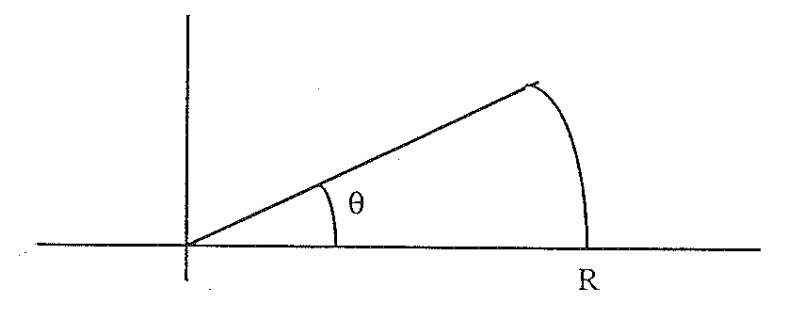
\includegraphics[width = 0.5\textwidth]{10.png}
    \caption{}
    \label{fig:fig10}
\end{figure}
\begin{proof}[Answer]
    Let $R > 0$, and let $\gamma$ be the circular sector as in Figure \ref{fig:fig10}. Then $f(z) \coloneqq \frac{1}{1+z^n}$ has simple poles at $z_k \coloneqq e^{\frac{\pi i}{n}(2k+1)}$ for $0 \leq k \leq n-1$. Since $\gamma$ encloses $z_1$, by Residue Theorem
    \begin{align*}
        \int_{\gamma} f(z) \, \mathrm{d}z & = 2\pi i \Res \paren{ f ; z_1 } = 2\pi i \Res \paren{ f ; z_1 } \\
        & = \lim\limits_{z \to z_1} \paren{ z - z_1 } f(z) = 2\pi i \lim\limits_{z \to z_1} \frac{z - z_1}{1 + z^n}.
    \end{align*}
    Evaluating $\frac{z - z_1}{1 + z^n}$ at $z = z_1$ gives $\frac{0}{0}$, so by L'Hopital's Rule we have
    \begin{align*}
        \Res \paren{ f ; z_1 } & = \lim\limits_{z \to z_1} \frac{z - z_1}{1 + z^n} = \lim\limits_{z \to z_1} \frac{1}{n z^{n-1}} \\
        & = \frac{1}{n} z_1^{1-n} = \frac{1}{n} \paren{ e^{\frac{\pi i}{n} } }^{1-n} \\
        & = \frac{1}{n} e^{\frac{\pi i}{n}} e^{\frac{-\pi in}{n}} = -\frac{1}{n} e^{\frac{\pi i}{n}}.
    \end{align*}
    Break up $\gamma$ into three pieces: $\gamma_1$ being the line segment from $0$ to $R$ along the real axis, $\gamma_2$ being the circular arc from $R$ to $Re^{\frac{2\pi i}{n}}$, and $\gamma_3$ being the radial line segment from $Re^{\frac{2\pi i}{n}}$ to $0$. Then
    \begin{align*}
        -\frac{2\pi i}{n} e^{\frac{\pi i}{n}} & = 2\pi i \Res \paren{ f ; z_1 } = \int_{\gamma} f(z) \, \mathrm{d}z \\
        & = \int_{\gamma_1} f(z) \, \mathrm{d}z + \int_{\gamma_2} f(z) \, \mathrm{d}z + \int_{\gamma_3} f(z) \, \mathrm{d}z.
    \end{align*}
    Firstly, 
    \[
        \int_{\gamma_1} f(z) \, \mathrm{d}z = \int_{-R}^R \frac{\mathrm{d}x}{1+x^n}.
    \]
    Next, take $\gamma_2(t) \coloneqq Re^{it}$, $0 \leq t \leq \frac{2\pi}{n}$. Then 
    \begin{align*}
        \abs{ \int_{\gamma_2} f(z) \, \mathrm{d}z } & = \abs{ \int_0^{\frac{2\pi }{n}} \frac{1}{1+\paren{Re^{it} }^n} iRe^{it} \, \mathrm{d}t } \leq R \int_0^{\frac{2\pi }{n}} \frac{ \mathrm{d}t }{ \abs{ 1+\paren{Re^{it} }^n } } \\
        & \leq R \int_0^{\frac{2\pi }{n}} \frac{ \mathrm{d}t }{ R^n - 1 } = \frac{2\pi R}{n\paren{R^n-1}} \\
        & \to 0
    \end{align*}
    as $R \to \infty$, since $n > 1$. Now, take $\gamma_3(t) \coloneqq te^{\frac{2\pi i}{n}}$, $R \leq t \leq 0$. Then 
    \begin{align*}
        \int_{\gamma_3} f(z) \, \mathrm{d}z & = -\int_0^R \frac{1}{1+\paren{te^{\frac{2\pi i}{n}}}^n} e^{\frac{2\pi i}{n}} \, \mathrm{d}t = -e^{\frac{2\pi i}{n}} \int_0^R \frac{ \mathrm{d}t }{ 1+t^n }.
    \end{align*}
    Thus 
    \begin{align*}
        \lim\limits_{R \to \infty} \paren{ -\frac{2\pi i}{n} e^{\frac{\pi i}{n}} } & = \lim\limits_{R \to \infty} \sqbrack{ \int_{\gamma_1} f(z) \, \mathrm{d}z + \int_{\gamma_2} f(z) \, \mathrm{d}z + \int_{\gamma_3} f(z) \, \mathrm{d}z }  \\
        -\frac{2\pi i}{n} e^{\frac{\pi i}{n}} & = \int_0^{\infty} \frac{\mathrm{d}x}{1+x^n} + 0 - e^{\frac{2\pi i}{n}} \int_0^{\infty} \frac{ \mathrm{d}x }{ 1+x^n } \\
        \int_0^{\infty} \frac{ \mathrm{d}x }{ 1+x^n } & = -\frac{2\pi i}{n} e^{\frac{\pi i}{n}} \times \frac{1}{1-e^{\frac{2\pi i}{n}}} \\
        & = \frac{2\pi i}{n} \frac{1}{e^{-\frac{\pi i}{n}} \paren{ e^{\frac{2\pi i}{n}} - 1 } } \\
        & = \frac{2\pi i}{n \paren{ e^{\frac{\pi i}{n}} - e^{\frac{-\pi i}{n}} }} \\
        & = \boxed{ \frac{\pi}{n \sin\paren{\frac{\pi}{n}}} }.
    \end{align*} 
\end{proof}
\subsection{Problem 8}
Suppose $f : \cx \to \cx$ is analytic and $\re(f)$ is bounded. Show $f$ is constant.
\begin{proof}[Answer]
    Let $f : \cx \to \cx$ be analytic (thus entire). Write $f(z) = f(x+iy) = u(x,y) + iv(x,y)$, and suppose that $u$ is bounded. Then there exists $M > 0$ such that 
    \[
        \abs{ u(x,y) } \leq M
    \]
    for all $x+iy \in \cx$. Then
    \begin{align*}
        \abs{ e^{f(z)} } & = e^{\re\paren{f(z)}} = e^{u(x,y)} \leq e^M.
    \end{align*}
    for all $x+iy \in \cx$. Since the composition of analytic functions is analytic, $e^{f(z)}$ is a bounded entire function. By Liouville's Theorem, $e^{f(z)} = c$ for all $z \in \cx$, for some fixed $c \in \cx$. Then 
    \begin{align*}
        \frac{\mathrm{d}}{\mathrm{d}z} \sqbrack{ e^{f(z)} } & = \frac{\mathrm{d}}{\mathrm{d}z} \paren{ c } \\
        e^{f(z)} f'(z) & = 0.
    \end{align*}
    Since $e^{f(z)} \neq 0$ for all $z \in \cx$, $f'(z) = 0$ for all $z \in \cx$ and so $f$ is constant.
\end{proof}
\newpage
\section{Spring 2014 [Answered]}
Solve 3 of the 4 problems in both Parts 1 and 2. Each problem is worth 10 points. This exam will test the extent of your knowledge and the clarity of your mathematical writing, so be sure to show all your working and justify all your steps. You must pass \textbf{both} parts in order to pass the exam. 
\subsection{Problem 1}
Given $a > 0$, $b > 0$, prove that 
\[
    \int_{-\infty}^{\infty} \frac{\cos bx}{a^2 + x^2} dx = \pi \inv{ \paren{ a e^{ab} } }.
\]
\begin{proof}[Answer]
    Let 
    \begin{align*}
        I & \coloneqq \int_{-\infty}^{\infty} \frac{\cos(bx)}{a^2 + x^2} \, \mathrm{d}x = \frac{1}{a^2} \int_{-\infty}^{\infty} \frac{\cos(bx)}{1 + \paren{ \frac{x}{a} }^2} \, \mathrm{d}x = \frac{1}{a} \int_{-\infty}^{\infty} \frac{\cos(aby)}{1+y^2} \, \mathrm{d}y.
    \end{align*}
    Now, let 
    \[
        f(z) \coloneqq \frac{e^{abiz}}{1 + z^2} = \frac{e^{abiz}}{(z-i)(z+i)},
    \]
    then $f$ is meromorphic with simple poles at $z = \pm i$. Let $R > 0$, and let $\gamma$ be the upper semicircle of radius $R$ centered at the origin, oriented counterclockwise. Then by Residue Theorem,
    \[
        \int_{\gamma} f(z) \, \mathrm{d}z = 2\pi i n(\gamma;i) \Res(f;i) = 2\pi i \Res(f;i).
    \]
    So
    \begin{align*}
        \Res(f;i) & = \lim\limits_{z \to i} (z-i) f(z) = \left. \frac{e^{abiz}}{z+i} \right|_{z = i} = \frac{e^{-ab}}{2i},
    \end{align*}
    hence
    \[
        \pi e^{-ab} = \int_{\gamma} f(z) \, \mathrm{d}z = \int_{-R}^R \frac{e^{iaby}}{1+y^2} \, \mathrm{d}y + \int_{0}^{\pi} \frac{ \exp \paren{abRe^{it} } }{ 1 + R^2 e^{2it} } iRe^{it} \, \mathrm{d}t.
    \]
    For the first integral, we have
    \[
        \int_{-R}^R \frac{e^{iaby}}{1+y^2} \, \mathrm{d}y = \int_{-R}^R \frac{\cos(aby) + i \sin(aby)}{1+y^2} \, \mathrm{d}y = \int_{-R}^R \frac{\cos(aby)}{1+y^2} \, \mathrm{d}y + i \int_{-R}^R \frac{\sin(aby)}{1+y^2} \, \mathrm{d}y.  
    \]
    Since $\frac{\sin(aby)}{1+y^2}$ is an odd function,
    \[
        \int_{-R}^R \frac{\sin(aby)}{1+y^2} \, \mathrm{d}y = 0,
    \]
    and so 
    \[
        \int_{-R}^R \frac{e^{iaby}}{1+y^2} \, \mathrm{d}y = \int_{-R}^R \frac{\cos(aby)}{1+y^2} \, \mathrm{d}y.
    \]
    Then 
    \[
        \lim\limits_{R \to \infty} \int_{-R}^R \frac{e^{iaby}}{1+y^2} \, \mathrm{d}y = \lim\limits_{R \to \infty} \int_{-R}^R \frac{\cos(aby)}{1+y^2} \, \mathrm{d}y = a I.
    \]
    For the second integral, note that
    \begin{align*}
        \abs{ \int_{0}^{\pi} \frac{ \exp \paren{abRe^{it} } }{ 1 + R^2 e^{2it} } iRe^{it} \, \mathrm{d}t } & \leq R \int_0^{\pi} \frac{ \abs{ \exp \paren{ abRe^{it} } } }{ \abs{ 1 + R^2 e^{2it} } } \, \mathrm{d}t \leq R \int_0^{\pi} \frac{ e^{ \re \paren{ ab Re^{it} } } }{ R^2 - 1 } \, \mathrm{d}t \\
        & = \frac{R}{R^2 - 1} \int_0^{\pi} \exp \sqbrack{ abR \cos(t) } \, \mathrm{d}t \leq \frac{\pi R}{R^2 - 1} e^{abR} \\
        & \to 0
    \end{align*}
    as $R \to \infty$. Therefore
    \begin{align*}
        \lim\limits_{R \to \infty} \pi e^{-ab} & = \lim\limits_{R \to \infty} \int_{\gamma} f(z) \, \mathrm{d}z \\
        \pi e^{-ab} & = aI + 0 \\
        I & = \boxed{ \pi \inv{ \paren{ ae^{ab} } }. }
    \end{align*}
\end{proof}
\subsection{Problem 2 \texorpdfstring{\cite{Conway}}{}}
Let $f(z)$ be an analytic function in the unit disk
\[
    D = \setb{ z \in \cx : |z| < 1 }.
\]
Suppose that $f(0) = 0$ and $\abs{ f(z) } \leq 1$ for $z \in D$. Prove Schwarz' Lemma, namely:
\begin{enumerate}[(a)]
    \item $\abs{ f(z) } \leq \abs{ z }$ for $z \in D$, 
    \item $\abs{ f'(0) } \leq 1$, and
    \item if there exists $z_0 \in D \setminus \setb{ 0 }$ such that $\abs{ f \paren{ z_0 } } = \abs{ z_0 }$, then $f(z) = e^{i \theta} z$, for some $\theta \in \real$.
\end{enumerate}
(Hint: Consider the function $g(z) = f(z)/z$.)
\begin{proof}[Answer]
    Let $g(z) \coloneqq \frac{f(z)}{z}$ for $z \in D$, then $g$ is analytic on $0 < |z| < 1$, and since
    \begin{align*}
        \lim\limits_{z \to 0} z g(z) & = \lim\limits_{z \to 0} f(z) = f(0) = 0,
    \end{align*}
    $g$ has a removable singularity at $z = 0$, and so there exists $h : D \to \cx$ analytic such that $h(z) = g(z)$ for all $0 < |z| < 1$ and 
    \[
        h(0) = \lim\limits_{z \to 0} g(z) = f'(0).
    \]
    Then for all $0 < |z| < 1$, 
    \[
        \abs{ h(z) } = \abs{ \frac{f(z)}{z} } \leq \abs{ \frac{1}{z} }.
    \]
    Let $0 < r < 1$, then $h$ is analytic on $\bar{B}(0;r)$, so by Maximum Modulus Principle, 
    \begin{align*}
        \max\limits_{z \in \bar{B}(0;r)} \abs{ h(z) } & = \max\limits_{z \in \partial B(0;r)} \abs{ h(z) } \leq \max\limits_{z \in \partial B(0;r)} \abs{ \frac{1}{z} } = \frac{1}{r}.
    \end{align*}
    Thus $\abs{ h(z) } \leq \frac{1}{r}$ for all $|z| < r$, for $0 < r < 1$. Taking $r \to 1$ gives us 
    \[
        \abs{ h(z) } = \abs{ \frac{f(z)}{z} } \leq 1
    \]
    for all $0 < |z| < 1$, and so $\abs{ f(z) } \leq |z|$. Since $f(0) = 0$, $\abs{ f(z) } \leq |z|$ for all $z \in D$.
    
    Let $0 < r < 1$, $\gamma : [0,2\pi] \to \cx$ given by $\gamma(t) \coloneqq re^{it}$. Since $f$ is analytic, by Cauchy's Integral Formula
    \begin{align*}
        n(\gamma;0)f'(0) & = \frac{1!}{2\pi i} \int_{\gamma} \frac{f(w)}{(w-0)^{1+1}} \, \mathrm{d}w \\
        f'(0) & = \frac{1}{2\pi i} \int_0^{2\pi} \frac{ f \paren{ re^{it} } }{ r^2 e^{2it} } ire^{it} \, \mathrm{d}t \\
        & = \frac{1}{2\pi r} \int_0^{2\pi} f \paren{ re^{it} } e^{-it} \, \mathrm{d}t.
    \end{align*}
    Then 
    \begin{align*}
        \abs{ f'(0) } & = \frac{1}{2\pi r} \abs{ \int_0^{2\pi} f \paren{ re^{it} }  e^{-it} \, \mathrm{d}t } \leq \frac{1}{2\pi r} \int_0^{2\pi} \abs{ f \paren{ re^{it} }  e^{-it} } \, \mathrm{d}t \\
        & = \frac{1}{2\pi r}\int_0^{2\pi} \abs{ f \paren{ re^{it} } } \, \mathrm{d}t \leq \frac{1}{2\pi r} 2\pi \sup\limits_{w \in \gamma \paren{ [0,2\pi] }} \abs{ f(w) } \\
        & \leq \frac{1}{r}.
    \end{align*}
    Thus
    \begin{align*}
        \lim\limits_{r \to 1} \abs{ f'(0) } & \leq \lim\limits_{r \to 1} \frac{1}{r} \\
        \abs{ f'(0) } & \leq 1.
    \end{align*}
    Lastly, suppose that there exists $z_0 \in D \setminus \setb{ 0 }$ such that $\abs{ f \paren{ z_0 } } = \abs{ z_0 }$. Then
    \begin{align*}
        \abs{ h \paren{ z_0 } } & = \abs{ \frac{f \paren{ z_0 } }{z_0} } = \frac{\abs{ f \paren{ z_0 } }}{\abs{ z_0 }} \\
        & = \frac{\abs{ z_0 }}{\abs{ z_0 }} = 1.
    \end{align*}
    Since $\abs{ h(z) } \leq 1$ for all $z \in D$, $h$ assumes its maximum in $D$, so by Maximum Modulus Theorem $h$ is constant. Thus $h(z) = w$ for some $|w| = 1$ Writing $w = e^{i\theta}$ for some $\theta \in \real$, we have
    \begin{align*}
        e^{i\theta} & = h(z) = \frac{f(z)}{z} , \\
        f(z) & = e^{i\theta} z
    \end{align*}
    for all $0 < |z| < 1$. Since $f(0) = 0 = e^{i\theta} \cdot 0$, $f(z) = e^{i\theta} z$ for all $z \in D$.
\end{proof}
\subsection{Problem 3}
Show that all the zeros of 
\[
    p(z) = 3z^3 - 2z^2 + 2iz - 8
\]
lie in the annulus $\setb{z \in \cx : 1 < |z| < 2}$.
\begin{proof}[Answer]
    Let $\gamma \coloneqq \setb{ |z| = 1 }$, $f(z) \coloneqq 3z^3 + 2iz = z \paren{3z^2 + 2i}$, $g(z) \coloneqq -2z^2 - 8$. Then $f$ and $g$ are analytic on $\bar{B}(0;1)$, and $f + g = p$. By the Fundamental Theorem of Algebra, $f$ has three zeros, and the zeros are either $0$ or have magnitude $\sqrt{\frac{2}{3}}$. $g$ has simple roots at $z = \pm 2i$, thus $f$ and $g$ are not zero on $\gamma$. Lastly, for all $z \in \gamma$,
    \begin{align*}
        \abs{ f(z) } & = \abs{z} \abs{3z^2 + 2i} = \abs{3z^2 + 2i} \\
        & \leq \abs{3z^2} + \abs{2i} = 3 \cdot1^2 + 2 \\
        & = 3 + 2 = 5,
    \end{align*}
    while
    \begin{align*}
        \abs{ g(z) } & = \abs{ -2z^2 - 8} \geq \abs{-8} - \abs{2z^2} \\
        & = 8 - 2\cdot1^2 = 8 - 2 \\
        & = 6 > 5.
    \end{align*}
    Therefore $|f(z)| < |g(z)|$ on $\gamma$. By Rouche\'s Theorem, $g$ and $p$ have the same number of zeros in $B(0;1)$ counted with multiplicity. Since the zeros of $g$ are $\pm 2i \notin B(0;1)$, $p$ has no zeros in $B(0;1)$.
    
    Now, let $\sigma = \setb{ |z| = 2 }$, $f(z) \coloneqq 3z^3 - 8$, $g(z) \coloneqq 2iz - 2z^2 - 2z(i-z)$. Then $f$ and $g$ are analytic on $\bar{B}(0;2)$, and $f + g = p$. By the Fundamental Theorem of Algebra, $f$ has three zeros counted with multiplicity, and those zeros lie on 
    \begin{align*}
        |z| & = \paren{ \frac{8}{3} }^{\frac{1}{3}} = \frac{2}{3^{\frac{1}{3}}} < 2,
    \end{align*}
    and so $f$ has no zeros on $\sigma$, and are contained in $B(0;2)$. Furthermore, the zeros of $g$ are $z = 0$ and $z = i$, so $g$ has no zeros on $\sigma$. Lastly, for $z \in \sigma$, 
    \begin{align*}
        \abs{ g(z) } & = \abs{ 2z(i-z) } = 2\abs{z}\abs{i-z} \\
        & \leq 2\cdot2 \paren{ \abs{i} + \abs{-z} } = 4 \paren{1 + 2} \\
        & = 4 \cdot 3 = 12,
    \end{align*}
    while
    \begin{align*}
        \abs{ f(z) } & = \abs{ 3z^3 - 8 } \geq \abs{ 3z^3 } - \abs{ 8 } \\
        & = 3 \cdot 2^3 - 8 = 3 \cdot 8 - 8 \\
        & = 24 - 8 = 16 \\
        & > 12.
    \end{align*}
    Thus $|g(z)| < |f(z)|$ for all $z \in \sigma$. By Rouche\'s Theorem, $p$ and $f$ have the same number of zeros counted with multiplicity in $B(0;2)$. Thus $p$ has three zeros in $B(0;2)$. Since $p$ has no zeros in $B(0;2)$, all of the zeros of $p$ lie in the annulus $1 < |z| < 2$.
\end{proof}
\subsection{Problem 4}
Does there exist an analytic function $f$ defined on the unit disk $\setb{ z \in \cx : |z| < 1 }$ such that 
\[
    f \paren{ \frac{1}{n} } = 
    \begin{cases}
        \frac{1}{n} , & \quad n = 2 , 4 , 6 , \dotsc \\
        \frac{1}{n+1} , & \quad n = 3 , 5 , 7 , \dotsc 
    \end{cases}
\]
holds?
\begin{proof}[Answer]
    Suppose such an analytic function $f : D \to \cx$ does exist. Then for all $n \in \z^+$,
    \begin{align*}
        f \paren{ \frac{1}{2n} } & = \frac{1}{2n}, \\
        f \paren{ \frac{1}{2n+1} } & = \frac{1}{2(n+1)}.
    \end{align*}
    By continuity of $f$,
    \begin{align*}
        f(0) & = \lim\limits_{n \to \infty} f \paren{ \frac{1}{2n} } \\
        & = \lim\limits_{n \to \infty} \frac{1}{2n} \\
        & = 0.
    \end{align*}
    UNFINISHED
\end{proof}
\newpage
\section{Fall 2014 [Answered]}
Do \textbf{only} 3 problems from each part of the exam. Start each problem on a new sheet of paper. Write on one side only and avoid the edges since the exams will be copied for grading. Each problem is worth 10 points; when problems have parts, the parts are equally weighted unless the explicit is indicated.

\textbf{Be sure to justify all of your answers by citing theorems or showing computations. Details matter; the right idea or even the right answer will not get full credit without clear justification.}

Notation: $\mathbb{D}$ will denote the open unit disk.
\subsection{Problem 1}
Suppose that 
\[
    f(z) = \int_0^1 \frac{dt}{(1+tz)}
\]
for every $z \in \mathbb{D}$. Find a power series that represents $f$ in $\mathbb{D}$.
\begin{proof}[Answer]
    Note that since $0 \leq t \leq 1$,
    \[
        \frac{1}{1+tz} = \sum\limits_{n = 0}^{\infty} \paren{-tz}^n = \sum\limits_{n = 0}^{\infty} (-1)^n t^n z^n.
    \]
    The radius of convergence of the above sum is 
    \begin{align*}
        R & = \lim\limits_{n \to \infty} \abs{ \frac{(-1)^n}{n+1} \frac{n+2}{(-1)^{n+2}} } = \lim\limits_{n \to \infty} \frac{n+2}{n+1} = 1,
    \end{align*}
    so the sum converges uniformly on every compact $K \subset \mathbb{D}$. Then 
    \begin{align*}
        f(z) & = \int_0^1 \frac{\mathrm{d}t}{(1+tz)} = \int_0^1 \sqbrack{ \sum\limits_{n = 0}^{\infty} (-1)^n t^n z^n } \, \mathrm{d}t \\
        & = \sum\limits_{n = 0}^{\infty} (-1)^n z^n \int_0^1 t^n \, \mathrm{d}t = \sum\limits_{n = 0}^{\infty} \frac{(-1)^n}{n+1} z^n
    \end{align*}
    for all $z \in K$ for every compact $K \subset \mathbb{D}$.
\end{proof}
\subsection{Problem 2 \texorpdfstring{\cite{Nguyen}}{}}
Suppose that $f_1$, $f_2$ are non-constant analytic functions on $\mathbb{D}$. Define $g = \abs{f_1} + \abs{f_2}$ on $\mathbb{D}$. Prove that $g$ does not attain a local maximum at any point of $\mathbb{D}$.
\begin{proof}[Answer]
    By Maximum Modulus Principle, $f_1$ and $f_2$ do not attain a maximum at any point of $\mathbb{D}$. Note that $g$ itself cannot be constant on $\mathbb{D}$: since $\abs{ f_j(z) } \geq 0$ for all $z \in \mathbb{D}$ and $f_j$ is not constant on $\mathbb{D}$, if $g$ is constant then $\abs{ f_j }$ must be constant on $\mathbb{D}$. This would force $f_j$ to be constant, which contradicts what is given. 
    
    By way of contradiction, suppose that $g$ does attain a local maximum at $z_0 \in \mathbb{D}$. Write
    \[
        f_j \paren{ z_0 } = r_j e^{i \theta_j}
    \]
    where $-\pi < \theta_j \leq \pi$, $j = 1,2$. Then the maximum of $g$ on $\mathbb{D}$ is 
    \[
        g \paren{ z_0 } = r_1 + r_2.
    \]
    Define $h : \mathbb{D} \to \cx$ by
    \[
        h(z) \coloneqq e^{-i \theta_1} f_1(z) + e^{-i \theta_2} f_2(z).
    \]
    Note that $h$ is analytic, and for all $z \in \mathbb{D}$,
    \begin{align*}
        \abs{ h(z) } & = \abs{ e^{-i \theta_1} f_1(z) + e^{-i \theta_2} f_2(z) } \leq \abs{ e^{-i \theta_1} f_1(z) } + \abs{ e^{-i \theta_2} f_2(z) } \\
        & = \abs{ f_1(z) } + \abs{ f_2(z) } = g(z) \\
        & \leq g \paren{ z_0 } = r_1 + r_2 \\
        & = h \paren{ z_0 } .
    \end{align*}
    By Maximum Modulus Theorem, $h$ must be constant, with fixed value $r_1 + r_2$. Then for all $z \in \mathbb{D}$,
    \begin{align*}
        r_1 + r_2 & = \abs{ h(z) } \leq \abs{ f_1(z) } + \abs{ f_2(z) } \\
        & = g(z) \leq r_1 + r_2,
    \end{align*}
    and so $g$ is constant on $\mathbb{D}$, a contradiction. Therefore $g$ does not attain a local maximum on $\mathbb{D}$.
\end{proof}
\subsection{Problem 3}
Find a 1-1 analytic function that maps the quarter disk $\setb{ z = x + iy : |z| < 1, x > 0 , y > 0 }$ onto $\mathbb{D}$.
\begin{proof}[Answer]
    UNANSWERED
\end{proof}
\subsection{Problem 4 \texorpdfstring{\cite{Leon}}{}}
Show that the polynomial $z^5 - 6z + 3$ has 5 distinct complex roots and that exactly 3 are real.
\begin{proof}[Answer]
    To find the real roots of $p(z) \coloneqq z^5 - 6z + 3$, first we find the critical points of $p$. Set $p'(z) = 0$:
    \begin{align*}
        p'(z) & = 5z^4 - 6 = 0 \\
        z & = \pm \sqrt[4]{\frac{6}{5}}.
    \end{align*}
    Note that 
    \begin{align*}
        p'(0) & = -6 < 0, \\
        p'(\pm2) & = 5\cdot(\pm2)^4 - 6 = 5 \cdot 16 - 6 \\
        & = 80 - 6 = 74 \\ 
        & > 0.
    \end{align*}
    Thus $p$ is decreasing on $\paren{ -\sqrt[4]{\frac{6}{5}} , +\sqrt[4]{\frac{6}{5}} }$, and increasing on the interior of the complement of that interval. Note that
    \begin{align*}
        p \paren{ +\sqrt[4]{\frac{6}{5}} } & = \paren{ \frac{6}{5} }^{\frac{5}{4}} - 6 \paren{ \frac{6}{5} }^{\frac{1}{4}} + 3 \\
        & = \paren{ \frac{6}{5} }^{\frac{1}{4}} \paren{ \frac{6}{5} - 6 } + 3 \\
        & = -\sqrt[4]{\frac{6}{5}} \cdot \frac{24}{5} + 3.
    \end{align*}
    Since $\frac{24}{5} > 3$ and $\sqrt[4]{\frac{6}{5}} > 1$, $p \paren{ +\sqrt[4]{\frac{6}{5}} } < 0$, while
    \begin{align*}
        p \paren{ -\sqrt[4]{\frac{6}{5}} } & = -\paren{ \frac{6}{5} }^{\frac{5}{4}} + 6 \paren{ \frac{6}{5} }^{\frac{1}{4}} + 3 \\
        & = \paren{ \frac{6}{5} }^{\frac{1}{4}} \paren{ -\frac{6}{5} + 6 } + 3 \\
        & = \sqrt[4]{\frac{6}{5}} \cdot \frac{24}{5} + 3 \\
        & > 0.
    \end{align*}
    Then since $p$ is decreasing on $\paren{ -\sqrt[4]{\frac{6}{5}} , +\sqrt[4]{\frac{6}{5}} }$, by Intermediate Value Theorem $p$ must have a root on $\paren{ -\sqrt[4]{\frac{6}{5}} , +\sqrt[4]{\frac{6}{5}} }$. Since 
    \[
        \lim\limits_{x \to +\infty} p(x) = + \infty , \qquad \lim\limits_{x \to -\infty} p(-x) = - \infty ,
    \]
    $p$ must eventually have a root $x_1 > \sqrt[4]{\frac{6}{5}}$ and a root $x_2 < -\sqrt[4]{\frac{6}{5}}$. Therefore $p$ has 3 real roots, all distinct. 
    
    By Fundamental Theorem of Algebra, $p$ must have 5 complex roots, and so the remaining roots are nonreal and come in conjugate pairs. Thus $p$ has 5 distinct complex roots, 3 of which are real.
\end{proof}
\subsection{Problem 5}
Let $f(z) = \inv{z} \inv{ (z-\pi) } \inv{ (z-e) }$. Find the partial fraction decomposition for $f$. $f$ has three Laurent series representations corresponding to 3 annuli centered at the origin. Describe the annuli and find the Laurent series for each one. Be sure to justify your conclusions.
\begin{proof}[Answer]
    UNANSWERED
\end{proof}
\newpage
\section{Spring 2015}
Answer three complete questions in each of the two sections. Each problem is worth 10 points. You must fully justify all of your answers in order to get full credit.
\subsection{Problem 1}
Prove that 
\[
    \int_0^{\infty} \frac{x^{s-1} dx}{1+x^4} = \frac{\pi}{8 \sin \frac{\pi s}{4}} , \quad 0 < s < 4.
\]
\begin{proof}[Answer]
    
\end{proof}
\subsection{Problem 2}
Describe the image of the upper half-plane by the analytic mapping 
\[
    w = \log(1-z^2).
\]
\begin{proof}[Answer]
    We write the mapping as a composition of 4 maps: 
    \[
        f \coloneqq f_4 \circ f_3 \circ f_2 \circ f , 
    \]
    where 
    \begin{align*}
        f_1(z) & \coloneqq z^2 , \\ 
        f_2(z) & \coloneqq -z , \\ 
        f_3(z) & \coloneqq 1 + z , \\ 
        f_4(z) & \coloneqq \log(z) , 
    \end{align*}
    where $\log$ is the principal branch of the logarithm. Let $H$ denote the upper half-plane. 
    
    First, note that $f_1(H)$ is $\cx \setminus \setb{ x \in \real \, \middle| \, x \geq 0 }$, since no nonnegative real number is the square of a non-real complex number. 
    \begin{figure}[H]
        \begin{subfigure}{0.45\textwidth}
            \centering
            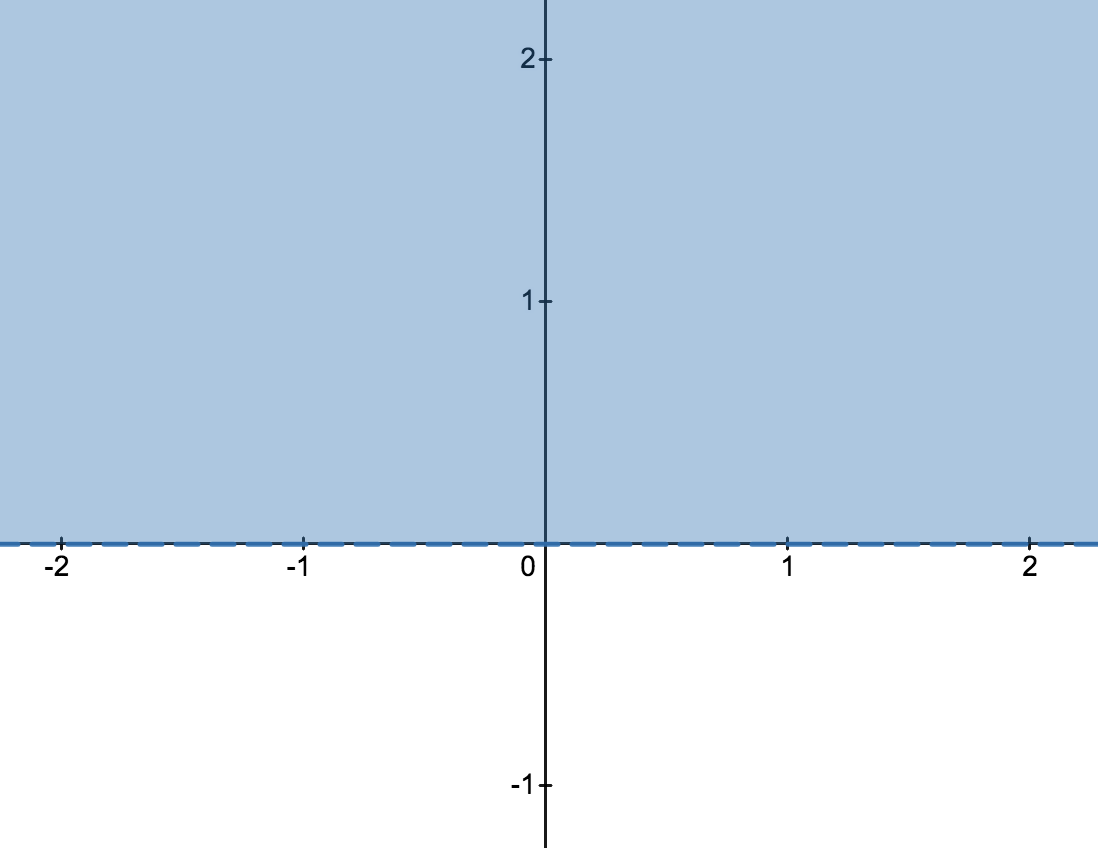
\includegraphics[width=\textwidth]{13a.png}
            \subcaption{$H$.}
            \label{fig:13a}
        \end{subfigure}
        \hfill
        \begin{subfigure}{0.45\textwidth}
            \centering
            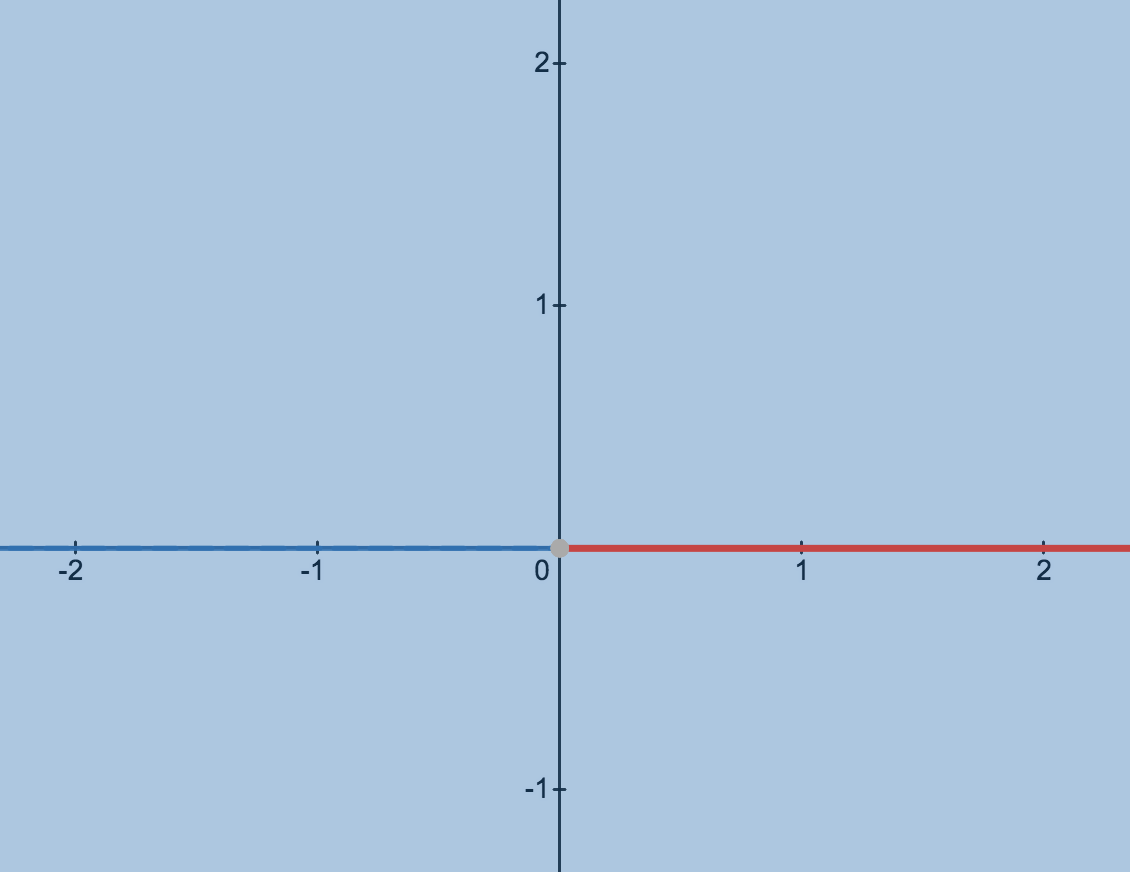
\includegraphics[width=\textwidth]{13b.png}
            \subcaption{$f_1(H)$. The red line consists of all points not included in $f_1(H)$.}
            \label{fig:13b}
        \end{subfigure}
        \caption{Plotted in \cite{Desmos}.}
    \end{figure}
    Next, 
    \[
        \paren{ f_2 \circ f_1 }(H) = -\cx \setminus \setb{ x \in \real \, \middle| \, x \geq 0 } = \cx \setminus \setb{ x \in \real \, \middle| \, x \leq 0 } ,
    \]
    which is in fact the domain $\Omega$ of the principal branch of the logarithm. Then 
    \[
        \paren{ f_3 \circ f_2 \circ f_1 }(H) = 1 + \paren{ \cx \setminus \setb{ x \in \real \, \middle| \, x \leq 0 } } = \cx \setminus \setb{x \in \real \, \middle| \, x \leq 1 } . 
    \]
    \begin{figure}[H]
        \begin{subfigure}{0.45\textwidth}
            \centering
            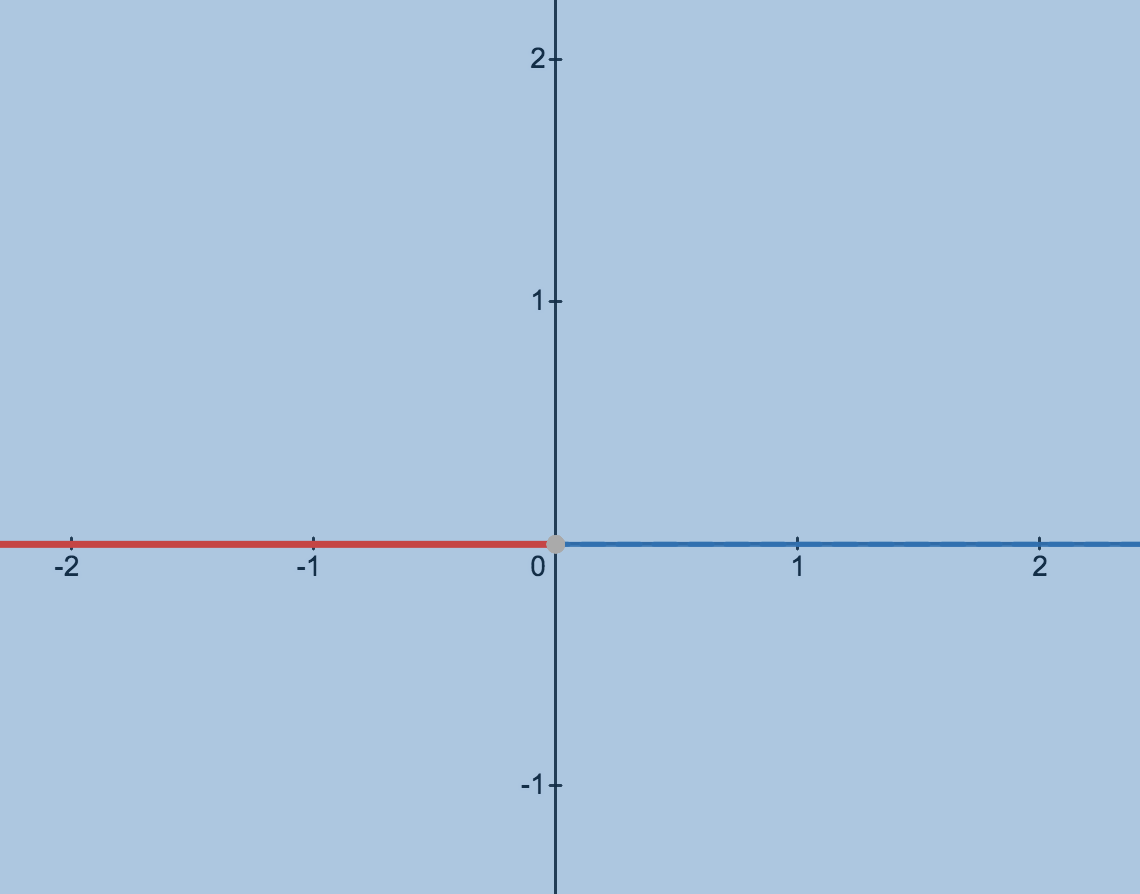
\includegraphics[width=\textwidth]{13c.png}
            \subcaption{$\paren{ f_2 \circ f_1 }(H)$.}
            \label{fig:13c}
        \end{subfigure}
        \hfill
        \begin{subfigure}{0.45\textwidth}
            \centering
            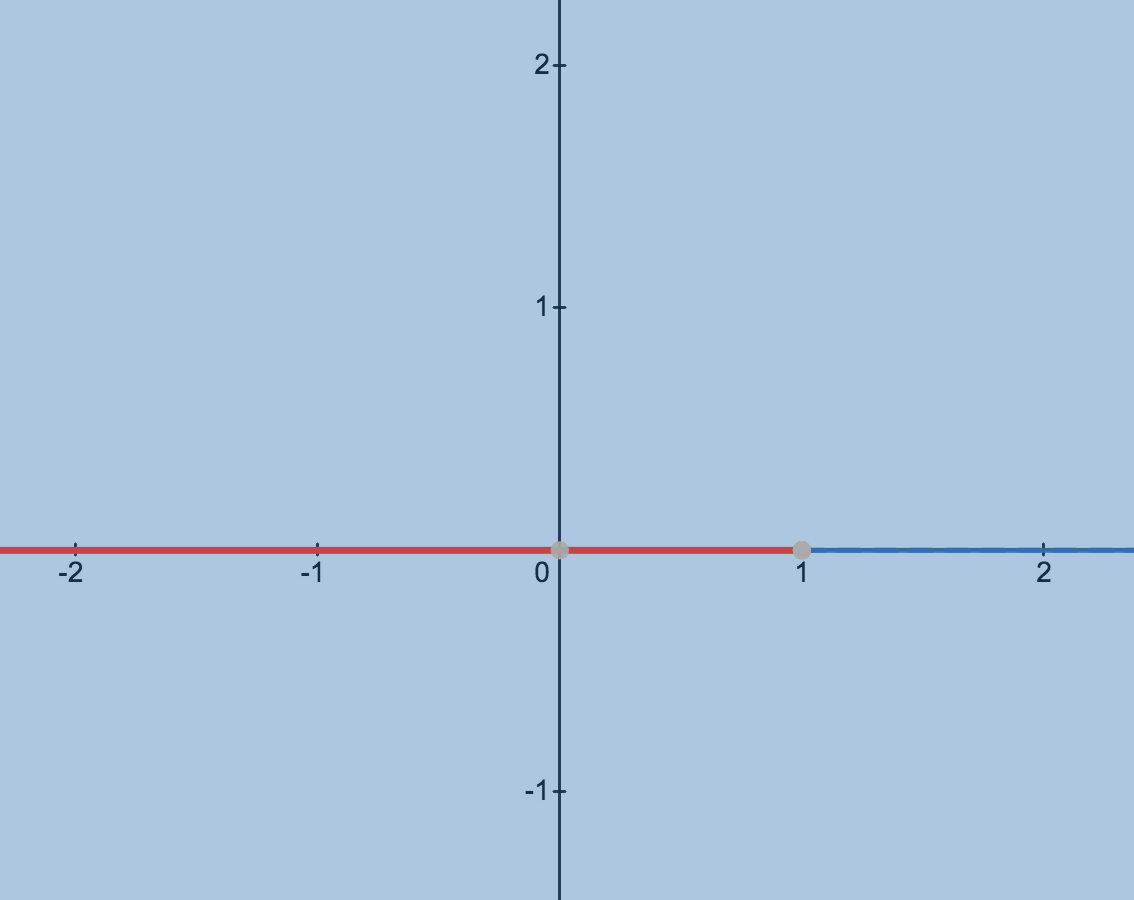
\includegraphics[width=\textwidth]{13d.png}
            \subcaption{$\paren{ f_3 \circ f_2 \circ f_1 }(H)$.}
            \label{fig:13d}
        \end{subfigure}
        \caption{Plotted in \cite{Desmos}.}
    \end{figure}
    Now, recall that 
    \[
        \log(\Omega) = \setb{ w \in \cx \, \middle| \, -\pi < \im(w) < \pi  } = \real \times (-\pi,\pi) . 
    \]
    Furthermore, $\log$ is a bijection between $\Omega$ and $\real \times (-\pi,\pi)$, thus 
    \begin{align*}
        f(H) & = \log \paren{ \paren{ f_3 \circ f_2 \circ f_1 }(H) } = \log \paren{ \cx \setminus \setb{x \in \real \, \middle| \, x \leq 1 } } \\ 
        & = \log \paren{ \Omega \setminus \paren{ (0,1) \times \setb{ 0 } } } = \log(\Omega) \setminus \log \paren{ (0,1) \times \setb{ 0 } } \\ 
        & = \paren{ \real \times (-\pi,\pi) } \setminus \log \paren{ (0,1) \times \setb{ 0 } } . 
    \end{align*}
    Thus it suffices to determine what $\log \paren{ (0,1) \times \setb{ 0 } }$ is. This simplifies to 
    \[
        \ln \paren{ (0,1) } = \paren{ \ln(0),\ln(1) } = (-\infty,0) ,
    \]
    since if $z \in (0,1) \times \setb{ 0 }$, $z$ has zero argument. Then 
    \begin{align*}
        f(H) & = \paren{ \real \times (-\pi,\pi) } \setminus \log \paren{ (0,1) \times \setb{ 0 } } = \paren{ \real \times (-\pi,\pi) } \setminus \paren{ (-\infty,0) \times \setb{ 0 } } \\ 
        & = [0,+\infty) \times (-\pi,\pi) . 
    \end{align*}
    \begin{figure}[H]
        \centering
        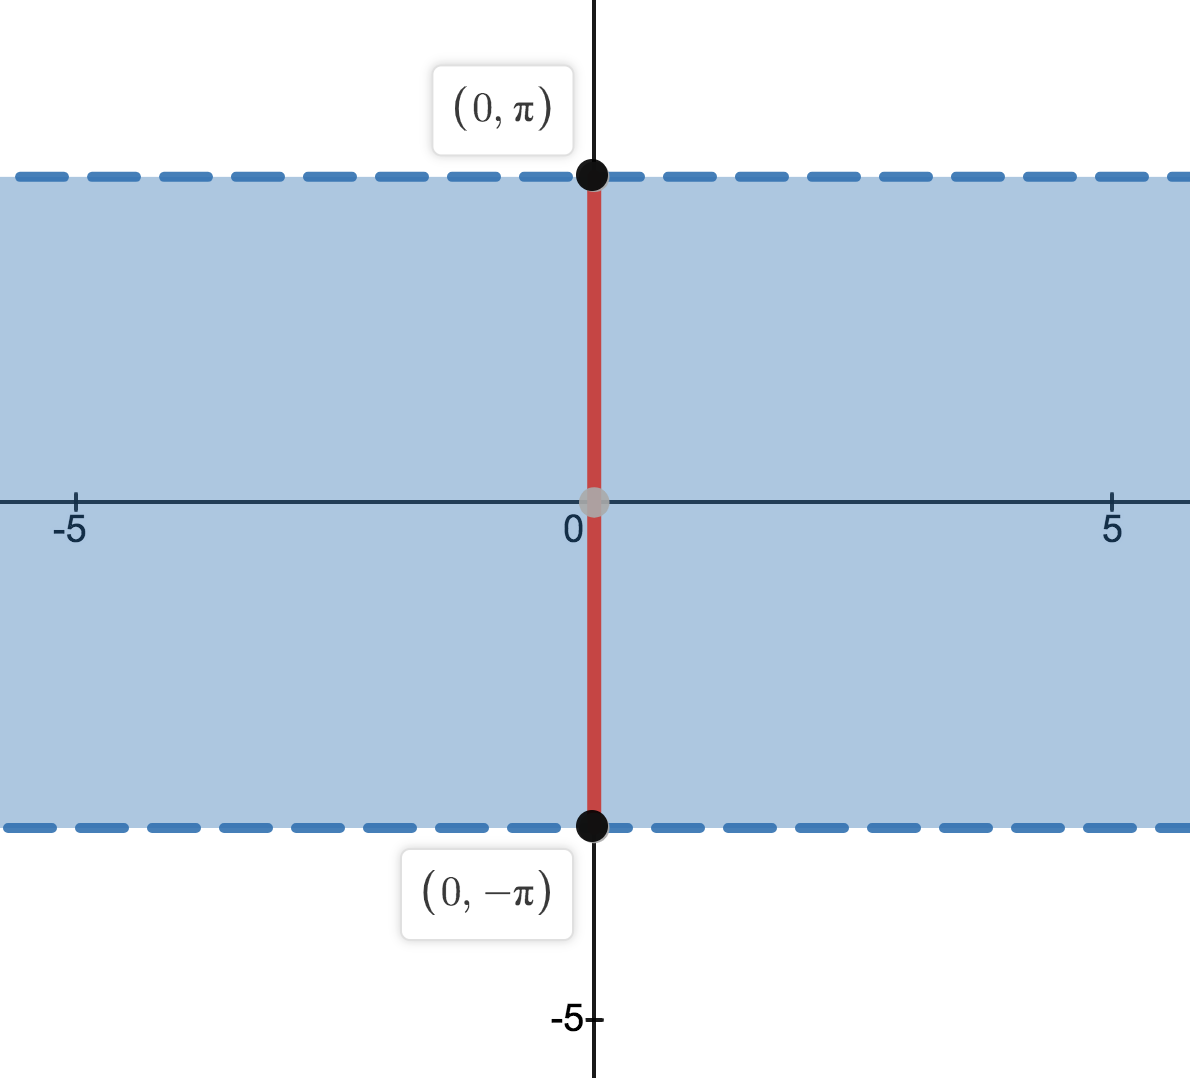
\includegraphics[width = 0.5\textwidth]{13e.png}
        \caption{$f(H)$. The red line consists of all points that are not included in $H$.}
        \label{fig:13e}
    \end{figure}
\end{proof}
\subsection{Problem 3}
Denote by $x$ a real number of modulus less than 1. Develop in a power series in $z$ the infinite product:
\[
    (1 + xz)(1 + x^2z)(1 + x^3z) \dotsc .
\]
\begin{proof}[Answer]
    
\end{proof}
\subsection{Problem 4}
Prove that equation 
\[
    z^3 + wz + w - 0
\]
admits three roots depending analytically on the parameter $w$, in the disk $|w-1| = 1$.
\begin{proof}[Answer]
    
\end{proof}
\subsection{Problem 5 \texorpdfstring{\cite{Melody}}{}}
Let $f(z)$ be a power series in $z$ satisfying the equations $f(z) = z - f(z^2)$. Compute the convergence radius of $f(z)$.
\begin{proof}[Answer]
    Write 
    \[
        f(z) = \sum\limits_{n = 0}^{\infty} a_n (z-a)^n , 
    \]
    for some $a \in \cx$. Without loss of generality, we can take $a = 0$, then the radius of convergence $R$ is given by 
    \[
        \frac{1}{R} = \limsup\limits_{n \to \infty} \sqrt[n]{ \abs{ a_n } } . 
    \]
    Now, substituting the power series into the functional equation gives 
    \[
        \sum\limits_{n = 0}^{\infty} a_n z^n = z - \sum\limits_{n = 0}^{\infty} a_n z^{2n} . 
    \]
    This forces 
    \[
        a_n = 
        \begin{cases}
            1 , & \quad n = 1 , \\ 
            -a_{n/2} , & \quad \text{$n$ even}, \\ 
            0 , & \quad \text{otherwise}.
        \end{cases}
    \]
    Then we can solve the recursion relation $a_{2n} = -a_n$. For $n = 0$, this gives $a_0 = -a_0$, and so $a_0 = 0$. Next, for $n = 1$, we have $a_{2} = -a_1 = -1$, and so in general, $a_{2n} = (-1)^n$ for all $n \geq 1$. Thus $a_n$ is either $0$, $1$, or $-1$, and so 
    \[
        \frac{1}{R} = \limsup\limits_{n \to \infty} \sqrt[n]{ \abs{ a_n } } = 1 . 
    \]
    Thus $R = \boxed{1.}$ Now, we can ever write down an explicit expression for $f$. Using, 
    \[
        f(z) = \sum\limits_{n = 0}^{\infty} a_n z^n = z + \sum\limits_{k = 1}^{\infty} (-1)^k z^{2k} ,
    \]
    then the power series in the RHS is actually the expansion for 
    \[
        -\frac{z^2}{1 + z^2}, 
    \]
    for $\abs{z} < 1$, and so 
    \begin{align*}
        f(z) & = z - \frac{z^2}{1 + z^2} = \frac{z(1+z^2) - z^2}{1 + z^2} \\ 
        & = \frac{z - z^2 + z^3}{1 + z^2} = \frac{ z \paren{ 1 - z + z^2 } }{1 + z^2} ,
    \end{align*}
    for $\abs{z} < 1$. 
\end{proof}

\newpage
\section{Fall 2015 [Completed]}
Answer three complete questions in each of the two sections Real Analysis, Complex Analysis. 

\subsection{Problem 1}
Suppose the power series $\sum_n a_n (z - a)^n$ converges for $z = z_1$ some point in the complex plane. Show the series converges absolutely for all $z$ with $\abs{z - a} < \abs{z_1 - a}$, i.e. in a disk of radius $\abs{z_1 - a}$ centered at $a$.
\begin{proof}[Answer]
    Let 
    \[
        \frac{1}{R} \coloneqq \limsup\limits_{n \to \infty} \sqrt[n]{ \abs{ a_n } }
    \]
    be the radius of convergence of the power series
    \[
        \sum\limits_{n = 0}^{\infty} a_n \paren{ z - a_n }^n . 
    \]
    Then the series converges absolutely for all $\abs{z - a} < R$ and diverges for all $\abs{z - a} > R$. Since the power series converges at $z = z_1$, we must have $\abs{z_1 - a} < R$, and so the power series will converge absolutely for $\abs{z - a} < \abs{z_1 - a} < R$. 
\end{proof}

\subsection{Problem 2}
Compute the improper integral 
\[
    \i{-\infty}{\infty}{\frac{1}{1+x^2}}{x}
\]
being sure to justify all the estimates you make. 
\begin{proof}[Answer]
    See Fall 1992, Problem 5. 
\end{proof}

\subsection{Problem 3}
For $\re(s) > 0$ we define the Gamma function by 
\[
    \Gamma(s) = \i{0}{\infty}{\exp(-x)x^{s-1}}{x} . 
\]
Assuming the integral converges absolutely (which is not hard to show), prove that the function $\Gamma(s)$ is a holomorphic function in the region $\Omega : \re(s) > 0$. Hint: Morera's Theorem. 
\begin{proof}[Answer]
    It suffices to show that 
    \[
        \i{C}{}{\Gamma(s)}{s} = 0
    \]
    for every circle contained in $\re(s) > 0$. Note that 
    \[
        \i{C}{}{\Gamma(s)}{s} = \i{C}{}{ \i{0}{\infty}{x^{s-1}e^{-x}}{x} }{s} . 
    \]
    If we can justify swapping the integrals, then we can write
    \begin{equation}\label{swap}
        \i{C}{}{\Gamma(s)}{s} = \i{C}{}{ \i{0}{\infty}{x^{s-1}e^{-x}}{x} }{s} = \i{0}{\infty}{ \i{C}{}{x^{s-1}e^{-x}}{s} }{x} . 
    \end{equation}
    Then if we can show that the function $f(s) \coloneqq x^{s-1} e^{-x}$ is analytic on 
    \[
        \Omega \coloneqq \setb{ s \in \cx \, \middle| \, \re(s) > 0 } ,  
    \]
    then by Cauchy's Theorem 
    \[
        \i{C}{}{\Gamma(s)}{s} = \i{0}{\infty}{ \i{C}{}{x^{s-1}e^{-x}}{s} }{x} = \i{0}{\infty}{ 0 }{x} = 0. \, \checkmark 
    \]
    Thus by Morera's Theorem, $\Gamma$ is analytic on $\Omega$. 
    \begin{claim}
        $f(s) \coloneqq x^{s-1} e^{-x}$ is analytic on $\Omega$, for any $x \in (0,+\infty)$. 
    \end{claim}
    \begin{proof}
        This is actually the more pressing claim to take care of, since raising a complex number to a non-integer power is always a complicated thing. Recall that for any $z \in \cx^{\times}$, $\alpha \in \cx$, by $z^{\alpha}$ we really mean 
        \[
            z^{\alpha} \coloneqq e^{\alpha \log(z)}
        \]
        for some appropriate branch of the logarithm. Since $\Omega$ excludes the non-negative real numbers, we can use the principal branch of the logarithm 
        \[
            \Log \paren{ re^{i\theta} } = \ln(r) + i\theta
        \]
        for $r > 0$, $-\pi < \theta < \pi$. Since $x \in (0,+\infty)$, we simply have 
        \[
            f(s) = x^{s-1} e^{-x} = e^{(s-1) \Log(x)} e^{-x} = \exp \sqbrack{ \ln(x) (s - 1) - x } , 
        \]
        and so $f$ analytic on $\Omega$ for any $x \in (0,+\infty)$, since it is just an exponential function!
    \end{proof}
    \begin{claim}
        Swapping the integrals in \eqref{swap} is justified. 
    \end{claim}
    \begin{proof}
        Parametrize $C$ as 
        \[
            C = \setb{ a + re^{i\theta} \, \middle| \, -\pi < \theta \leq \pi }
        \]
        for some $a \in \Omega$, $r > 0$ such that $C$ lies entirely in $\Omega$. Then 
        \begin{align*}
            \i{C}{}{\Gamma(s)}{s} & = \i{-\pi}{\pi}{\Gamma \paren{ a + re^{i\theta} } i re^{i\theta}}{\theta} = ir \i{-\pi}{\pi}{ \i{0}{\infty}{ x^{ \paren{ a + re^{i\theta} } - 1} e^{-x} }{x} }{\theta} \\ 
            & = ir \i{-\pi}{\pi}{ \i{0}{\infty}{ \underbrace{ e^{ \paren{ a + re^{i\theta}  - 1} \Log(x) } e^{-x} }_{ \eqqcolon g(x,\theta) } }{x} }{\theta} . 
        \end{align*}
        Then taking $g : (0,+\infty) \times (-\pi,\pi] \to \cx$, $g$ is continuous (in fact smooth!), and it is measurable. Then by Fubini's Theorem, 
        \begin{align*}
            \i{C}{}{\Gamma(s)}{s} & = ir \i{-\pi}{\pi}{ \i{0}{\infty}{ e^{ \paren{ a + re^{i\theta}  - 1} \Log(x) } e^{-x} }{x} }{\theta} = ir \i{0}{\infty}{ \i{-\pi}{\pi}{ e^{ \paren{ a + re^{i\theta}  - 1} \Log(x) } e^{-x} }{\theta} }{x} \\ 
            & = \i{0}{\infty}{ \i{C}{}{e^{(s-1)\Log(x)}e^{-x}}{s} }{x} . \, \checkmark 
        \end{align*}
    \end{proof}
    Lastly, it is in fact not hard to show that $\Gamma(s)$ converges absolutely: 
    \begin{align*}
        \abs{ \Gamma(s) } & = \abs{ \i{0}{\infty}{x^{s-1}e^{-x}}{x} } \leq \i{0}{\infty}{\abs{ x^{s-1} e^{-x} }}{x} \\ 
        & = \i{0}{\infty}{ \abs{ x^{s-1} } \abs{ e^{-x} } }{x} = \i{0}{\infty}{ \abs{ e^{(s-1)\ln(x)} } e^{-x} }{x} \\ 
        & = \i{0}{\infty}{ e^{ \re \sqbrack{ (s - 1) \ln(x) } } e^{-x} }{x} = \i{0}{\infty}{ e^{ \re(s-1) \ln(x)  } e^{-x} }{x} \\ 
        & = \i{0}{\infty}{ x^{\re(s-1)} e^{-x} }{x} = \i{0}{\infty}{ x^{\re(s)-1} e^{-x} }{x} . 
    \end{align*}
    Then it suffices to show that $\Gamma(s)$ converges absolutely for $s > 0$. Writing
    \[
        \i{0}{\infty}{x^{s-1}e^{-x}}{x} = \i{0}{1}{x^{s-1}e^{-x}}{x} + \i{1}{\infty}{x^{s-1}e^{-x}}{x} , 
    \]
    then the second integral converges since $x^{s-1}$ is bounded near $x = 1$, while the exponential term dominates the long term behavior. For the first integral, since $e^{-x} \leq 1$ for $0 \leq x \leq 1$, we have 
    \[
        \i{0}{1}{x^{s-1}e^{-x}}{x} \leq \i{0}{1}{x^{s-1}}{x} = \left. \frac{x^s}{s} \right|_{x = 0}^{x = 1} = \frac{1}{s} < +\infty 
    \]
    for all $s > 0$. 
\end{proof}

\subsection{Problem 4}
Suppose $\setb{ s_n(z) }$ is a sequence of continuous functions, uniformly convergent to $f(z)$ in $\Omega$, and $\Gamma$ is a rectifiable curve in $\Omega$. Show that the sequence 
\[
    \setb{ \i{\Gamma}{}{s_n(z)}{z} } \quad \text{converges to} \quad \i{\Gamma}{}{f(z)}{z} . 
\]
\begin{proof}[Answer]
    Consider 
    \[
        \abs{ \i{\Gamma}{}{s_n(z)}{z} - \i{\Gamma}{}{f(z)}{z} } = \abs{ \i{\Gamma}{}{ \sqbrack{ s_n(z) - f(z) } }{z} } \leq \int_{\Gamma} \abs{ s_n(z) - f(z) } \, \abs{ \rd z } . 
    \]
    Since $s_n$ converges uniformly to $f$ in $\Omega$, for given $\eps > 0$ there exists $N \in \z^+$ such that 
    \[
        \abs{ s_n(z) - f(z) } < \frac{\eps}{V(\Gamma)} 
    \]
    for all $z \in \Omega$, $n > N$. Thus 
    \begin{align*}
        \abs{ \i{\Gamma}{}{s_n(z)}{z} - \i{\Gamma}{}{f(z)}{z} } & \leq \int_{\Gamma} \abs{ s_n(z) - f(z) } \, \abs{ \rd z } < \int_{\Gamma} \frac{\eps}{V(\Gamma)} \, \abs{ \rd z } \\ 
        & = \frac{\eps}{V(\Gamma)} \int_{\Gamma} \, \abs{ \rd z } = \frac{\eps}{V(\Gamma)} \cdot V(\Gamma) \\ 
        & = \eps ,
    \end{align*}
    for all $n > N$. Thus 
    \[
        \i{\Gamma}{}{s_n(z)}{z} \to \i{\Gamma}{}{f(z)}{z}
    \]
    as $n \to \infty$. 
\end{proof}

\subsection{Problem 5}
Suppose $f(z)$ is entire and not constant. Show that the image of $f$ is dense in $\cx$.
\begin{proof}[Answer]
    By way of contradiction, suppose that $f(\cx)$ is not dense in $\cx$. Then there exists $w_0 \in \cx$ and $r > 0$ such that $\abs{ w_0 - f(z) } \geq r$ for all $z \in \cx$. In particular, $w_0 - f(z)$ never vanishes on $\cx$. Then 
    \[
        g(z) \coloneqq \frac{1}{w_0 - f(z)}
    \]
    is an entire function and is also bounded, since 
    \[
        \abs{ g(z) } = \abs{ \frac{1}{w_0 - f(z)} } = \frac{1}{\abs{ \frac{1}{w_0 - f(z)} }} \leq \frac{1}{r} . 
    \]
    By Liouville's Theorem, $g$ must be constant, say $g(z) \equiv \alpha$ for some $\alpha \in \cx$. Since $g$ never vanishes, $\alpha \neq 0$ and so $\frac{1}{\alpha}$ exists. Then 
    \begin{align*}
        \alpha & \equiv g(z) = \frac{1}{w_0 - f(z)} , \\ 
        \Rightarrow \frac{1}{\alpha} & \equiv w_0 - f(z) , \\ 
        \Rightarrow f(z) & \equiv \frac{1}{\alpha} - w_0 , 
    \end{align*}
    and so $f$ is constant, a contradiction. Therefore the image of $f$ must be dense in $\cx$. 
\end{proof}

\newpage
\section{Spring 2016 [Answered]}
Answer three complete sections in each of the two sections Real Analysis, Complex Analysis. Each problem is worth 10 points. You must fully justify all of your answers in order to get full credit. 

\subsection{Problem 1 \texorpdfstring{\cite{Israel}}{}}
Compute $\int_0^{\pi} e^{\cos t} \, dt$. 
\begin{proof}[Answer]
    First, write 
    \[
        I \coloneqq \i{0}{\pi}{e^{\cos(t)}}{t} = \frac{1}{2} \i{0}{2\pi}{ e^{ \cos \paren{ \frac{\theta}{2} } } }{\theta} . 
    \]
    Note that for $\abs{z} = 1$, $\inv{z} = \bar{z}$, and so 
    \[
        \re(z) = \frac{z + \bar{z}}{2} = \frac{z + \frac{1}{z}}{2} . 
    \]
    Let 
    \[
        f(z) \coloneqq \frac{ e^{ \frac{z + \frac{1}{z}}{2} } }{z} , 
    \]
    and let $\gamma : [0,2\pi] \to \cx$, $\gamma(\theta) \coloneqq e^{i\frac{\theta}{2}}$. Then 
    \[
        \i{\gamma}{}{f(z)}{z} = \i{0}{2\pi}{ f \paren{ e^{i\frac{\theta}{2}} } \frac{i}{2} e^{i\frac{\theta}{2}} }{\theta} = \frac{i}{2} \i{0}{2\pi}{ \frac{ e^{\cos \paren{ \frac{\theta}{2} } } }{e^{i\frac{\theta}{2}}} e^{i\frac{\theta}{2}} }{\theta} = i I. 
    \]
    On the other hand, by Residue Theorem, 
    \[
        \i{\gamma}{}{f(z)}{z} = 2\pi i n(\gamma;0) \Res(f;0) = 2\pi i a_{-1} , 
    \]
    where $a_{-1}$ is the coefficient of $\frac{1}{z}$ from a Laurent expansion of $f$ in an annulus centered at the origin. Thus $I = 2\pi a_{-1}$. Now, on $\cx^{\times}$ we have the Laurent expansion 
    \begin{align*}
        f(z) & = \frac{ e^{ \frac{z + \frac{1}{z}}{2} } }{z} = \frac{e^{\frac{z}{2}}}{z} e^{\frac{1}{2z}} \\ 
        & = \frac{e^{\frac{z}{2}}}{z} \sum\limits_{n = 0}^{\infty} \frac{1}{2^n z^n n!} = e^{\frac{z}{2}} \sum\limits_{n = 0}^{\infty} \frac{z^{-n-1}}{2^n n!} \\ 
        & = \paren{ \sum\limits_{n = 0}^{\infty} \frac{z^n}{2^n n!} } \paren{ \sum\limits_{n = 0}^{\infty} \frac{z^{-n-1}}{2^n n!} } . 
    \end{align*}
    Now, the residue of the above series comes from multiplying the coefficients for $z^n$ and $z^{-n-1}$ together and summing them up from $n = 1$ to $\infty$. Thus 
    \[
        I = 2\pi \Res(f;0) = 2\pi \sum\limits_{n = 1}^{\infty} \paren{ \frac{1}{2^n n!} }^2 \approx 1.6714. 
    \]
\end{proof}

\subsection{Problem 2}
Prove that if $P(z)$ is a polynomial with at least two distinct roots, then no component of the planar curve given by the equation $|P(z)| = 1$ can be a circle. 
\begin{proof}[Answer]
    UNANSWERED 
\end{proof}

\subsection{Problem 3 \texorpdfstring{\cite{Nguyen}}{}}
Find an explicit analytic function in $\mathbf{C} \setminus [-1,1]$ which is bounded and non-constant. 
\begin{proof}[Answer]
    First, note that $\Omega \coloneqq \cx \setminus [-1,1]$ is an open and connected subset of $\cx^{\times}$ that does not contain $S^1$. Thus a branch of the logarithm exists and is analytic on $\Omega$. Let $f : \Omega \to \cx$, 
    \[
        f(z) \coloneqq \frac{w}{1 + w} , 
    \]
    where 
    \[
        w \coloneqq \sqrt{ \frac{z-1}{z+1} } . 
    \]
    Here we take 
    \[
        \abs{z} = e^{\frac{1}{2}\log(z)} . 
    \]
    We show that $f$ is analytic. Firstly, note that $w$ is defined and does not vanish on $\Omega$. Next, we need to show that the denominator of $f$ does not vanish. This happens if and only if 
    \begin{align*}
        -1 & = \sqrt{ \frac{z - 1}{z + 1} } , \\ 
        \Rightarrow 1 & = \frac{z - 1}{z + 1} , \\ 
        \Rightarrow z + 1 & = z - 1 , \\ 
        \Rightarrow 1 & = -1 . \, \Rightarrow \Leftarrow 
    \end{align*}
    Thus $f$ is analytic on $\Omega$. Next, we show that $f$ is bounded. UNFINISHED
\end{proof}

\subsection{Problem 4 \texorpdfstring{\cite{Nguyen}}{}}
Let $f(z)$ be an analytic function defined in a disk $\abs{z} < r$. Show that the functional equation $f(2z) = f(z) f'(z)$ satisfied on $|z| < r/2$ implies that $f(z)$ is an entire function. 
\begin{proof}[Answer]
    Note that if $f(2z) = f(z) f'(z)$ holds for $\abs{z} < \frac{r}{2}$, then 
    \[
        f(z) = f \paren{ \frac{z}{2} } f' \paren{ \frac{z}{2} }
    \]
    for $z \in r$. But then the RHS holds for 
    \[
        \abs{ \frac{z}{2} } < r \Rightarrow \abs{z} < 2r ,
    \]  
    and so $f$ is analytic on $\abs{z} < 2r$. Repeat this process to obtain that $f$ is analytic on $\abs{z} < 2^n r$ for all $n \in \n$, and so $f$ is analytic on all of $\cx$, that is, $f$ is entire. 
\end{proof}

\subsection{Problem 5 \texorpdfstring{\cite{Conway}}{}}
State and prove Rouch\'e's theorem. 
\begin{proof}[Answer]
    Let $f$ and $g$ are meromorphic in a neighborhood of the bounded domain $D \subset \cx$. Let $Z_f$, $Z_g$, $P_f$, $P_g$ be the number of zeros and poles of $f$ and $g$, respectively, in $D$ counted with multiplicity. If   
    \[
        \abs{ f(z) + g(z) } < \abs{ f(z) } + \abs{ g(z) }
    \]
    for all $z \in \partial D$, then 
    \[
        Z_f - P_f = Z_g - P_g . 
    \]
    First, note that $\abs{ f(z) + g(z) } < \abs{ f(z) } + \abs{ g(z) }$ for all $z \in \partial D$ implies that $f$ and $g$ do not vanish on $\partial D$, otherwise we have, without loss of generality, a zero $z_0$ for $f$ on $\partial D$, and so 
    \[
        \abs{ f \paren{ z_0 } + g \paren{ z_0 } } = \abs{ g \paren{ z_0 } } < \abs{ f \paren{ z_0 } } + \abs{ g \paren{ z_0 } } = \abs{ g \paren{ z_0 } } , 
    \]
    a contradiction. Then by hypothesis, 
    \begin{align*}
        \abs{ f(z) + g(z) } & < \abs{ f(z) } + \abs{ g(z) } \\ 
        \Rightarrow \frac{ \abs{ f(z) + g(z) } }{ \abs{ g(z) } } & < \frac{ \abs{ f(z) } + \abs{ g(z) } }{ \abs{ g(z) } } , \\ 
        \Rightarrow \abs{ \frac{f(z) + g(z)}{g(z)} } & = \abs{ \frac{f(z)}{g(z)} + 1 } < \abs{ \frac{f(z)}{g(z)} } + \abs{ \frac{g(z)}{g(z)} } = \abs{ \frac{f(z)}{g(z)} } + 1 
    \end{align*}
    for all $z \in \partial D$. Set 
    \[
        h(z) \coloneqq \frac{f(z)}{g(z)} , 
    \]
    then if $h(z) \in (0,+\infty)$, we have 
    \begin{align*}
        \abs{ \frac{f(z)}{g(z)} + 1 } & < \abs{ \frac{f(z)}{g(z)} } + 1 , \\ 
        \Rightarrow h(z) + 1 & < h(z) + 1 , 
    \end{align*}
    a contradiction. Thus $h \paren{ \partial D } \subset \Omega \coloneqq \cx \setminus [0,+\infty)$. Then a branch of the logarithm exists on $\Omega$, thus 
    \[
        \log \sqbrack{ \frac{f(z)}{g(z)} }
    \]
    is a well-defined primitive for 
    \[
        \sqbrack{ \frac{f(z)}{g(z)} }' \sqbrack{ \frac{f(z)}{g(z)} }^{-1} = \frac{f'(z)g(z) - f(z)g'(z)}{g(z)^2} \cdot \frac{g(z)}{f(z)} = \frac{f'(z)}{f(z)} - \frac{g'(z)}{g(z)} . 
    \]
    Thus 
    \begin{align*}
        0 & = \frac{1}{2\pi i} \i{\partial D}{}{ \sqbrack{ \frac{f(z)}{g(z)} }' \sqbrack{ \frac{f(z)}{g(z)} }^{-1} }{z} = \i{\partial D}{}{ \sqbrack{ \frac{f'(z)}{f(z)} - \frac{g'(z)}{g(z)} } }{z} \\ 
        & = \i{\partial D}{}{ \frac{f'(z)}{f(z)} }{z} - \i{\partial D}{}{ \frac{g'(z)}{g(z)} }{z} = \paren{ Z_f - P_f } - \paren{ Z_g - P_g } , 
    \end{align*}
    by the Argument Principle. 
\end{proof}

\section{Fall 2016 [Answered]}
Solve 3 of the 5 problems in both Parts 1 and 2. Each problem is worth 10 points. This exam will test your knowledge in analysis as well as the clarity of your mathematical writing, so be sure to show all your work and justify all your steps. You must pass \textbf{both} parts in order to pass the exam. 

\subsection{Problem 1}
Prove that for any $n \in N$, $n \geq 2$
\[
    \int_0^{\infty} \frac{1}{1 + x^n} dx = \frac{\pi}{n \sin(\pi/n)} . 
\]
Suggestion: Consider $\int_{C_R} \frac{1}{1 + z^n}dz$ where $C_R$, $R > 1$, is the positively oriented contour given by 
\[
    \setb{x : 0 \leq x \leq R} \cup \setb{ Re^{i\theta} : 0 \leq \theta \leq 2\pi / n } \cup \setb{ re^{i2\pi/n} : R \geq r \geq 0  }. 
\]
\begin{proof}[Answer]
    See Spring 1994, Problem 7. 
\end{proof}

\subsection{Problem 2}
Let $f(z)$ be an analytic function in the unit disk 
\[
    D = \setb{ z \in \cx : \abs{z} < 1 } . 
\]
Suppose that 
\[
    f(0) = 0 \text{ and } \abs{ f(z) } \leq \text{ for } z \in D . 
\]
Prove Schwarz' Lemma, namely: 
\begin{enumerate}[(a)]
    \item $\abs{ f(z) } \leq \abs{ z }$ for $z \in D$, 
    \item $\abs{ f'(0) } \leq 1$, and 
    \item if there exists $z_0 \in D$ such that $z_0 \neq 0$ and $\abs{ f \paren{ z_0 } } = \abs{ z_0 }$, then 
    \[
        f(z) = e^{i\theta} z , \quad \text{for some } \theta \in \real . 
    \]
    Suggestion: Apply the maximum modulus theorem to the function $f(z) / z$.
\end{enumerate}
\begin{proof}[Answer]
    See Spring 2014, Problem 2. 
\end{proof}

\subsection{Problem 3}
Suppose that $f(z)$ is analytic on $\cx$ and that there exists a constants $A > 0$ and $B > 0$ such that $\abs{ f(z) } \leq A \abs{z}^{1/2} + B$ for all $z \in \cx$. What can you say about $f(z)$?
\begin{proof}[Answer]
    
\end{proof}

\subsection{Problem 4 \texorpdfstring{\cite{Melody}}{}}
Let $f(z)$ be analytic function on $\cx$ such that at each point of $\cx$ some derivative of $f(z)$ is zero. Prove that $f(z)$ is a polynomial. 
\begin{proof}[Answer]
    Recall that if $f , g$ are analytic functions on a domain $\Omega \subseteq \cx$ that are equal on a set with an accumulation point, then $f = g$ on $\Omega$. We show that $f$ is equal to a polynomial on a set with an accumulation point, and so $f$ must be a polynomial. 
    
    Let
    \[
        E_n \coloneqq \setb{ z \in \cx \, \middle| \, f^{(n)}(z) = 0 } = \inv{ \paren{ f^{(n)} } } \paren{ \setb{ 0 } } , 
    \]
    for each $n \in \n$. Then by hypothesis, $E_n \neq \varnothing$ for all $n \in \n$, and 
    \[
        \bigcup\limits_{n = 0}^{\infty} E_n = \cx . 
    \]
    Since $\cx$ is uncountable, there exists $N \in \z^+$ such that $E_N$ is uncountable. Then $E_N$ must have an accumulation point (since $\cx$ is Lindel\"of!), and so we show that $f$ is equal to a polynomial on $E_N$. 
    
    Write 
    \[
        f(z) = \sum\limits_{n = 0}^{\infty} a_n z^n ,
    \]
    where 
    \[
        a_n = \frac{f^{(n)}(0)}{n!} . 
    \]
    Then for all $z \in E_N$, $f^{(N)}(z) = 0$, and so 
    \[
        f(z) = \sum\limits_{n = 0}^{\infty} a_n z^n = \sum\limits_{n = 0}^{N-1} a_n z^n ,  
    \]
    and so $f$ is equal to a polynomial on $E_N$. 
\end{proof}

\subsection{Problem 5}
Define 
\[
    g(z) = \frac{1}{(z-1)(z-2)} . 
\]
Find the Laurent series expansion of $g(z)$ about $z = 0$ in the domain 
\[
    \setb{ 1 < \abs{z} < 2 } . 
\]
\begin{proof}[Answer]
    
\end{proof}

\newpage
\section{Spring 2017 [Answered]}
Solve 3 out of the 5 problems in both Part 1 and Part 2. 

\subsection{Problem 1}
Let $\bar{\cdot}$ denote complex conjugation. Prove that if $f(z)$ is an analytic function, then $\bar{f}(\bar{z})$ is also an analytic function. 
\begin{proof}[Answer]
    Writing 
    \[
        f(z) = f(x + iy) = u(x,y) + i v(x,y) , 
    \]
    then as $f$ is analytic, it satisfies the Cauchy-Riemann equations
    \[
        u_x(x,y) = v_y(x,y) , \qquad u_y(x,y) = - v_x(x,y) . 
    \]
    Write 
    \[
        \bar{f} \paren{ \bar{z} } = \overline{ f(x - iy) } = u(x,-y) - i v(x,-y) = U(x,y) + i V(x,y) , 
    \]
    where $U(x,y) \coloneqq u(x,-y)$, $V(x,y) \coloneqq -v(x,-y)$. Then it suffices to show that $U$ and $V$ also satisfy the Cauchy-Riemann equations: 
    \begin{align*}
        U_x(x,y) & = u_x(x,-y) \\ 
        & = v_y(x,-y) && \text{since $u$ and $v$ satisfy cauchy-Riemann} \\ 
        & = V_y(x,y) , \, \checkmark \\ 
        U_y(x,y) & = \frac{\partial}{\partial y} \sqbrack{ u(x,-y) } \\ 
        & = - u_y(x,-y) && \text{by Chain Rule} \\ 
        & = v_x(x,-y) && \text{since $u$ and $v$ satisfy cauchy-Riemann} \\ 
        & = -V_x(x,y) . \, \checkmark 
    \end{align*}
    Therefore $\bar{f} \paren{ \bar{z} }$ is analytic. 
\end{proof}

\subsection{Problem 2}
Suppose that $f(z)$ is analytic and satisfies the condition $\abs{f(z) - 1} < 1$ in a region $\Omega$. Prove that $\re f(z) > 0$ throughout $\Omega$.
\begin{proof}[Answer]
    
\end{proof}

\subsection{Problem 3}
Compute 
\[
    \int_{\abs{z} = 2} \frac{dz}{z^2 + 1}
\]
by decomposing the integrand into partial fractions. 

\begin{proof}[Answer]
    Since 
    \[
        f(z) \coloneqq \frac{1}{z^2 + 1} = \frac{1}{(z - i)(z+ i)} , 
    \]
    the circle $\abs{z} = 2$ encircles all of the poles of $f$. Thus 
    \[
        \i{\abs{z} = 2}{}{f(z)}{z} = 2\pi i \sqbrack{ \Res(f;i) + \Res(f;-i) } = \boxed{0.}
    \]
\end{proof}

\subsection{Problem 4}
Use a conformal map to map the region enclosed between the curves $\abs{z} = 1$ and $\abs{z - \frac{1}{2}} = \frac{1}{2}$ onto the upper half plane. Draw the mapped region. 
\begin{proof}[Answer]
    
\end{proof}

\subsection{Problem 5 \texorpdfstring{\cite{Joel}}{}}
How many roots does the question 
\[
    z^7 + 2z^5 + 6z^3 - z + 1 = 0
\]
have in the disk $\abs{z} < 1$? (Hint: The function to compare with in Rouch\'e's theorem is not always the highest power of $z$.)
\begin{proof}[Answer]
    Let 
    \begin{align*}
        f(z) \coloneqq z^7 + 2z^5 + 6z^3 - z + 1 , \\ 
        g(z) \coloneqq 2z^5 + 6z^3 = 2z^3 \paren{ z^2 + 3 } = 2z^3 \paren{ z - i \sqrt{3} } \paren{ z + i \sqrt{3} } . 
    \end{align*}
    Since $\sqrt{3} > 1$, $g$ has 3 roots counted with multiplicity in $\abs{z} < 1$. Then for $\abs{z} = 1$, 
    \begin{align*}
        \abs{ f(z) - g(z) } & = \abs{ z^7 + 2z^5 + 6z^3 - z + 1 - 2z^5 - 6z^3 } \\ 
        & = \abs{ z^7 - z + 1 } \leq \abs{ z^7 } + \abs{ -z } + \abs{1} \\ 
        & = \abs{z}^7 + \abs{z} + 1 \leq 1 + 1 + 1 \\ 
        & = 3 , 
    \end{align*}
    while 
    \begin{align*}
        \abs{ f(z) } & \geq \abs{ 6z^3 } - \abs{ z^7 + 2z^5 - z + 1 } \geq \abs{ 6z^3 } - \abs{ z^7 } - \abs{ 2z^5 } - \abs{ -z } - \abs{1} \\ 
        & = 6 \abs{z}^3 - \abs{z}^7 - 2 \abs{z}^5 - \abs{z} - 1 \geq 6 - 1 - 2 - 1 - 1 \\ 
        & = 1 , \\ 
        \abs{ g(z) } & \geq \abs{ 6z^3 } - \abs{ 2z^5 } = 6 \abs{z}^3 - 2 \abs{z}^5 \\ 
        & = 6 - 2 = 4 .
    \end{align*}
    Thus 
    \[
        \abs{ f(z) - g(z) } \leq 3 \leq 5 = 1 + 4 \leq \abs{f(z)} + \abs{g(z)} ,
    \]
    and so by Rouch\'e's Theorem, $f$ have the same number of zeros counted with multiplicity in $\abs{z} = 1$ as $g$ does, namely $\boxed{3.}$
\end{proof}

\newpage 
\section{Fall 2017}
Answer three complete questions in each of the two sections Real Analysis, Complex Analysis. Remember to justify all assertions. 

\subsection{Problem 1}
Is there an analytic function $f$ in $\cx \setminus \setb{ 0 }$ such that $\abs{ f(z) } \geq \frac{1}{\sqrt{\abs{z}}}$. 
\begin{proof}[Answer]
    
\end{proof}

\subsection{Problem 2}
Compute the improper integral 
\[
    \i{-\infty}{\infty}{ \frac{\sin^3(x)}{x^3} }{x} . 
\]
Hint: Expand $\sin^3(x)$ and simplify first. 
\begin{proof}[Answer]
    
\end{proof}

\subsection{Problem 3}
In what annuli centered at $0$ can the function $3/[z(z+3)]$ be expanded in a Laurent series. Find that series in each annulus and (of course) prove that it converges to the function. 
\begin{proof}[Answer]
    
\end{proof}

\subsection{Problem 4}
Suppose that $g$ is analytic in the open unit disk except at $0$ and $\Re(g) \geq 0$ there. Prove that the singularity at $0$ is removable. \ita{Hint}: can the origin be an essential singularity?
\begin{proof}[Answer]
    
\end{proof}

\subsection{Problem 5}
Suppose that $f$ is analytic on the open unit disk $D$ and $f(0) = 0$. Prove or disprove that the series $\sum_1^{\infty} f (z^n)$ converges uniformly on compact subsets of $D$.
\begin{proof}[Answer]
    
\end{proof}

\newpage 
\section{Spring 2018}

\newpage 
\section{Fall 2018}

\newpage 
\section{Spring 2019 [Answered]}
\ita{Do 4 of out of the following 5 problems.}
\subsection{Problem 1}
Find the radius of convergence of the power series 
\[
    \sum\limits_{n = 0}^{\infty} \paren{ \cos n } z^n . 
\]
\begin{proof}[Answer]
    Recall that $\abs{ \cos(n) } \leq 1$ for all $n \in \z^+$. Then for any $\delta > 0$ there exists $n \in \z^+$ large enough such that 
    \[
        n - 2\pi \fl{ \frac{n}{2\pi} } < \delta . 
    \]
    Then by continuity of cosine, for any $\eps > 0$ there exists $n \in \z^+$ large enough such that 
    \[
        \abs{ \cos(n) - 1 } < \eps . 
    \]
    Thus the radius of convergence of the power series is 
    \[
        R = \limsup\limits_{n \to \infty} \abs{ \frac{\cos(n)}{\cos(n+1)} } = \boxed{ 1. }
    \]
    
\end{proof}


\subsection{Problem 2}
Suppose $f(z)$ and $g(z)$ are analytic functions defined in a neighborhood of the closed unit disk $\overline{\mathbf{D}}$. Prove that 
\[
    \abs{ f(z) } + \abs{ g(z) } , \quad z \in \overline{ \mathbf{D} } , 
\]
attains its maximum on the boundary of the unit disk. 

\noindent \ita{Hint.} Used a linear combination of the two functions.

\begin{proof}[Answer]
    See Fall 2014, Problem 2.
\end{proof}

\subsection{Problem 3 \texorpdfstring{\cite{Christian}}{}}
Suppose that $\phi$ is a real valued, continuous function defined on the unit circle $\mathbf{T}$. Prove that 
\[
    \abs{ \i{\mathbf{T}}{}{\phi(z)}{z} } \leq 4 \max\limits_{\abs{\zeta} = 1} \abs{ \phi(\zeta) } . 
\]
\ita{Hint.} Use the rotational invariance of arc length. 
\begin{proof}[Answer]
    Write 
    \[
        \i{\mathbb{T}}{}{\phi(z)}{z} = r e^{i\theta}
    \]
    for some $r \geq 0$, $-\pi < \theta \leq \pi$, then 
    \begin{align*}
        \abs{ \i{\mathbb{T}}{}{\phi(z)}{z} } & = r = e^{-i\theta} \i{\mathbb{T}}{}{\phi(z)}{z} \\ 
        & = e^{-i \theta} \i{0}{2\pi}{ \phi \paren{ e^{it } } i e^{it} }{t} = \i{0}{2\pi}{ \phi \paren{ e^{it} } i e^{i (t - \theta) } }{t} \\ 
        & = \i{0}{2\pi}{ \phi \paren{ e^{it} } i \sqbrack{ \cos(t - \theta) + i \sin(t - \theta) } }{t} \\ 
        & = i \i{0}{2\pi}{ \phi \paren{ e^{it} } \cos(t - \theta) }{t} - \i{0}{2\pi}{ \phi \paren{ e^{it} } \sin(t - \theta) }{t} . 
    \end{align*}
    Since $r \in \real$ and $\phi$ is real-valued, the integral with the cosine must vanish, and so 
    \begin{align*}
        \abs{ \i{\mathbb{T}}{}{\phi(z)}{z} } & = - \i{0}{2\pi}{ \phi \paren{ e^{it} } \sin(t - \theta) }{t} \leq \abs{ - \i{0}{2\pi}{ \phi \paren{ e^{it} } \sin(t - \theta) }{t} } \\ 
        & \leq \i{0}{2\pi}{ \abs{ \phi \paren{ e^{it} } \sin(t - \theta) } }{t} \leq \sqbrack{ \max\limits_{\abs{\zeta} = 1} \abs{ \phi(\zeta) } } \i{0}{2\pi}{ \abs{ \sin(t-\theta)} }{t} \\ 
        & = 4 \max\limits_{\abs{\zeta} = 1} \abs{ \phi(\zeta) } . 
    \end{align*}
\end{proof}

\subsection{Problem 4 \texorpdfstring{\cite{Christian}}{}}
Describe all entire functions $h(z)$ satisfying 
\[
    \abs{ h(z) } \leq \abs{ h(z^2) } , \quad z \in \cx . 
\]
\begin{proof}[Answer]
    Note that for all $|z| = 2$, 
    \[
        \abs{ h \paren{ z } } \leq \abs{ h \paren{ z^2 } } , 
    \]
    and so by Maximum Modulus, 
    \[
        \max\limits_{\abs{z} = \frac{1}{2}} \abs{ h(z) } = \max\limits_{ \abs{z} \leq \frac{1}{2} } \abs{ h(z) } \leq \max\limits_{ \abs{z} \leq \frac{1}{4} } \abs{ h(z) } = \max\limits_{ \abs{z} = \frac{1}{4} } \abs{ h(z) } . 
    \]
    Then $h$ restricted to $\abs{z} \leq \frac{1}{2}$ attains its maximum on $\abs{z} = \frac{1}{4}$, and so by Maximum Modulus $h$ is constant on $\abs{z} \leq \frac{1}{2}$. Then as $h$ is an entire function that is constant on a set with an accumulation point, it must be constant. 
\end{proof}

\subsection{Problem 5}
Let $F(z)$ be an analytic function defined in the disk $|z| < 2$. Assume that $F(\zeta)$ is real for $\zeta$ belonging to an arc of $\abs{ \zeta } = 1$. Prove that $F$ is constant. 

\noindent \ita{Hint.} On an arc of the unit circle, $\zeta \overline{\zeta} = 1$. 

\begin{proof}[Answer]
    UNANSWERED
\end{proof}

\newpage
\section{Fall 2019 [Answered]}
Solve 3 out of the five problems in both Part 1 and Part 2.

\subsection{Problem 1}
Suppose that $f$ and $\bar{f}$ are both analytic functions on a connected open set $U \subset \cx$. Prove that $f$ is constant on $U$. 
\begin{proof}[Answer]
    See Spring 1993, Problem 3a). 
\end{proof}

\subsection{Problem 2}
Suppose that $f(z)$ is an analytic function on all of $\cx$. Assume that there is a constant $A > 0$ and a non-negative integer $k$ so that 
\[
    \i{0}{2\pi}{ \abs{ f \paren{ r e^{i \theta} } } }{\theta} \leq A r^k , \quad \forall r > 0.
\]
Prove that $f(z) = C z^k$ for some constant $C$. (Hint: consider the Taylor series for $f$ centered at the origin.)
\begin{proof}[Answer]
    For $r > 0$, let $\gamma_r(t) \coloneqq r e^{it}$ for $0 \leq t \leq 2\pi$. Then by Cauchy's Integral Formula, for all $n \in \n$, 
    \begin{align*}
        f^{(n)}(0) & = \frac{n!}{2\pi i} \i{\gamma_r}{}{ \frac{f(z)}{ (z - 0)^{n+1} } }{z} = \frac{n!}{2\pi i} \i{0}{2\pi}{ \frac{ f \paren{ r e^{it} } }{ \paren{ r e^{it} }^{n+1} } i r e^{it} }{t} \\ 
        & = \frac{n!}{2\pi r^n} \i{0}{2\pi}{ f \paren{ re^{it} } e^{-nit} }{t} , \\ 
        \Rightarrow \abs{ f^{(n)}(0) } & = \abs{ \frac{n!}{2\pi r^n} \i{0}{2\pi}{ f \paren{ re^{it} } e^{-nit} }{t} } \leq \frac{n!}{2\pi r^n} \i{0}{2\pi}{ \abs{ f \paren{ re^{it} } e^{-nit} } }{t} \\ 
        & = \frac{n!}{2\pi r^n} \i{0}{2\pi}{ \abs{ f \paren{ re^{it} } } }{t} \leq \frac{n!}{2\pi r^n} A r^k \\ 
        & = \frac{A n!}{2\pi } r^{k - n} . 
    \end{align*}
    If $n < k$, then taking $r \to 0$ gives 
    \begin{align*}
        \abs{ f^{(n)}(0) } & \leq \frac{A n!}{2 \pi} \cdot 0 = 0 , \\ 
        \Rightarrow f^{(n)}(0) & = 0 . 
    \end{align*}
    If $n > k$, then taking $r \to \infty$ gives 
    \begin{align*}
        \abs{ f^{(n)}(0) } & \leq \frac{A n!}{2 \pi} \cdot 0 = 0 , \\ 
        \Rightarrow f^{(n)}(0) & = 0 . 
    \end{align*}
    Then writing $f$ in a power series about $0$, we have 
    \[
        f(z) = \sum\limits_{n = 0}^{\infty} \frac{ f^{(n)}(0) }{n!} z^n = \frac{ f^{(k)}(0) }{k!} z^k . 
    \]
\end{proof}

\subsection{Problem 3}
Use the Residue Theorem to compute 
\[
    \i{-\infty}{\infty}{ \frac{x}{ (x^2 - 2x + 5)^2 } }{x} . 
\]
Describe clearly the contour of integration and the residue computation.

\begin{proof}[Answer]
    Let 
    \[
        f(z) \coloneqq \frac{z}{ \paren{ z^2 - 2z + 5 }^2 } ,
    \]
    then $f$ is meromorphic with double poles at $z = z_{\pm}$ given by 
    \begin{align*}
        z_{\pm} & = \frac{-(-2) \pm \sqrt{ (-2)^2 - 4(1)(5) } }{2(1)} = \frac{2 \pm \sqrt{4 - 20}}{2} \\ 
        & = \frac{2 \pm \sqrt{-16} }{2} = \frac{2 \pm 4i}{2} \\ 
        & = 1 \pm 2i . 
    \end{align*}
    Note that 
    \[
        \abs{ z_{\pm} }^2 = (1)^2 + (\pm2)^2 = 1 + 4 = 5 . 
    \]
    For $R > \sqrt{5}$, let $\gamma_R$ be the upper semicircle centered at the origin of radius $R$, oriented counterclockwise. Then by Residue Theorem, 
    \[
        \i{\gamma_R}{}{f(z)}{z} = 2\pi i n \paren{ \gamma_R ; z_{+} } \Res \paren{ f ; z_{+} } = 2\pi i \Res \paren{ f ; z_{+} }.
    \]
    Then 
    \begin{align*}
        \Res \paren{ f ; z_{+} } & = \lim\limits_{z \to z_+} \frac{\rd}{\rd z} \sqbrack{ \paren{ z - z_+ }^2 f(z) } = \lim\limits_{z \to z_+} \frac{\rd}{\rd z} \sqbrack{ \frac{z}{ \paren{ z - z_{+} }^2 } } \\ 
        & = \left. \frac{ \paren{ z - z_{-} }^2 - 2 \paren{ z - z_{-} } z }{ \paren{ z - z_{-} }^4 } \right|_{z = z_{+}} = \left. \frac{ \paren{ z - z_{-} } \sqbrack{  \paren{ z - z_{-} } - 2z } }{ \paren{ z - z_{-} }^4 } \right|_{z = z_{+}} \\ 
        & = \left. - \frac{ \paren{ z + z_{-} } }{ \paren{ z - z_{-} }^3 } \right|_{z = z_{+}} = -\frac{ 1 + 2i + 1 - 2i }{ \paren{ 1 + 2i - 1 + 2i }^3 } \\ 
        & = - \frac{2}{ \paren{ 4i }^3 } = - \frac{2}{-64i} \\ 
        & = \frac{1}{32i} = -\frac{i}{32} . 
    \end{align*}
    Thus 
    \begin{align*}
        \i{\gamma_R}{}{f(z)}{z} & = 2\pi i \Res \paren{ f ; z_{+} } = 2\pi i \times -\frac{i}{32} = \frac{\pi}{16} \\ 
        & = \underbrace{ \i{0}{\pi}{ f \paren{ Re^{it} } i R e^{it} }{t} }_{ \eqqcolon J(R) } + \i{-R}{R}{f(x)}{x} . 
    \end{align*}
    Then 
    \[
        \i{-\infty}{+\infty}{ \frac{x}{\paren{x^2 - 2x + 5 }^2} }{x} = \lim\limits_{R \to \infty} \i{-R}{R}{f(x)}{x} = \lim\limits_{R \to \infty} -J(R) + \frac{\pi}{16} . 
    \]
    Now, 
    \begin{align*}
        \abs{ J(R) } & \leq \i{0}{\pi}{ \abs{ f \paren{ Re^{it} } } R }{t} = R \i{0}{\pi}{ \abs{ \frac{ Re^{it} }{ \paren{ Re^{it} - z_{+} }^2 \paren{ Re^{it} - z_{-} }^2 } } }{t} \\ 
        & = R^2 \i{0}{\pi}{ \frac{1}{ \abs{ Re^{it} - z_{+} }^2 \abs{ Re^{it} - z_{-} }^2 } }{t} .
    \end{align*}
    Note that 
    \begin{align*}
        \abs{ Re^{it} } & = \abs{ Re^{it} - z_{\pm} + z_{\pm} } \leq \paren{ Re^{it} - z_{\pm} } + \abs{ z_{\pm} } , \\ 
        \Rightarrow \abs{ Re^{it} - z_{\pm} } & \geq \abs{ Re^{it} } - \abs{ z_{\pm} } = R - \sqrt{5} > 0 , 
    \end{align*}
    and so 
    \begin{align*}
        \abs{ J(R) } & \leq R^2 \i{0}{\pi}{ \frac{1}{ \abs{ Re^{it} - z_{+} }^2 \abs{ Re^{it} - z_{-} }^2 } }{t} \leq R^2 \i{0}{\pi}{ \frac{1}{ \paren{ R - \sqrt{5} }^4 } }{t} \\ 
        & = \frac{\pi R^2}{\paren{ R - \sqrt{5} }^4} = \mathcal{O} \paren{ \frac{1}{R^2} } \\ 
        & \to 0
    \end{align*}
    as $R \to \infty$. Thus 
    \[
        \i{-\infty}{+\infty}{ \frac{x}{\paren{x^2 - 2x + 5 }^2} }{x} = \lim\limits_{R \to \infty} -J(R) + \frac{\pi}{16} = \boxed{ \frac{\pi}{16} . }
    \]
\end{proof}

\subsection{Problem 4}
Use a conformal map to map the region enclosed between the curves $\abs{ z } = 1$ and $| z - \frac{1}{2} | = \frac{1}{2}$ onto the upper half plane. Draw the mapped region. 
\begin{proof}[Answer]
    UNANSWERED
\end{proof}

\subsection{Problem 5}
Let $f(z) = 3z^5 - 5z^3 - z - \frac{1}{2}$. How many zeros (counted with multiplicity) does $f$ have in the annulus $\setb{ z \in \cx , 1 < |z| < 2}$?
\begin{proof}[Answer]
    Let 
    \begin{align*}
        p(z) & \coloneqq 3z^5 - 5z^3 = z^3 \paren{ 3z^2 - 5 } , \\ 
        q(z) & \coloneqq - \paren{ z + \frac{1}{2} } , 
    \end{align*}
    then $p$ and $q$ are polynomials and thus entire, and $p + q = f$. Note that the roots of $p$ are $z = 0$ 
    \[
        z = \pm \sqrt{ \frac{5}{3} } , 
    \]
    and that 
    \[
        1 < \sqrt{ \frac{5}{3} } < 2 . 
    \]
    Meanwhile $q$ has just one root: $z = \frac{1}{2}$. Then $p$ and $q$ both do not vanish on $\abs{z} = {2}$, and for any $-\pi < \theta \leq \pi$, 
    \begin{align*}
        \abs{ p \paren{ 2e^{i\theta} } } & = \abs{ 2e^{i\theta} }^3 \abs{ 3 \paren{ 2e^{i\theta} }^2 - 5 } = 8 \abs{ 12 e^{2i\theta} - 5 } \\ 
        & \geq 8(12 - 5) = 8 \times 7 = 56 , \\ 
        \abs{ q \paren{ 2e^{i\theta} } } & = \abs{ 2e^{i\theta} + \frac{1}{2} } \leq \abs{ 2e^{i\theta} } + \abs{ \frac{1}{2} } \\ 
        & = 2 + \frac{1}{2} = \frac{5}{2} < 56 ,
    \end{align*}
    and so $\abs{ p(z) } > \abs{ q(z) }$ for all $\abs{ z } = 2$. By Rouch\'e's Theorem, $p$ and $p + q = f$ have the same number of zeros counted with multiplicity in $\abs{z} < 2$, namely five. Thus all of the zeros of $f$ lie in $\abs{z} < 2$. 
    
    Next, redefine $p$ and $q$ to be 
    \begin{align*}
        p(z) & \coloneqq 3z^5 - \frac{1}{2} , \\ 
        q(z) & \coloneqq -5z^3 - z = -z \paren{ 5z^2 + 1 } . 
    \end{align*}
    Again, $p$ and $q$ are polynomials and thus entire, and $p + q = f$. Note that $p$ has five roots satisfying 
    \[
        \abs{ z } = \frac{1}{6^{\frac{1}{5}}} < 1^{\frac{1}{5}} = 1 , 
    \]
    while $q$ has three zeros, namely $z = 0$ and two others that satisfy
    \[
        \abs{z} = \frac{1}{\sqrt{5}} < 1 .
    \]
    Then $p$ and $q$ are both nonzero on $\abs{z} = 1$, and for all $-\pi < \theta \leq \pi$, 
    \begin{align*}
        \abs{ p \paren{ e^{i\theta} } } & = \abs{ 3 e^{5i\theta} - \frac{2}{3} } \leq \abs{ 3 e^{5i\theta} } + \abs{ -\frac{1}{2} } \\ 
        & = 3 + \frac{1}{2} = \frac{7}{2} , \\ 
        \abs{ q \paren{ e^{i\theta} } } & = \abs{ - e^{i\theta} } \abs{ 5 e^{2i\theta} + 1 } \geq 5 - 1 \\ 
        & = 4 = \frac{8}{2} > \frac{7}{2} . 
    \end{align*}
    Thus $\abs{ p(z) } < \abs{ q(z) }$ on $\abs{z} = 1$, and so by Rouch\'e's Theorem, $q$ and $q + p = f$ have the same number of zeros counted with multiplicity in $\abs{z} < 1$, namely three. Thus $f$ has $5 - 3 = \boxed{2}$ zeroes in $1 < \abs{z} < 2$. 
\end{proof}

\newpage
\section{Spring 2020 [Answered]}
Answer three complete questions. You must justify all of your answers to get full credit.
\subsection{Problem 1}
Find an entire function $f(z)$, $z = x + iy$, such that 
\[
    \re f(z) = x^3 + 6x^2 y - 3xy^2 - 2y^3, \quad f(0) = 0.
\]
\begin{proof}[Answer]
    Writing 
    \[
        u(x,y) = x^3 + 6x^2 y - 3xy^2 - 2y^3,
    \]
    then we find $v \in C^1 \paren{ \real^2 , \real }$ such that $u_x(x,y) = v_y(x,y)$ and $u_y(x,y) = -v_(x,y)$ for all $x + iy \in \cx$. Then 
    \begin{align*}
        u_x(x,y) & = 3x^2 + 12xy - 3y^2 = v_y(x,y) \\
        u_y(x,y) & = 6x^2 - 6xy - 6y^2 = -v_x(x,y).
    \end{align*}
    Then
    \begin{align*}
        v(x,y) & = 3x^2y + 6xy^2 - y^3 + h_1(x) \\
        & = -2x^3 + 3x^2y + 6xy^2 + h_2(y)
    \end{align*}
    for some $h_1 , h_2 \in C^1 \paren{ \real , \real }$. Comparing the two results, we see that $h_1(x) = -2x^3$ and $h_2(y) = -y^3$, thus
    \[
        v(x,y) = 3x^2y + 6xy^2 - y^3 - 2x^3 + C
    \]
    is a harmonic conjugate for $u$, where $C \in \real$. Since $f(0)$, we have
    \[
        0 = v(0,0) = C
    \]
    and so 
    \[
         v(x,y) = 3x^2y + 6xy^2 - y^3 - 2x^3
    \]
    is the harmonic conjugate for $u$ such that $f(0) = 0$.
\end{proof}
\subsection{Problem 2}
Let $S = \setb{ 1 + e^{it} \, \middle| \, \pi \leq t \leq 2\pi } \cup \setb{ 2 + it \, \middle| \, t \geq 0 }$, $\Omega = \cx \setminus S$. Let $f$ be analytic in $\Omega$ such that $e^{f(z)} \equiv z$, $f(1) = 0$. Compute $f(-1)$, $f(3)$.
\begin{proof}[Answer]
    UNANSWERED
\end{proof}
\subsection{Problem 3}
Let $f_k(z) = \sum_{n=0}^{\infty} a_{k,n}z^n$ be a sequence of functions analytic in the unit disk $B_1$. Suppose there exists a finite $M$ such that $\abs{ f_k } \leq M$ in $B_1$ for all $k$. Suppose $a_{k,n} \to b_n$, $k \to \infty$, for every $n$. Prove that $\phi(z) = \sum_{n = 0}^{\infty} b_n z^n$ is analytic in $B_1$ and that $\norm{ f_k - \phi }_{C(K)} \to 0$, $k \to \infty$, for every compact $K \subseteq B_1$.
\begin{proof}[Answer]
    Recall that $\| . \|_{C(X)}$ is the supremum norm: for a continuous function $f : X \to \cx$
    \[
        \| f \|_{C(X)} \coloneqq \sup\limits_{x \in X} |f(x)|.
    \]
    A convergent sequence in this norm is equivalent to uniform convergence. 
    
    Let $D \coloneqq B(1;0)$ be the unit disk. Since each $f_k$ is analytic, 
    \[
        a_{n,k} = \frac{f_k^{(n)}(0)}{n!} = \frac{1}{2\pi i} \int_{\gamma} \frac{f_k^{(n)}(w)}{w^{n+1}} \, \mathrm{d}w,
    \]
    where $\gamma : [0,2\pi] \to \cx$ is given by $\gamma(t) \coloneqq re^{it}$ for $0 < r < 1$. To show that $f_k$ converges uniformly to $\phi$ on $\bar{B}(0;r)$,
    
    UNFINISHED
\end{proof}
\subsection{Problem 4}
Find all entire functions $f(z)$ such that $\abs{ f(z) } \leq 2 \abs{z}^3$ for all $z$. Prove your answer.
\begin{proof}[Answer]
    Note that 
    \[
        \abs{ f(z) } \leq 2 \abs{z}^3 = \abs{2z^3}.
    \]
    By Spring 1993, Problem 8, $f(z) = 2wz^3$ for some $|w| \leq 1$.
\end{proof}
\subsection{Problem 5}
Find the number of solutions of $z^9 - 6z^4 + 3z - 1 = 0$ in the unit disk.
\begin{proof}[Answer]
    Let $f(z) \coloneqq z^9 + 3z = z\paren{z^8+3}$, $g(z) \coloneqq -6z^4 - 1$. $f$ and $g$ are both entire. Then the zeros of $f$ are either $z = 0$, or satisfy 
    \begin{align*}
        |z| & = 3^{\frac{1}{8}} > 1^{\frac{1}{8}} = 1.
    \end{align*}
    Also, the zeros of $g$ satisfy
    \begin{align*}
        |z| & = \paren{ \frac{1}{6} }^{\frac{1}{4}} < 1^{\frac{1}{4}} = 1.
    \end{align*}
    Thus $f$ and $g$ both do not vanish on $\gamma \coloneqq \partial B(0;1)$. Lastly, for $z = e^{i\theta} \in \gamma$,
    \begin{align*}
        \abs{ f(z) } & = \abs{ z^9 + 3z } \leq \abs{ z^9 } + \abs{ 3z } \\
        & = \abs{ e^{9i\theta} } + \abs{ 3e^{i\theta} } = 1 + 3 \\
        & = 4,
    \end{align*},
    while 
    \begin{align*}
        \abs{ 6z^4 + 1 - 1 } & \leq \abs{ 6z^4 + 1 } + \abs{-1}, \\
        \Rightarrow \abs{ g(z) } & = \abs{ 6z^4 + 1 } \geq \abs{ 6z^4 } - 1 \\
        & = 6 - 1 = 5.
    \end{align*}
    Thus $\abs{ f(z) } < \abs{ g(z) }$ on $\gamma$. By Rouch\'e's Theorem, $g$ and $f + g$ have the same number of zeros in $B(0;1)$, counted with multiplicity. Since the zeros of $g$ are all in $B(0;1)$, by the Fundamental Theorem of Algebra, $g$ and $f + g$ have $\deg g = 4$ zeros in $B(0;1)$.
\end{proof}
\newpage
\section{Fall 2020 [Completed]}
\noindent \textbf{Instructions:}
\begin{itemize}
    \item This exam will test the extent of your knowledge and the clarity of your mathematical writing. Be sure to show your work and to provide justification for each of your steps.
    \item Solve 3 of the 4 problems in both Parts 1 and 2.
    \item Label your problems clearly, and make sure that your pages are arranged in the correct order.
\end{itemize}
Each problem is worth 10 points. You must pass both parts in order to pass the exam.
\subsection{Problem 1 \texorpdfstring{\cite{Joel}}{}}
Suppose that $f$ is analytic in a domain containing $\abs{ z } \leq 1$. If $\abs{ f(z) } \leq 1$, for $\abs{ z } \leq 1$, show that $f$ has at least one fixed point in $\abs{ z } \leq 1$, i.e. a point $p$ such that $\abs{ p } \leq 1$ and $f(p) = p$.
\begin{proof}[Answer]
    This is Brouwer's Fixed Point Theorem! However, we will not trivialize this problem by a citation, and instead use the tools given to us by Complex Analysis. 
    
    Note that 
    \[
        \abs{f(z)} = \abs{ f(z) - z + z } \leq \abs{ f(z) - z } + \abs{ z } 
    \]
    for all $\abs{z} \leq 1$. If the inequality is strict for $\abs{z} = 1$, then we can apply Rouch\'e's Theorem to show that $f(z) - z$ and $z$ have the same number of zeros counted with multiplicity in $\abs{z} < 1$. Thus $f$ has a fixed point in $\abs{z} < 1$. Otherwise, 
    \[
        \abs{f(z)} = \abs{f(z) - z} + \abs{z} = \abs{f(z)-z} + 1 
    \]
    for all $\abs{z} = 1$. However, $\abs{f(z)} \leq 1$ on $\abs{z} \leq 1$, and so this forces $\abs{f(z) - z} = 0$ on $\abs{z} = 1$, which is a set with an accumulation point. Then $f(z) = z$ on $\abs{z} \leq 1$, and so \ita{every} point in $\abs{z} \leq 1$ is a fixed point for $f$! 
    
    Thus $f$ has at least one fixed point in $\abs{z} \leq 1$, and in particular we can show that in the former case that $f$ must have only one fixed point in $\abs{z} < 1$. 
\end{proof}
\subsection{Problem 2 \texorpdfstring{\cite{Melody}}{}}
Let $f$ be an entire function such that at each point of $\cx$ some derivative of $f$ is zero. Prove that $f$ is a polynomial.\\
\noindent Suggestion: Consider the sets $E_n = \setb{ z \in \cx : f^{(n)}(z) = 0 }$, $n \in \n$.
\begin{proof}[Answer]
    See Fall 2016, Problem 4.
\end{proof}
\subsection{Problem 3 \texorpdfstring{\cite{Melody}}{}}
Compute
\[
    \int_0^{\infty} \frac{\ln x}{\sqrt{x}(1+x^2)} dx.
\]
\begin{proof}[Answer]
    We wish to compute 
    \[
        I \coloneqq \i{0}{\infty}{ \frac{ \ln(x) }{ \sqrt{x} \paren{ 1 + x^2 } } }{x} . 
    \]  
    For this problem, we need to take a different branch of the logarithm than the principal branch. We make the branch cut along the non-negative imaginary axis, and so we take 
    \[
        \Log \paren{ re^{i\theta} } = \ln(r) + i \theta 
    \]
    for $r > 0$, $-\frac{\pi}{2} < \theta < \frac{3\pi}{2}$. For $x > 0$, $\Log(x) =  \ln(x)$, and if $x < 0$, we can write 
    \[
        \Log(x) = \Log \paren{ \abs{x} e^{\pi i} } = \ln \abs{x} + \pi i . 
    \]
    Let 
    \[
        f(z) \coloneqq \frac{\Log(x)}{ e^{\frac{1}{2} \Log(z)} \paren{ 1 - z^2 } } , 
    \]
    then $f$ is meromorphic on the domain
    \[
        \Omega \coloneqq \cx \setminus \setb{ iy \, \middle| \, y \leq 0 } ,
    \]
    with a simple pole at $z = i$. Let $0 < r < 1 < R$, and let $\gamma$ be the contour below oriented counterclockwise: 
    \begin{figure}[H]
        \centering
        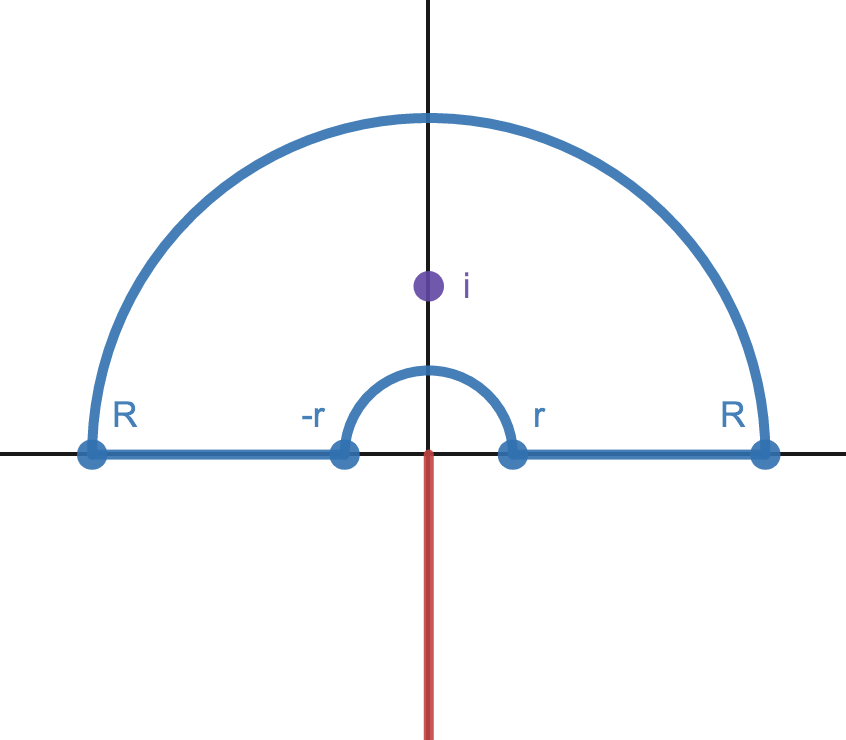
\includegraphics[width = 0.5\textwidth]{11.png}
        \caption{$\gamma$. Plotted in \cite{Desmos}.}
        \label{fig:fig11}
    \end{figure}
    Then by Residue Theorem, 
    \begin{align*}
        \i{\gamma}{}{f(z)}{z} & = 2\pi i n(\gamma;i) \Res(f;i) = 2\pi i \lim\limits_{z \to i} \sqbrack{ (z - i) f(z) } \\ 
        & = 2\pi i \lim\limits_{z \to i} \sqbrack{ \frac{(z-i) \Log(z)}{e^{\frac{1}{2}\Log(z)}(z - i)(z + i)}  } = 2\pi i \left. \sqbrack{ \frac{ \Log(z)}{e^{\frac{1}{2}\Log(z)}(z + i)} } \right|_{z = i} . 
    \end{align*}
    Then 
    \begin{align*}
        \Log(i) & = \Log \paren{ e^{\frac{\pi i}{2}} } = \ln(1) + \frac{\pi i}{2} = \frac{\pi i}{2} , \\ 
        e^{\frac{1}{2}\Log(z)} & = e^{\frac{\pi i}{4}} = \frac{1 + i}{\sqrt{2}} ,
    \end{align*}
    and so 
    \begin{align*}
        \i{\gamma}{}{f(z)}{z} & = 2\pi i  \sqbrack{ \frac{ \Log(i)}{e^{\frac{1}{2}\Log(i)}(i + i)} } = \frac{2\pi i}{2i} \cdot \frac{ \frac{\pi i}{2} }{ \frac{1 + i}{\sqrt{2}} } \\ 
        & = \frac{\pi^2 i\sqrt{2}}{2} \cdot \frac{1}{1 + i} \cdot \frac{1 - i}{1 - i} = \frac{\pi^2 i\sqrt{2}}{2} \cdot \frac{1 - i}{2} \\ 
        & = \frac{\pi^2 \sqrt{2}}{4} (1 + i) . 
    \end{align*}
    Thus 
    \begin{align*}
        \frac{\pi^2 \sqrt{2}}{4} (1 + i) & = \i{\gamma}{}{f(z)}{z} \\ 
        & = \i{[r,R]}{}{f(z)}{z} + \i{\gamma_R}{}{f(z)}{z} + \i{[-R,-r]}{}{f(z)}{z} + \i{\gamma_r}{}{f(z)}{z} , 
    \end{align*}
    where $\gamma_R$ and $\gamma_r$ are the semicircular arcs of $\gamma$ of radii $R$ and $r$, respectively. We evaluate each piece as follows. 
    
    The first integral is the easiest case. Simply parametrize $[r,R]$ by $r \leq x \leq R$, then 
    \[
        \i{[r,R]}{}{f(z)}{z} = \i{r}{R}{ \frac{\Log(x)}{e^{\frac{1}{2}\Log(x)} \paren{ 1 + x^2 } } }{x} = \i{r}{R}{ \frac{\ln(x)}{\sqrt{x} \paren{ 1 + x^2} }  }{x} . 
    \]
    The integral over $[-R,-r]$ is not as straightforward. Parametrize the integral by $-R \leq x \leq r$, where $x \in \real$ is negative, then 
    \[
        \i{[-R,-r]}{}{f(z)}{z} = \i{-R}{-r}{ \frac{\Log(x)}{e^{\frac{1}{2}\Log(x)} \paren{ 1 + x^2 } } }{x} . 
    \]
    Using 
    \[
        \Log(x) = \ln \paren{ \abs{x} } + \pi i 
    \]
    for $x < 0$, then 
    \begin{align*}
        e^{ \frac{1}{2} \Log(x) } & = e^{ \frac{1}{2} \sqbrack{ \ln \paren{ \abs{x} } + \pi i } } \\ 
        & = e^{ \frac{1}{2} \ln \paren{ \abs{x} } + \frac{\pi i}{2} } = e^{ \frac{1}{2} \ln \paren{ \abs{x} } } e^{ \frac{\pi i}{2} } \\ 
        & = \sqrt{ \abs{x} } i . 
    \end{align*}
    Thus 
    \begin{align*}
        \i{[-R,-r]}{}{f(z)}{z} & = \i{-R}{-r}{ \frac{\Log(x)}{e^{\frac{1}{2}\Log(x)} \paren{ 1 + x^2 } } }{x} = \i{-R}{-r}{ \frac{\ln \paren{ \abs{x} } + \pi i}{\sqrt{\abs{x}} i \paren{ 1 + x^2 } } }{x} \\ 
        & = -i \i{-R}{-r}{ \frac{\ln \paren{ \abs{x} } + \pi i}{\sqrt{\abs{x}} \paren{ 1 + x^2 } } }{x} \\ 
        & = -i \i{-R}{-r}{ \frac{ \ln \paren{ \abs{x} } }{ \sqrt{ \abs{x} } \paren{ 1 + x^2} } }{x} + \pi \i{-R}{-r}{ \frac{ 1 }{ \sqrt{ \abs{x} } \paren{ 1 + x^2} } }{x} .
    \end{align*}
    Since both integrands are even, we have 
    \begin{align*}
        \i{[-R,-r]}{}{f(z)}{z} & = -i \i{-R}{-r}{ \frac{ \ln \paren{ \abs{x} } }{ \sqrt{ \abs{x} } \paren{ 1 + x^2} } }{x} + \pi \i{-R}{-r}{ \frac{ 1 }{ \sqrt{ \abs{x} } \paren{ 1 + x^2} } }{x} \\ 
        & = -i \i{r}{R}{ \frac{ \ln(x) }{ \sqrt{ x } \paren{ 1 + x^2} } }{x} + \pi \i{r}{R}{ \frac{ 1 }{ \sqrt{ x } \paren{ 1 + x^2} } }{x} . 
    \end{align*}
    Next, we show that the integrals over $\gamma_R$ and $\gamma_r$ vanish as $R \to \infty$ and $r \to 0$, respectively. First, parametrize $\gamma_R$ by $\gamma_R(t) \coloneqq Re^{it}$, $0 \leq t \leq \pi$. Then 
    \begin{align*}
        \abs{ \i{\gamma_R}{}{f(z)}{z} } & = \abs{ \i{0}{\pi}{ \frac{ \Log \paren{ Re^{it} } }{ e^{ \frac{1}{2}  \Log \paren{ Re^{it} } } \paren{ 1 + R^2 e^{2it} } } iR e^{it} }{t} } \leq \i{0}{\pi}{ \abs{ \frac{ \Log \paren{ Re^{it} } }{ e^{ \frac{1}{2}  \Log \paren{ Re^{it} } } \paren{ 1 + R^2 e^{2it} } } iR e^{it} } }{t} \\ 
        & = R \i{0}{\pi}{ \frac{ \abs{ \ln(R) + it } }{ \abs{ e^{ \frac{1}{2} \sqbrack{ \ln(R) + it } } } \abs{ 1 + R^2 e^{2it} } } }{t} \leq R \i{0}{\pi}{ \frac{ \abs{ \ln(R) } + \abs{ it } }{ e^{ \frac{1}{2} \ln(R) } \abs{ 1 + R^2 e^{2it} } } }{t} \\ 
        & = R \i{0}{\pi}{ \frac{\ln(R) + t}{\sqrt{R} \abs{ 1 + R^2 e^{2it} }} }{t} \leq \sqrt{R} \i{0}{\pi}{ \frac{\ln(R) + \pi}{ \abs{ 1 + R^2 e^{2it} } } }{t} \\ 
        & \leq \sqrt{R} \sqbrack{ \ln(R) + \pi } \i{0}{\pi}{ \frac{1}{R^2 - 1} }{t} = \frac{\pi \sqrt{R} \sqbrack{ \ln(R) + \pi } }{R^2 -1} \\
        & = \mathcal{O} \paren{ \frac{\sqrt{R} \ln(R)}{R^2} } = \mathcal{O} \paren{ \frac{\ln(R)}{R^{\frac{3}{2}}} } \to 0
    \end{align*}
    as $R \to \infty$. For the integral over $\gamma_r$, parametrize as $\gamma_r(t) \coloneqq re^{-it}$, $0 \leq t \leq \pi$. We can employ the same bounds as for $\gamma_R$ to get 
    \[
        \abs{ \i{\gamma_r}{}{f(z)}{z} } \leq \sqrt{r} \i{0}{\pi}{ \frac{ \ln(r) + \pi }{ r^2 - 1 } }{t} . 
    \]
    However, blindly following the same bounds from here results in a term that diverges as $r \to 0$. Instead, note that $\ln(r) + \pi \leq \pi$ for all $r \leq 1$, and so 
    \begin{align*}
        \abs{ \i{\gamma_r}{}{f(z)}{z} } & \leq \sqrt{r} \i{0}{\pi}{ \frac{ \ln(r) + \pi }{ r^2 - 1 } }{t} \leq \sqrt{r} \i{0}{\pi}{ \frac{ \pi }{ r^2 - 1 } }{t} \\ 
        & = \frac{\pi^2 \sqrt{r}}{r^2 - 1} \to 0 
    \end{align*}
    as $r \to 0$. Then we can finally put the results together and take $R \to \infty$ and $r \to 0$ to get 
    \begin{align*}
        \frac{\pi^2 \sqrt{2}}{4} (1 + i) & = \i{[r,R]}{}{f(z)}{z} + \i{\gamma_R}{}{f(z)}{z} + \i{[-R,-r]}{}{f(z)}{z} + \i{\gamma_r}{}{f(z)}{z} , \\ 
        \Rightarrow \frac{\pi^2 \sqrt{2}}{4} (1 + i) & = \i{0}{\infty}{ \frac{\ln(x)}{\sqrt{x} \paren{1 + x^2} } }{x} + 0 - i \i{0}{\infty}{ \frac{\ln(x)}{\sqrt{x} \paren{1 + x^2} } }{x} \\ 
        & + \pi \underbrace{ \i{0}{\infty}{ \frac{1}{\sqrt{x}\paren{1+x^2}} }{x} }_{\eqqcolon J} + 0 \\ 
        & = (1 - i) I + \pi J , \\ 
        \Rightarrow I & = \frac{1 + i}{1+ i} \cdot \frac{1}{1 - i} \sqbrack{ \frac{\pi^2 \sqrt{2}}{4} (1 + i) - \pi J }  = \frac{1}{2} \sqbrack{ \frac{\pi^2\sqrt{2}}{4} (1 + 2i - 1) -\pi(1 + i) J } \\ 
        & = \frac{\pi^2 \sqrt{2}}{4} i - \frac{\pi }{2} (1 + i) J .
    \end{align*}
    Unfortunately we have to evaluate the integral 
    \[
        J = \i{0}{\infty}{ \frac{1}{\sqrt{x}\paren{1+x^2}}}{x} .
    \]
    Letting 
    \[
        g(z) \coloneqq \frac{1}{ e^{ \frac{1}{2} \Log(z) } \paren{ 1 + z^2 } } , 
    \]
    then $g$ is meromorphic on $\Omega$ with a simple poles at $z = i$. Then using the same contour $\gamma$, we have 
    \begin{align*}
        \i{\gamma}{}{g(z)}{z} & = 2\pi i n(\gamma;i) \Res(g;i) = 2\pi i \cdot \frac{\sqrt{2}}{(1+i)(2i)} \\ 
        & = \frac{\pi\sqrt{2}}{1 + i} \cdot \frac{1 - i}{1 - i} = \frac{\pi \sqrt{2}}{2}(1 - i) . 
    \end{align*}
    Then we can split up the integral as before and apply much of the same techniques: 
    \begin{align*}
        J & = \lim\limits_{ \substack{ r \to 0 \\ R \to \infty } }\i{[r,R]}{}{g(z)}{z} , \\ 
        \lim\limits_{R \to \infty} \abs{ \i{\gamma_R}{}{g(z)}{z} } & \leq \lim\limits_{R \to \infty} \frac{\pi \sqrt{R}}{R^2 - 1} \to 0 , \\ 
        \lim\limits_{ \substack{ r \to 0 \\ R \to \infty } } \i{[-R,-r]}{}{g(z)}{z} & = \lim\limits_{ \substack{ r \to 0 \\ R \to \infty } } -i \i{r}{R}{ \frac{1}{\sqrt{x}\paren{1+x^2}} }{x} = -i J , \\ 
        \lim\limits_{r \to 0} \abs{ \i{\gamma_r}{}{g(z)}{z} } & \leq \lim\limits_{r \to \infty} \frac{\pi \sqrt{r}}{r^2 - 1} \to 0 . 
    \end{align*}
    Then 
    \begin{align*}
        \frac{\pi \sqrt{2}}{2}(1 - i) & = \lim\limits_{ \substack{ r \to 0 \\ R \to \infty } }\i{\gamma}{}{g(z)}{z} = J + 0 -iJ + 0 , \\ 
        \Rightarrow J & = \frac{\pi \sqrt{2}}{2} . 
    \end{align*}
    Finally, 
    \begin{align*}
        I & = \frac{\pi^2 \sqrt{2}}{4} i - \frac{\pi }{2} (1 + i) J = \frac{\pi^2 \sqrt{2}}{4} i - \frac{\pi }{2} (1 + i) \frac{\pi \sqrt{2}}{2} \\ 
        & = \frac{\pi^2 \sqrt{2}}{4} i - \frac{\pi^2 \sqrt{2}}{4} - \frac{\pi^2 \sqrt{2}}{4} i = \boxed{ - \frac{\pi^2 \sqrt{2}}{4} . }
    \end{align*}
\end{proof}
\subsection{Problem 4}
Suppose that $f$ is analytic in the unit disk with a zero of order $m \geq 2$ at $z = 0$. Let 
\[
    g = \frac{f'''}{f'} - \frac{3}{2} \paren{ \frac{f''}{f'} }^2.
\]
Prove that in a neighborhood of $z = 0$, $g$ has a Laurent expansion of the form
\[
    g(z) = \sum\limits_{k = -2}^{\infty} a_k z^k
\]
with 
\[
    a_{-2} = \frac{1}{2} (1-m^2). 
\]
\begin{proof}[Answer]
    Since $f$ has a zero at $z = 0$ of order $m \geq 2$, in a neighborhood $U \subseteq B(0;1)$ of $z = 0$ we can write 
    \[
        f(z) = z^m h(z) , 
    \]
    where $h$ is analytic and nonzero on $U$. Then 
    \begin{align*}
        f'(z) & = m z^{m-1} h(z) + z^m h'(z) = z^{m-1} \sqbrack{ m h(z) + z h'(z) } , \\ 
        f''(z) & = m(m-1) z^{m-2} h(z) + m z^{m-1} h'(z) + m z^{m-1} h'(z) + z^m h''(z) \\ 
        & = z^{m-2} \sqbrack{ m(m-1)h(z) + 2mz h'(z) + z^2 h''(z) } , \\ 
        f'''(z) & = m(m-1)(m-2) z^{m-3} h(z) + m(m-1) z^{m-2} h'(z) \\ 
        & + 2m(m-1) z^{m-2} h'(z) + 2m z^{m-1} h''(z) \\ 
        & + m z^{m-1} h''(z) + z^m h'''(z) \\ 
        & = z^{m-3} \sqbrack{ m(m-1)(m-2) h(z) + 3m(m-1) z h'(z) + 3m z^2 h''(z) + z^3 h'''(z) } . 
    \end{align*}
    Now, write 
    \[
        \frac{f'''(z)}{f'(z)} = \frac{1}{z^2} \underbrace{ \sqbrack{ \frac{m(m-1)(m-2) h(z) + 3m(m-1) z h'(z) + 3m z^2 h''(z) + z^3 h'''(z)}{ m h(z) + z h'(z) } } }_{ \eqqcolon h_1(z) } .
    \]
    Then $h_1$ is meromorphic on $U$ and as 
    \begin{align*}
        h_1(0) & = \frac{m(m-1)(m-2) h(0) + 3m(m-1) \cdot 0 \cdot h'(0) + 3m \cdot 0^2 \cdot h''(0) + 0^3 \cdot h'''(0)}{m h(0) + 0 \cdot h'(0)} \\ 
        & = \frac{m(m-1)(m-2) h(0)}{mh(0)} = (m-1)(m-2) , 
    \end{align*}
    and so shrinking $U$ if necessary, $h_1$ is analytic on $U$. Thus we can write 
    \[
        h_1(z) = \sum\limits_{n = 0}^{\infty} b_n z^n , 
    \]
    where 
    \[
        b_0 = h(0) = (m-1)(m-2) . 
    \]
    Next, write 
    \[
        \frac{f''(z)}{f'(z)} = \frac{1}{z} \underbrace{ \sqbrack{ \frac{ m(m-1) h(z) + 2m z h'(z) + z^2 h''(z) }{ m h(z) + z h'(z) } } }_{ \eqqcolon h_2(z) } . 
    \]
    Again, $h_2$ is meromorphic on $U$ and as 
    \begin{align*}
        h_2(0) & = \frac{ m(m-1) h(0) + 2m \cdot 0 \cdot h'(0) + 0^2 \cdot h''(0) }{ m h(0) + 0 \cdot h'(z) } \\ 
        & = \frac{m(m-1)h(0)}{mh(0)} = m-1 \neq 0 . 
    \end{align*}
    Then shrinking $U$ again if necessary, $h_2$, and in turn $h_2^2$, is analytic and nonzero on $U$, and we can write 
    \[
        h_2(z)^2 = \sum\limits_{n = 0}^{\infty} c_n z^n , 
    \]
    where 
    \[
        c_0 = h_2(0)^2 = (m-1)^2 \neq 0 . 
    \]
    Then 
    \begin{align*}
        g(z) & = \frac{f'''(z)}{f'(z)} - \frac{3}{2} \sqbrack{ \frac{f''(z)}{f'(z)} }^2 = \frac{h_1(z)}{z^2} - \frac{3 h_2(z)^2 }{2z^2} \\ 
        & = \frac{1}{z^2} \sqbrack{ h_1(z) - \frac{3}{2} h_2(z)^2 } ,
    \end{align*}
    and so 
    \begin{align*}
        h_1(0) - \frac{3}{2} h_2(0)^2 & = (m-1)(m-2) - \frac{3}{2} (m-1)^2 = m^2 - m -2m + 2 - \frac{3}{2} \paren{ m^2 - 2m + 1 } \\ 
        & = m^2 - 3m + 2 - \frac{3}{2} m^2 + 3m - \frac{3}{2} = -\frac{1}{2}m^2 + \frac{1}{2} \\ 
        & = \frac{1 - m^2}{2} .
    \end{align*}
    Thus we can write 
    \begin{align*}
        g(z) & = \frac{1}{z^2} \sqbrack{ h_1(z) - \frac{3}{2} h_2(z)^2 } = \frac{1}{z^2} \sqbrack{ \frac{1 - m^2}{2} + \mathcal{O}(z) } \\ 
        & = \frac{1 - m^2}{z^2} + \frac{a_{-1}}{z} + a_0 + \mathcal{O}(z) = \sum\limits_{k = -2}^{\infty} a_{k} z^k , 
    \end{align*}
    where 
    \[
        a_{-2} = \frac{1 - m^2}{z^2} . \, \checkmark
    \]
\end{proof}

\newpage

\newpage
\section{Fall 2021 [Answered]}
Answer three complete questions in each of the two sections Real Analysis, Complex Analysis. Each problem is worth 10 points. You must fully justify all of your answers in order to get full credit. 

\subsection{Problem 1}
Is the function $z \mapsto \overline{z}$ analytic in $\cx$? State a yes/no answer and prove it. 
\begin{proof}[Answer]
    Let $f : \cx \to \cx$, $f(z) \coloneqq \bar{z}$. There are several ways to show that $f$ is not analytic, here we will show that $f'(z)$ does not exist for any $z \in \cx$. Consider 
    \[
        \lim\limits_{h \to 0} \frac{f(z + h) - f(z)}{h} = \lim\limits_{h \to 0} \frac{\overline{z + h} - \bar{z}}{h} = \lim\limits_{h \to 0} \frac{\bar{z} - \bar{h} - \bar{z}}{h} = \lim\limits_{h \to 0} \frac{\bar{h}}{h} . 
    \]
    Thus it suffices to show that the limit 
    \[
        \lim\limits_{h \to 0} \frac{\bar{h}}{h}
    \]
    does not exist. Taking the limit along the real axis, set $h = x$ for some $x \in \real$. Then 
    \[
        \lim\limits_{h \to 0} \frac{\bar{h}}{h} = \lim\limits_{x \to 0} \frac{\bar{x}}{x} = \lim\limits_{x \to 0} \frac{x}{x} = 1 . 
    \]
    However, if we take the limit along the imaginary axis, then, setting $h = iy$ for some $y \in \real$, 
    \[
        \lim\limits_{h \to 0} \frac{\bar{h}}{h} = \lim\limits_{y \to 0} \frac{\bar{iy}}{iy} = \lim\limits_{y \to 0} \frac{-iy}{iy} = -1 . 
    \]
    Thus the two limits are not equal, and so the limit does not exist. 
    
    The conjugate map is an easy example to pick on for a non-analytic map, despite its rather outstanding qualities: it is a homeomorphism and a field automorphism. 
\end{proof}

\subsection{Problem 2 \texorpdfstring{\cite{Evan}}{}}
Let 
\[
    f(z) = \sum\limits_{n = 0}^{\infty} c_n z^n
\]
be analytic in the entire $\cx$ and let there exist a finite constant $C$ such that 
\[
    \abs{f(z)} \leq C e^{|z|} \quad \forall z \in \cx . 
\]
Prove that 
\[
    \abs{ c_n } \leq C \paren{ \frac{e}{n} }^n
\]
for all $n = 1, 2, ...$. 
\begin{proof}[Answer]
    Since $f$ is entire, the coefficients $c_k$ are given by 
    \[
        c_k = \frac{n(\gamma;0)}{2\pi i} \i{\gamma}{}{ \frac{f(z)}{z^{k+1}} }{z}
    \]
    for any simple closed (rectifiable) curve $\gamma$ encircling the origin. In particular, for each $k \in \n$, we can take 
    \[
        c_k = \frac{n(\gamma;0)}{2\pi i} \i{\gamma_k}{}{ \frac{f(z)}{z^{k+1}} }{z}
    \]
    where $\gamma_k(t) \coloneqq k e^{it}$, $0 \leq t \leq 2\pi$. Then 
    \begin{align*}
        \abs{ c_k } & = \abs{ \frac{n \paren{ \gamma_k;0 }}{2\pi i} \i{\gamma_k}{}{ \frac{f(z)}{z^{k+1}} }{z} } = \frac{1}{2\pi} \abs{ \i{0}{2\pi}{ \frac{ f \paren{ k e^{it} } }{ k^{k+1} e^{i(k+1)t} } i e^{it}}{t} } \\
        & \leq \frac{1}{2\pi} \i{0}{2\pi}{ \abs{ \frac{ f \paren{ k e^{it} } }{ k^{k+1} e^{ikt} } i e^{it} } }{t} = \frac{k}{2\pi k^{k+1}} \i{0}{2\pi}{ \abs{ f \paren{ k e^{it} } } }{t} \\ 
        & \leq \frac{1}{2\pi k^{k}} \i{0}{2\pi}{ C e^{\abs{ke^{it}}} }{t} = \frac{1}{2\pi k^{k}} \i{0}{2\pi}{ C e^{k} }{t} \\ 
        & = \frac{2\pi}{2\pi k^k} C e^k = C \paren{ \frac{e}{k} }^k . \, \checkmark 
    \end{align*}
\end{proof}

\subsection{Problem 3 \texorpdfstring{\cite{Lang}}{}}
Find the Laurent expansion of the function $(z + i)/z^2$ in an annulus $D$ centered at $i$ containing $-i$. What is the maximal annulus in which your expansion holds? Prove your answer. 
\begin{proof}[Answer]
    Let 
    \[
        f(z) \coloneqq \frac{z + i}{z} = \frac{1}{z} + \frac{i}{z^2}
    \]
    for $z \in \cx$. Then $f$ is meromorphic on $\cx$ with a double pole at $z = 0$. First, rewrite $\frac{1}{z}$ as 
    \begin{align*}
        \frac{1}{z} & = \frac{1}{z - i + i} = \frac{1}{i + \paren{ z - i }} \\ 
        & = \frac{1}{z - i} \cdot \frac{1}{ \frac{i}{z - i} + 1 } = \frac{1}{z - i} \cdot \frac{1}{ 1 - \paren{ \frac{-i}{z - i} } } \\ 
        & = \frac{1}{z - i} \sum\limits_{n = 0}^{\infty} \paren{ \frac{-i}{z - i} } = \sum\limits_{n = 0}^{\infty} \frac{(-i)^n}{(z-i)^{n+1}} \\ 
        & = \sum\limits_{m = 1}^{\infty} (-i)^{m-1} (z - i)^{-m} , 
    \end{align*}
    which converges for 
    \begin{align*}
        1 & > \abs{ \frac{-i}{z - i} } = \frac{1}{\abs{z-i}}\\ 
        \Rightarrow \abs{z-i} & > 1 .
    \end{align*}
    Let 
    \[
        D \coloneqq \setb{ z \in \cx \, \middle| \, \abs{z - i} > 1 } , 
    \]
    then $D$ is an annulus centered at $i$ which contains $-i$. Then \[
        \frac{1}{z^2} = \paren{ \frac{1}{z} }^2 = \sqbrack{ \sum\limits_{m = 1}^{\infty} (-i)^{m-1} (z - i)^{-m} }^2 = \sum\limits_{m = 1}^{\infty} c_m \paren{ z - i }^{-m}, 
    \]
    where the coefficients $c_m$ are given by the Cauchy product
    \begin{align*}
        c_m & = \sum\limits_{j = 1}^{m-1} (-i)^{j-1} (-i)^{m-1-j} = \sum\limits_{j = 1}^{m-1} (-i)^{m-2} \\ 
        & = (m-1-1+1) (-i)^{m-2} = (m-1) (-i)^{-1} (-i)^{m-1} \\ 
        & = -(m-1) (-i)^{m-1} .
    \end{align*}
    Thus 
    \[
        \frac{1}{z^2} = \sum\limits_{m = 1}^{\infty} c_m \paren{ z - i }^{-m} = \sum\limits_{m = 1}^{\infty} -(m-1) (-i)^{m-1} \paren{ z - i }^{-m}
    \]
    on $D$, and so 
    \begin{align*}
        f(z) & = \frac{1}{z} + \frac{i}{z^2} = \sum\limits_{m = 1}^{\infty} (-i)^{m-1} (z - i)^{-m} + i \sum\limits_{m = 1}^{\infty} -(m-1) (-i)^{m-1} \paren{ z - i }^{-m} \\ 
        & = \sum\limits_{m = 1}^{\infty} \sqbrack{ 1 - i(m-1) } (-i)^{m-1} z^{-m} 
    \end{align*}
    for $z \in D$. Now, since $D$ is unbounded, any larger annulus centered at $i$ that contains $-i$ will include a $z \in \cx$ that satisfies $\abs{z - i} < 1$. But since the series diverges for $\abs{ z - i } < 1$, the above expansion cannot converge on any larger annulus centered at $i$ containing $-i$. Thus $D$ is the maximal annulus for which the expansion holds. 
\end{proof}

\subsection{Problem 4}
Let $f : \cx \to \cx$ be continuous at every point. Let $f$ be analytic in the domains $D_1 = \setb{z : \im z > 0 }$ and $D_2 = \setb{ z : \im z < 0 }$. Prove that $f$ is analytic in $\cx$. 
\begin{proof}[Answer]
    We show that $f$ is entire by using Morera's Theorem. It suffices to use rectangles with sides parallel to the real and imaginary axes. Let $R$ be such a rectangle. If $R$ is contained in either the upper or lower half planes, then as $f$ is analytic on $\cx \setminus \real$, 
    \[
        \i{R}{}{f(z)}{z} = 0 
    \]
    by Cauchy's Theorem. Now, suppose that $R$ intersects the real axis. We specialize to the case of the boundary of the square $[-1,1]^2$, but the same techniques generalize to any rectangle under consideration. 
    
    Let $R$ be the boundary curve of the square $[-1,1]^2$, oriented counterclockwise. Then we can write 
    \[
        \i{R}{}{f(z)}{z} = \i{R_1}{}{f(z)}{z} + \i{R_2}{}{f(z)}{z}
    \]
    where $R_1$ and $R_2$ are the rectangles as pictured below:
    \begin{figure}[H]
        \centering
        \begin{subfigure}{0.45\textwidth}
            \centering
            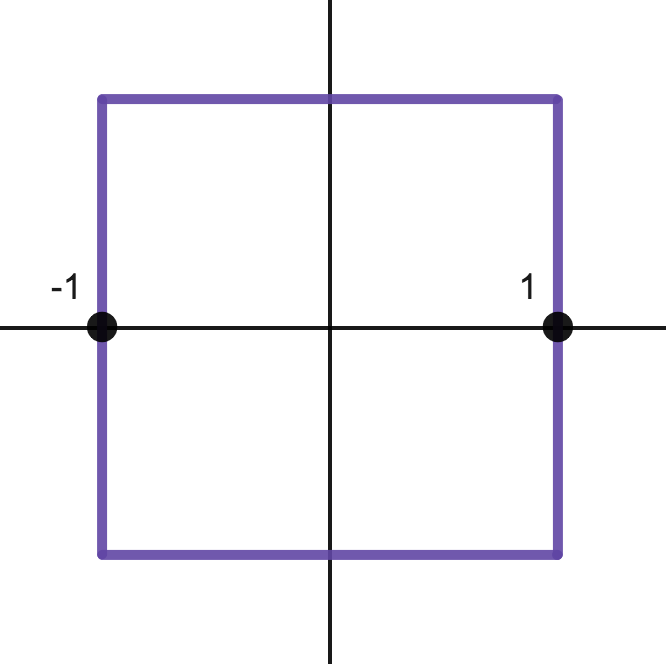
\includegraphics[width=\textwidth]{12a.png}
            \subcaption{$R$.}
            \label{fig:12a}
        \end{subfigure}
        \hfill
        \begin{subfigure}{0.45\textwidth}
            \centering
            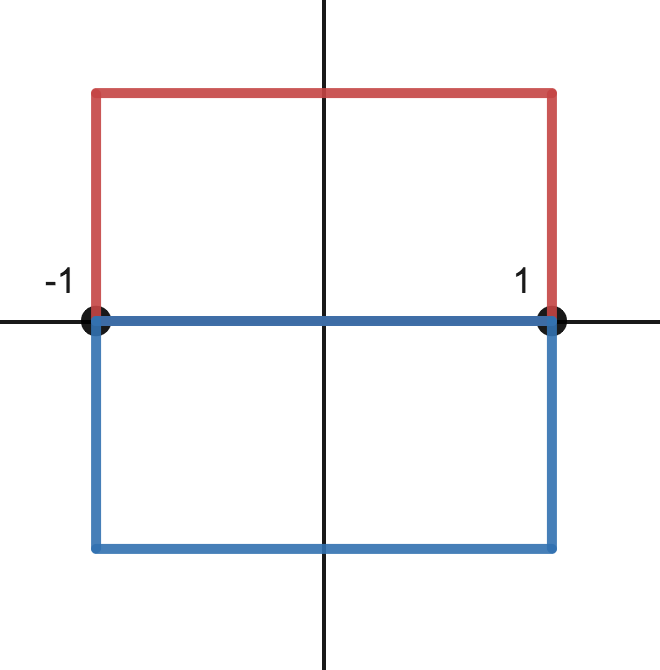
\includegraphics[width=\textwidth]{12b.png}
            \subcaption{$R_1$ (red) and $R_2$ (blue).}
            \label{fig:12b}
        \end{subfigure}
        \caption{Plotted in \cite{Desmos}.}
    \end{figure}
    UNFINISHED
\end{proof}

\newpage 
\section{Extra}
\subsection{Practice with Residues \texorpdfstring{\cite{Conway,Ryan}}{}}
In preparing for this qual, I worked through several examples of computing integrals with residues from \cite{Conway}. 
\begin{enumerate}
    \item Show that 
    \[
        \int_{-\infty}^{\infty} \frac{x^2}{1+x^4} \, \mathrm{d}x = \frac{\pi}{\sqrt{2}}.
    \]
    \begin{proof}[Answer]
        Let 
        \[
            f(z) \coloneqq \frac{z^2}{1 + z^4},
        \]
        then $f$ is meromorphic with poles 
        \[
            a_1 = \frac{1 + i}{\sqrt{2}} , \quad a_2 = \frac{-1 + i}{\sqrt{2}} , \quad a_3 = -a_1 , \quad a_4 = -a_2,
        \]
        each of order 1. Let $R > 1$, and let $\gamma$ be the upper semicircle of radius $R$ centered at the origin, oriented counterclockwise. Note that $\gamma$ encircles $a_1$ and $a_2$, and so by Residue Theorem
        \[
            \int_{\gamma} f(z) \, \mathrm{d}z = 2\pi i \sqbrack{ \Res(f;a_1) + \Res(f;a_2) }.
        \]
        Then 
        \begin{align*}
            \Res(f;a_1) & = \lim\limits_{z \to a_1} (z-a_1) f(z) \\
            & = \lim\limits_{z \to a_1} \frac{(z - a_1)z^2}{(z-a_1)(z-a_2)(z+a_1)(z+a_2)} \\
            & = \left. \frac{z^2}{(z-a_2)(z+a_1)(z+a_2)} \right|_{z = a_1} \\
            & = \frac{a_1^2}{(a_1 - a_2)(a_1 + a_1)(a_1 + a_2)}.
        \end{align*}
        Note that $a_1 - a_2 = \frac{2}{\sqrt{2}} = \sqrt{2}$, and $a_1 + a_2 = \frac{2i}{\sqrt{2}} = \sqrt{2}i$. Thus 
        \begin{align*}
            \Res(f;a_1) & = \frac{ a_1^2 }{ \paren{ \sqrt{2} } \paren{ 2a_1 } \paren{ \sqrt{2}i } } = -\frac{i}{4}a_1 \\
            & = \frac{1 - i}{4\sqrt{2}} = -\frac{a_2}{4}.
        \end{align*}
        Next,
        \begin{align*}
            \Res(f;a_2) & = \lim\limits_{z \to a_2} (z-a_2) f(z) \\
            & = \lim\limits_{z \to a_2} \frac{(z - a_2)z^2}{(z-a_1)(z-a_2)(z+a_1)(z+a_2)} \\
            & = \left. \frac{z^2}{(z-a_1)(z+a_1)(z+a_2)} \right|_{z = a_2} \\
            & = \frac{a_2^2}{(a_2-a_1)(a_2+a_1)(a_2+a_2)} \\
            & = \frac{a_2^2}{(-\sqrt{2})(\sqrt{2}i)(2a_2)} = \frac{i}{4}a_2 \\
            & = \frac{-1 - i}{4\sqrt{2}} = -\frac{a_1}{4}.
        \end{align*}
        Thus 
        \begin{align*}
            \int_{\gamma} f(z) \, \mathrm{d}z & = 2\pi i \sqbrack{ \Res(f;a_1) + \Res(f;a_2) } \\
            & = 2\pi i \paren{ -\frac{a_2}{4} - \frac{a_1}{4} } = -\frac{\pi i}{2}(a_1 + a_2) \\
            & = -\frac{\pi i}{2} \times \sqrt{2} i = \frac{\pi}{\sqrt{2}}.
        \end{align*}
        Then 
        \[
            \int_{\gamma} f(z) \, \mathrm{d}z = \int_{-R}^R \frac{x^2}{1+x^4} \, \mathrm{d}x + \underbrace{ \int_0^{\pi} \frac{ R^2 e^{2it} }{ 1 + R^4 e^{4it} } iRe^{it} \, \mathrm{d}t }_{ \eqqcolon I(R) }.
        \]
        We show that $|I(R)| \to 0$ as $R \to \infty$, then $\lim\limits_{R \to \infty} I(R) = 0$. Note that 
        \begin{align*}
            0 & \leq |I(R)| \leq \left| \int_0^{\pi} \frac{ iR^3 e^{3it} }{ 1 + R^4 e^{4it} } \, \mathrm{d}t \right| \\
            & = R^3 \left| \int_0^{\pi} \frac{ e^{3it} }{ 1 + R^4 e^{4it} } \, \mathrm{d}t \right| leq R^3 \int_0^{\pi} \left|  \frac{ e^{3it} }{ 1 + R^4 e^{4it} } \right| \, \mathrm{d}t \\
            & = R^3 \int_0^{\pi} \frac{ |e^{3it}| }{ |1 + R^4 e^{4it}| } \, \mathrm{d}t = R^3 \int_0^{\pi} \frac{ 1 }{ |1 + R^4 e^{4it}| } \, \mathrm{d}t.
        \end{align*}
        By the Triangle Inequality
        \begin{align*}
            \left| -1 + 1 + R^4e^{4it} \right| & \leq |-1| + \left| 1 + R^4e^{4it} \right| \\
            \left| R^4e^{4it} \right| & \leq R^4 \leq 1 + \left| 1 + R^4e^{4it} \right| \\ 
            \left| 1 + R^4e^{4it} \right| & \geq R^4 - 1.
        \end{align*}
        Then 
        \begin{align*}
            |I(R)| & \leq R^3 \int_0^{\pi} \frac{ 1 }{ |1 + R^4 e^{4it}| } \, \mathrm{d}t \leq R^3 \int_0^{\pi} \frac{1}{R^4 - 1} \, \mathrm{d}t \\
            & = \frac{\pi R^3}{R^4 - 1} \to 0
        \end{align*}
        as $R \to \infty$. Then 
        \begin{align*}
            \lim\limits_{R \to \infty} \int_{-R}^R \frac{x^2}{1+x^4} \, \mathrm{d}x & = \int_{-\infty}^{\infty} \frac{x^2}{1+x^4} \, \mathrm{d}x == \lim\limits_{R \to \infty} \sqbrack{ \int_{\gamma} f(z) \, \mathrm{d}z - I(R) } \\
            & = \frac{\pi}{\sqrt{2}} - 0 == \boxed{ \frac{\pi}{\sqrt{2}}. }
        \end{align*}
    \end{proof}
    \item Show that 
    \[
        \int_0^{\infty} \frac{\sin x}{x} \, \mathrm{d}x = \frac{\pi}{2}.
    \]
    \begin{proof}[Answer]
        Let 
        \[
            f(z) \coloneqq \frac{e^{iz}}{z},
        \]
        then $f$ has a simple pole at $z = 0$. Let $0 < r < R$, and let $\gamma$ be the curve given below, oriented counterclockwise.
        \begin{figure}[H]
            \centering
            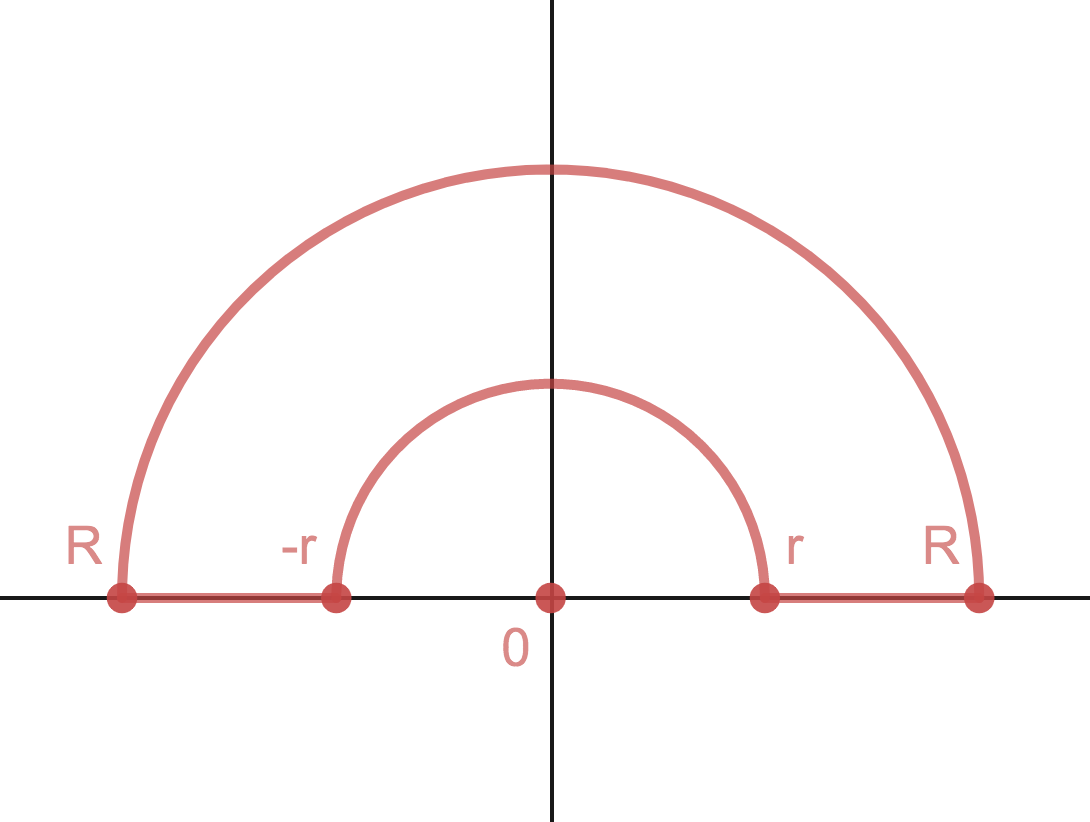
\includegraphics[width = 0.5\textwidth]{7}
            \caption{$\gamma$. Plotted in \cite{Desmos}.}
            \label{fig:fig7}
        \end{figure}
        By Cauchy's Theorem (take the region $f$ is defined on to be $\cx \setminus \setb{ 0 }$), 
        \[
            \int_{\gamma} f(z) \, \mathrm{d}z = \int_{\gamma} \frac{e^{iz}}{z} \, \mathrm{d}z = 0.
        \]
        So 
        \begin{align*}
            0 & = \int_{\gamma} \frac{e^{iz}}{z} \, \mathrm{d}z \\
            & = \int_r^R \frac{e^{ix}}{x} \, \mathrm{d}x + \int_{\gamma_R} \frac{e^{iz}}{z} \, \mathrm{d}z + \int_{-R}^{-r} \frac{e^{ix}}{x} \, \mathrm{d}x + \int_{\gamma_r} \frac{e^{iz}}{z} \, \mathrm{d}x.
        \end{align*}
        Note that 
        \begin{align*}
            \int_r^R \frac{ \sin x}{x} \, \mathrm{d}x & = \frac{1}{2i} \int_r^R \frac{e^{ix} - e^{-ix}}{x} \, \mathrm{d}x \\
            & = \frac{1}{2i} \int_r^R \frac{e^{ix}}{x} \, \mathrm{d}x - \frac{1}{2i} \int_r^R \frac{e^{-ix}}{x} \, \mathrm{d}x \\
            & = \frac{1}{2i} \int_r^R \frac{e^{ix}}{x} \, \mathrm{d}x + \frac{1}{2i} \int_{-R}^{-r} \frac{e^{ix}}{x} \, \mathrm{d}x.
        \end{align*}
        Then 
        \begin{align*}
            0 & = \int_r^R \frac{e^{ix}}{x} \, \mathrm{d}x + \int_{\gamma_R} \frac{e^{iz}}{z} \, \mathrm{d}z + \int_{-R}^{-r} \frac{e^{ix}}{x} \, \mathrm{d}x + \int_{\gamma_r} \frac{e^{iz}}{z} \, \mathrm{d}x \\
            & = 2i \int_r^R \frac{ \sin x}{x} \, \mathrm{d}x + \int_{\gamma_R} \frac{e^{iz}}{z} \, \mathrm{d}z + \int_{\gamma_r} \frac{e^{iz}}{z} \, \mathrm{d}z \\
            \int_r^R \frac{ \sin x}{x} \, \mathrm{d}x & = -\frac{1}{2i} \paren{ \int_{\gamma_R} \frac{e^{iz}}{z} \, \mathrm{d}z + \int_{\gamma_r} \frac{e^{iz}}{z} \, \mathrm{d}z }.
        \end{align*}
        Now, 
        \begin{align*}
            \left| \int_{\gamma_R} \frac{e^{iz}}{z} \, \mathrm{d}z \right| & = \left| \int_0^{\pi} \frac{ \exp \paren{ iR e^{i \theta} } }{ Re^{i \theta} } i R e^{i \theta} \, \mathrm{d}\theta \right| = \left| \int_0^{\pi} \exp \paren{ iR e^{i \theta} } \, \mathrm{d}\theta \right| \\
            & \leq \int_0^{\pi} \left| \exp \paren{ iR e^{i \theta} } \right| \, \mathrm{d} \theta = \int_0^{\pi} e^{ \re \paren{ iR e^{i \theta} } } \, \mathrm{d} \theta.
        \end{align*}
        Write $e^{i \theta} = \cos \theta + i \sin \theta$, then 
        \begin{align*}
            \re \paren{ iR e^{i \theta} } & = \re \sqbrack{ i R \paren{ \cos \theta + i \sin \theta } } \\
            & = \re \paren{ iR \cos \theta - R \sin \theta } \\
            & = -R \sin \theta.
        \end{align*}
        Thus 
        \[
            \left| \int_{\gamma_R} \frac{e^{iz}}{z} \, \mathrm{d}z \right| \leq \int_0^{\pi} e^{ \re \paren{ iR e^{i \theta} } } \, \mathrm{d} \theta = \int_0^{\pi} e^{ -R \sin \theta } \, \mathrm{d} \theta.
        \]
        \begin{claim}
            There exists $\delta > 0$ such that the maximum value of $e^{ -R \sin \theta }$ on $[\delta, \pi - \delta]$ is $e^{ -R \sin \delta }$.
        \end{claim}
        \begin{proof}
            Let $g : [0,\pi] \to \real$, $g(\theta) \coloneqq e^{ -R \sin \theta }$. $g$ is continuously differentiable on $(0,\pi)$. We find the extrema of $g$ on $[0,\pi]$. First, the endpoints:
            \begin{align*}
                g(0) & =  e^{ -R \sin(0) } = e^{-R \times 0} \\
                & = e^0 = 1, \\
                g(\pi) & =  e^{ -R \sin \paren{ \pi } } = e^{-R \times 0} \\
                & = 1.
            \end{align*}
            Next, we find critical points of $g$. 
            \[
                g'(\theta) = e^{-R \sin \theta} \cdot \paren{ -R \cos \theta } = -R e^{-R \sin \theta} \cos \theta.
            \]
            Then 
            \begin{align*}
                0 & = g'(\theta) = -R e^{-R \sin \theta} \cos \theta \\
                0 & = \cos \theta.
            \end{align*}
            Since $0 \leq \theta \leq \pi$, this gives us $\theta = \frac{\pi}{2}$ as a critical point. Then 
            \begin{align*}
                g' \paren{ \frac{\pi}{4} } & = -R e^{-R \paren{ \frac{\pi}{4} } } \cos \paren{ \frac{\pi}{4} } = -\frac{R \sqrt{2}}{2} e^{- \frac{R\sqrt{2}}{2} } < 0 , \\
                g' \paren{ \frac{3\pi}{4} } & = -R e^{-R \paren{ \frac{3\pi}{4} } } \cos \paren{ \frac{3\pi}{4} } = \frac{R \sqrt{2}}{2} e^{- \frac{R\sqrt{2}}{2} } > 0.
            \end{align*}
            Thus $g$ is decreasing on $ \paren{ 0 , \frac{\pi}{2} }$ and increasing on $\paren{ \frac{\pi}{2} , \pi }$. Therefore $\theta = \frac{\pi}{2}$ is the minimum of $g$ on $[0,\pi]$. Now, note that $g$ is symmetric about $\theta = \frac{\pi}{2}$, since
            \begin{align*}
                g \paren{ \frac{\pi}{2} + x } & = \exp \sqbrack{ -R \sin \paren{ \frac{\pi}{2} + x } } \\
                & = \exp \sqbrack{ -R \sin \paren{ \frac{\pi}{2} } \cos x - R \cos \paren{ \frac{\pi}{2} } \sin x } \\
                & = \exp \paren{ -R \cos x } = \exp \sqbrack{ R \cos \paren{ -x } } \\
                & = g \paren{ \frac{\pi}{2} - x }.
            \end{align*}
            \begin{figure}[H]
                \centering
                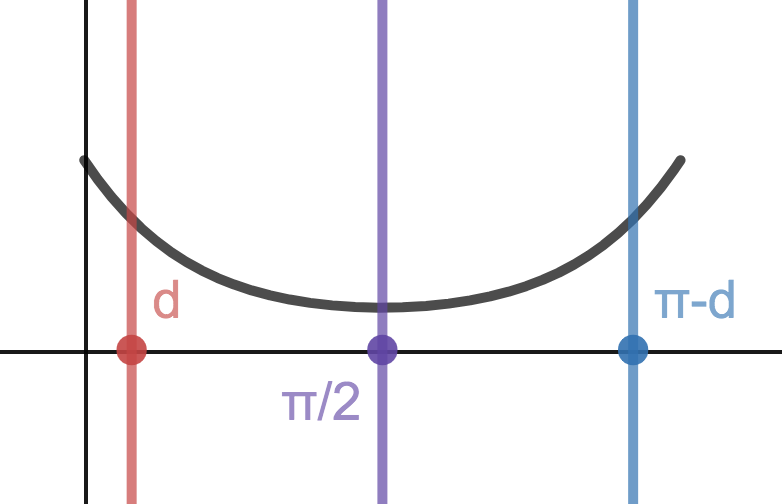
\includegraphics[width = 0.5\textwidth]{8.png}
                \caption{$g$. Plotted in \cite{Desmos}.}
                \label{fig:fig8}
            \end{figure}
            Thus for any $0 < \delta < \frac{\pi}{2}$, $g$ is decreasing on $\sqbrack{ \delta , \frac{\pi}{2} }$ and is increasing on $\sqbrack{ \frac{\pi}{2} , \pi - \delta }$. Thus the maximum of $g$ on $\sqbrack{ \delta , \pi - \delta }$ is 
            \[
                g(\delta) = g(\pi - \delta) = e^{-R \sin \delta}.
            \]
        \end{proof}
        Thus 
        \begin{align*}
            \left| \int_{\gamma_R} \frac{e^{iz}}{z} \, \mathrm{d}z \right| & \leq \int_0^{\pi} e^{ -R \sin \theta } \, \mathrm{d} \theta \\
            & = \int_0^{\delta} e^{ -R \sin \theta } \, \mathrm{d} \theta + \int_{\delta}^{\pi-\delta} e^{ -R \sin \theta } \, \mathrm{d} \theta + \int_{\pi - \delta}^{\pi} e^{ -R \sin \theta } \, \mathrm{d} \theta \\
            & \leq \int_0^{\delta} e^{ -R \sin \theta } \, \mathrm{d} \theta + \paren{ \pi - 2 \delta } e^{-R \sin \delta } + \int_{\pi - \delta}^{\pi} e^{ -R \sin \theta } \, \mathrm{d} \theta.
        \end{align*}
        Since $e^{ -R \sin \theta }$ is symmetric about $\theta = \frac{\pi}{2}$, we can write 
        \begin{align*}
            \left| \int_{\gamma_R} \frac{e^{iz}}{z} \, \mathrm{d}z \right| & \leq \int_0^{\delta} e^{ -R \sin \theta } \, \mathrm{d} \theta + \paren{ \pi - 2 \delta } e^{-R \sin \delta } + \int_{\pi - \delta}^{\pi} e^{ -R \sin \theta } \, \mathrm{d} \theta \\
            & = \int_0^{\delta} e^{ -R \sin \theta } \, \mathrm{d} \theta + \paren{ \pi - 2 \delta } e^{-R \sin \delta } + \int_{0}^{\delta} e^{ -R \sin \theta } \, \mathrm{d} \theta \\
            & = 2\int_0^{\delta} e^{ -R \sin \theta } \, \mathrm{d} \theta + \paren{ \pi - 2 \delta } e^{-R \sin \delta }.
        \end{align*}
        From the proof of the above claim, we found that the maximum value of $e^{-R \sin \theta}$ on $[0,\pi]$ is 1. Thus 
        \begin{align*}
            \left| \int_{\gamma_R} \frac{e^{iz}}{z} \, \mathrm{d}z \right| & \leq 2\int_0^{\delta} e^{ -R \sin \theta } \, \mathrm{d} \theta + \paren{ \pi - 2 \delta } e^{-R \sin \delta } \\
            & \leq 2 \delta + \paren{ \pi - 2 \delta } e^{-R \sin \delta } \\
            & = 2 \delta \paren{ 1 - e^{-R \sin \delta} } + \pi e^{-R \sin \delta}.
        \end{align*}
        Since $0 < \delta < \frac{\pi}{2}$, $ \sin \delta > 0$, and so $e^{-R \sin \delta } < 1$. Hence
        \[
            \left| \int_{\gamma_R} \frac{e^{iz}}{z} \, \mathrm{d}z \right| \leq 2 \delta \paren{ 1 - e^{-R \sin \delta} } + \pi e^{-R \sin \delta} < 2 \delta + \pi e^{-R \sin \delta}.
        \]
        Given $\epsilon > 0$, choose $\delta < \min \setb{ \frac{\epsilon}{3} , \frac{\pi}{2} }$. Since $e^{-R \sin \delta} \to 0$ as $R \to \infty$, there exists $R_0 > 0$ such that for all $R > R_0$,
        \[
            e^{-R \sin \delta} < \frac{\epsilon}{3\pi}.
        \]
        Then for $R > R_0$,
        \begin{align*}
            \left| \int_{\gamma_R} \frac{e^{iz}}{z} \, \mathrm{d}z \right| & < 2 \delta + \pi e^{-R \sin \delta} < \frac{2\epsilon}{3} + \pi e^{-R \sin \delta} \\ 
            & < \frac{2\epsilon}{3} + \frac{\pi \epsilon}{3\pi} = \frac{2 \epsilon}{3} + \frac{\epsilon}{3} \\ 
            & = \epsilon.
        \end{align*}
        Thus 
        \[
            \lim\limits_{R \to \infty} \int_{\gamma_R} \frac{e^{iz}}{z} \, \mathrm{d}z = 0.
        \]
        Now, note that $\frac{e^{iz} - 1}{z}$ has a removable singularity at $z = 0$. Thus there exists $M > 0$ such that if $|z| < 1$, 
        \[
            \left| \frac{e^{iz} - 1}{z} \right| < M.
        \]
        Hence
        \begin{align*}
            0 & \leq \left| \int_{\gamma_r} \frac{ e^{iz} - 1 }{ z } \, \mathrm{d}r \right| \leq \int_{\gamma_r} \left| \frac{ e^{iz} - 1 }{ z } \, \mathrm{d}r \right| \\
            & \leq \int_{\gamma_r} M \, \mathrm{d}z = \pi r M,
        \end{align*}
        and so 
        \[
            \lim\limits_{r \to 0} \int_{\gamma_r} \frac{ e^{iz} - 1 }{ z } \, \mathrm{d}r = 0.
        \]
        However, 
        \begin{align*}
            \int_{\gamma_r} \frac{ \mathrm{d}z }{ z } & = \int_{\pi}^0 \frac{ i re^{it} }{ re^{it} } \, \mathrm{d}t = - \int_0^{\pi} i \, \mathrm{d}t = -\pi i
        \end{align*}
        for all $r > 0$. so 
        \begin{align*}
            0 & = \lim\limits_{r \to 0} \int_{\gamma_r} \frac{ e^{iz} - 1 }{ z } \, \mathrm{d}r = \lim\limits_{r \to 0} \paren{ \int_{\gamma_r} \frac{e^{iz}}{z} \, \mathrm{d}z - \int_{\gamma_r} \frac{ \mathrm{d}z }{ z } } \\
            & = \lim\limits_{r \to 0} \int_{\gamma_r} \frac{e^{iz}}{z} \, \mathrm{d}z + \pi i , \\
            \lim\limits_{r \to 0} \int_{\gamma_r} \frac{e^{iz}}{z} \, \mathrm{d}z & = -\pi i.
        \end{align*}
        Finally, take the limit $r \to 0$ and $R \to \infty$ of 
        \[
            \int_r^R \frac{ \sin x}{x} \, \mathrm{d}x = -\frac{1}{2i} \paren{ \int_{\gamma_R} \frac{e^{iz}}{z} \, \mathrm{d}z + \int_{\gamma_r} \frac{e^{iz}}{z} \, \mathrm{d}z }
        \]
        to get
        \[
            \int_0^{\infty} \frac{ \sin x}{x} \, \mathrm{d}x = -\frac{1}{2i} \paren{ 0 - \pi } = \boxed{ \frac{\pi}{2} . }
        \]
    \end{proof}
    \item Show that 
    \[
        \int_0^{\pi} \frac{\mathrm{d}\theta}{a + \cos \theta} = \frac{\pi}{\sqrt{a^2-1}}
    \]
    for $a > 1$.
    \begin{proof}[Answer]
        Let $a > 1$, and let 
        \[
            I \coloneqq \int_0^{\pi} \frac{\mathrm{d}\theta}{a + \cos \theta}.
        \]
        Note that for $z = e^{i\theta}$, $\overline{z} = e^{-i \theta} = \frac{1}{z}$. Then 
        \begin{align*}
            \cos \theta & = \re(z) = \frac{z + \overline{z}}{2} \\
            & = \frac{1}{2} \paren{ z + \frac{1}{z} } = \frac{z^2 + 1}{2z}.
        \end{align*}
        Then 
        \begin{align*}
            a + \cos \theta & = a + \frac{z^2 + 1}{2z} \\
            & = \frac{z^2 + 2az + 1}{2z} \\
            & = \frac{e^{2i\theta} + 2ae^{i\theta} + 1}{2e^{i\theta}}.
        \end{align*}
        Now, make the substitution $\varphi = \theta + \pi$, then as $0 \leq \theta \leq \pi$, $\pi \leq \varphi \leq 2\pi$ and $\mathrm{d}\varphi = \mathrm{d}\theta$, and so 
        \begin{align*}
            \int_0^{\pi} \frac{\mathrm{d}\theta}{a + \cos \theta} & = \int_{\pi}^{2\pi} \frac{\mathrm{d}\varphi}{a + \cos(\varphi-\pi)} = \int_{\pi}^{2\pi} \frac{\mathrm{d}\varphi}{a + \cos(\varphi)\cos(-\pi) - \sin(\varphi)\sin(-\pi)} \\ 
            & = \int_{\pi}^{2\pi} \frac{\mathrm{d}\varphi}{a + \cos\varphi}.
        \end{align*}
        Then 
        \begin{align*}
            2\int_0^{\pi} \frac{\mathrm{d}\theta}{a + \cos \theta} & = \int_0^{\pi} \frac{\mathrm{d}\theta}{a + \cos \theta} + \int_{\pi}^{2\pi} \frac{\mathrm{d}\varphi}{a + \cos\varphi} \\
            & = \int_0^{\pi} \frac{\mathrm{d}\theta}{a + \cos \theta} + \int_{\pi}^{2\pi} \frac{\mathrm{d}\theta}{a + \cos\theta} \\
            & = \int_0^{2\pi} \frac{\mathrm{d}\theta}{a + \cos \theta}.
        \end{align*}
        Now let $\gamma$ be the unit circle, then 
        \begin{align*}
            I & = \frac{1}{2} \int_0^{2\pi} \frac{\mathrm{d}\theta}{a + \cos \theta} = \frac{-i}{2} \int_0^{2\pi } \frac{2ie^{i\theta}}{e^{2i \theta} + 2a e^{i\theta} + 1} \, \mathrm{d}\theta \\
            & = -i \int_{\gamma} \frac{ \mathrm{d}z }{ z^2 + 2az + 1 }.
        \end{align*}
        Let 
        \[
            g(z) \coloneqq \frac{1}{z^2 + 2az + 1},
        \]
        then $g$ is meromorphic. To find the poles of $g$, use the quadratic formula to get
        \begin{align*}
            z_{\pm} & = \frac{-2a \pm \sqrt{4a^2 - 4}}{2} = \frac{-2a \pm 2 \sqrt{a^2 - 1} }{ 2 } \\
            & = - a \pm \sqrt{a^2 - 1}.
        \end{align*}
        Since $a > 1$, 
        \begin{align*}
            \left| z_{-} \right| & = \left| - a - \sqrt{a^2 - 1} \right| = a + \sqrt{a^2 - 1} \\
            & > a > 1.
        \end{align*}
        \begin{claim}
            $\left| z_{+} \right| < 1$.
        \end{claim}
        \begin{proof}
            Let $f : [1,\infty) \to \real$ be given by 
            \[
                f(x) \coloneqq x - \sqrt{x^2 - 1}.
            \]
            We show that $f$ is strictly decreasing on $[1,\infty)$. $f'$ is given by 
            \[
                f'(x) = 1 - \frac{1}{2} \paren{ x^2 - 1 }^{ -\frac{1}{2} } \cdot \paren{ 2x } = 1 - \frac{ x }{ \sqrt{ x^2 - 1 } }
            \]
            for $1 < x < \infty$. Since $x > 1$, 
            \[
                x^2 > 1^2 = 1,
            \]
            and so $x^2 - 1 > 0$. Then $x^2 > x^2 - 1$, and so
            \begin{align*}
                \sqrt{x^2} & = |x| \\
                & = x && \text{since $x > 1$} \\
                & > \sqrt{x^2 - 1}.
            \end{align*}
            Thus $x > \sqrt{x^2 - 1}$. Thus $\frac{1}{x} < \frac{1}{\sqrt{x^2 - 1}}$ and so 
            \[
                1 = \frac{x}{x} < \frac{x}{\sqrt{x^2 - 1}}.
            \]
            Hence $f'(x) = 1 - \frac{x}{\sqrt{x^2 - 1}} < 0$ for all $x > 1$. Thus $f$ is strictly decreasing on $[1,\infty)$, and so for all $x > 1$,
            \begin{align*}
                f(x) & = x - \sqrt{x^2 - 1} < f(1) \\
                & = 1 - \sqrt{1^2 - 1} = 1 - 0 \\
                & = 1.
            \end{align*}
            Thus 
            \[
                1 >  x - \sqrt{x^2 - 1} = \left| -x + \sqrt{x^2 - 1} \right|
            \]
            for all $x > 1$.
        \end{proof}
        Thus $\gamma$ encloses $z_{+}$, and so 
        \begin{align*}
            I & = -i \int_{\gamma} \frac{ \mathrm{d}z }{ z^2 + 2az + 1 } = -i (2\pi i) \Res \paren{ g ; z_{+} } \\
            & = 2 \pi \lim\limits_{z \to z_{+} } \paren{ z - z_{+} } g(z) = 2 \pi \lim\limits_{z \to z_{+} } \frac{ z - z_{+} }{ \paren{ z - z_{+} } \paren{ z - z_{-} } } \\
            & = \left. \frac{2\pi}{ \paren{ z - z_{-} } } \right|_{z = z_{+} } = \frac{2\pi}{z_{+} - z_{-}} \\
            & = 2\pi \inv{ \sqbrack{ \paren{ -a + \sqrt{a^2 - 1} } - \paren{ -a - \sqrt{a^2 - 1} } } } = 2\pi \inv{ \paren{ -a + \sqrt{a^2 - 1} + a + \sqrt{a^2 - 1} } } \\
            & = \frac{2\pi}{ 2\sqrt{a^2 - 1} } = \boxed{ \frac{\pi}{ \sqrt{a^2 - 1} } . }
        \end{align*}
    \end{proof}
    \item Compute 
    \[
        I \coloneqq \int_C \frac{\mathrm{d}z}{\abs{z-a}^2} , 
    \]
    where 
    \[
        C = \setb{ z \in \cx \, \middle| \, \abs{z} = R } , 
    \]
    for fixed $a \in \cx$, $R > 0$ (clearly we need $|a| \neq R$). Note that your answer will depend on whether $|a| < R$ or $|a| > R$.
    \begin{proof}
        First, let's parametrize the circle $C$ by $\gamma(\theta) \coloneqq Re^{i\theta}$, $0 \leq \theta \leq 2\pi$. Writing $a = re^{i\alpha}$ for some $r > 0$, $0 \leq \alpha < 2\pi$, we can rewrite the denominator as follows:
        \begin{align*}
            \abs{z - a}^2 & = \paren{z - a} \overline{ \paren{ z - a } } = \paren{z - a} \paren{ \overline{z} - \overline{a} } \\ 
            & = z \overline{z} - \overline{a} z - a \overline{z} + a \overline{a} = \abs{z}^2 + \abs{a}^2 - a \overline{z} - z \overline{a} \\ 
            & = R^2 + r^2 - re^{i \alpha} Re^{-i\theta} - Re^{i\theta} re^{-i\alpha} = R^2 + r^2 - Rr \sqbrack{ e^{i \paren{ \theta - \alpha } } + e^{-i \paren{ \theta - \alpha } } } \\ 
            & = R^2 + r^2 - 2Rr \cos \paren{ \theta - \alpha } .
        \end{align*}
        We've derived the law of cosines! Now,
        \[
            I = \int_C \frac{\mathrm{d}z}{\abs{z-a}^2}  = \int_{0}^{2\pi} \frac{i R e^{i\theta}}{R^2 + r^2 -2Rr \cos \paren{ \theta - \alpha } } \, \mathrm{d}\theta.
        \]
        Set $\varphi \coloneqq \theta - \alpha$, then $-\alpha \leq \varphi \leq 2 \pi - \alpha$ and $\mathrm{d}\varphi = \mathrm{d}\theta$, and so 
        \begin{align*}
            I & = i R \int_{0}^{2\pi} \frac{ e^{i\theta}}{R^2 + r^2 -2Rr \cos \paren{ \theta - \alpha } } \, \mathrm{d}\theta = i R \int_{-\alpha}^{2\pi - \alpha} \frac{ e^{i \paren{ \varphi + \alpha } }}{R^2 + r^2 -2Rr \cos \paren{ \varphi } } \, \mathrm{d}\varphi \\ 
            & = R e^{i\alpha} \int_{-\alpha}^{2\pi - \alpha} \frac{ i e^{i \varphi }}{R^2 + r^2 -2Rr \cos \paren{ \varphi } } \, \mathrm{d}\varphi = \frac{Rr}{r} e^{i\alpha} \int_{-\alpha}^{2\pi - \alpha} \frac{ i e^{i \varphi }}{R^2 + r^2 -2Rr \cos \paren{ \varphi } } \, \mathrm{d}\varphi \\ 
            & = \frac{aR}{r}  \int_{-\alpha}^{2\pi - \alpha} \frac{ i e^{i \varphi }}{R^2 + r^2 -2Rr \cos \paren{ \varphi } } \, \mathrm{d}\varphi.
        \end{align*}
        From here, we introduce another substitution: $w \coloneqq e^{i \varphi}$. Then $\mathrm{d}w = i e^{i \varphi} \mathrm{d}\varphi$, and so the integral turns into a line integral over the unit circle $C'$. Note that 
        \begin{align*}
            2 \cos(\varphi) & = e^{i\varphi} + e^{-i\varphi} = w + \overline{w} = w + \inv{w}.
        \end{align*}
        Thus
        \begin{align*}
            I & = \frac{aR}{r} \int_{-\alpha}^{2\pi - \alpha} \frac{ i e^{i \varphi }}{R^2 + r^2 -2Rr \cos \paren{ \varphi } } \, \mathrm{d}\varphi = \frac{aR}{r} \int_{C'} \frac{ \mathrm{d}w }{R^2 + r^2 -Rr \paren{ w + \inv{w} } } \\ 
            & = \frac{aR}{r} \int_{C'} { \frac{ w  }{ \paren{ R^2 + r^2 } w -Rr \paren{ w^2 + 1 } } } \, \mathrm{d}w = \frac{aR}{r} \int_{C'} \underbrace{ \frac{ -w }{ Rr w^2 - \paren{ R^2 + r^2 } w -Rr } }_{ \eqqcolon f(w) } \, \mathrm{d}w  \\ 
        \end{align*}
        Then $f$ is a rational function, and so we can use Residue Theorem to compute the integral. If we can factor the denominator, then that will make using Residue Theorem much easier. Using the quadratic formula, we have 
        \begin{align*}
            w_{\pm} & = \frac{\paren{ R^2 + r^2 } \pm \sqrt{ \paren{ R^2 + r^2 }^2 - 4 \paren{Rr}^2 } }{2Rr} = \frac{\paren{ R^2 + r^2 } \pm \sqrt{ R^4 + 2R^2r^2 + r^4 - 4R^2r^2} }{2Rr} \\ 
            & = \frac{\paren{ R^2 + r^2 } \pm \sqrt{ R^4 - 2R^2r^2 + r^4 } }{2Rr} = \frac{\paren{ R^2 + r^2 } \pm \sqrt{ \paren{ R^2 - r^2 }^2 } }{2Rr} \\ 
            & = \frac{\paren{ R^2 + r^2 } \pm \paren{ R^2 - r^2 } }{2Rr} , \\ 
            w_+ & = \frac{R^2 + r^2 + \paren{ R^2 - r^2 } }{2Rr} = \frac{2R^2}{Rr} \\ 
            & = \frac{R}{r} , \\
            w_{-} & = \frac{R^2 + r^2 - \paren{ R^2 - r^2 } }{2Rr} = \frac{2r^2}{Rr} \\ 
            & = \frac{r}{R} .
        \end{align*}
        Thus 
        \[
            f(w) = \frac{ -w }{ Rr w^2 - \paren{ R^2 + r^2 } w -Rr } = -\frac{w}{ \paren{ w - \frac{R}{r} } \paren{ w - \frac{r}{R} } } , 
        \]
        and so 
        \begin{align*}
            I & = \frac{aR}{r} \int_{C'}  \frac{ -w }{ Rr w^2 - \paren{ R^2 + r^2 } w -Rr } \, \mathrm{d}w \\ 
            & = \frac{aR}{r} \times 2 \pi i \sum\limits_{w \in P_f} n \paren{ C' ; w } \Res \paren{ f ; w } \\ 
            & = \frac{2\pi i a R}{r} \sum\limits_{w \in P_f} \Res \paren{ f ; w } , 
        \end{align*}
        where $P_f$ is the pole set of $f$. Now, $f$ has simple poles at $\frac{R}{r}$ and $\frac{r}{R}$, so the actual residues included depend on whether $R > r$ or $r < R$.
        \begin{enumerate}[(a)]
            \item If $R > r$, then the pole enclosed by $C'$ is $\frac{r}{R}$, and so 
            \begin{align*}
                \Res \paren{ f ; \frac{r}{R} } & = \lim\limits_{w \to \frac{r}{R}} \paren{ w - \frac{r}{R} } f(w) = \lim\limits_{w \to \frac{r}{R}} \paren{ w - \frac{r}{R} } \times -\frac{w}{ \paren{ w - \frac{R}{r} } \paren{ w - \frac{r}{R} } } \\ 
                & = \lim\limits_{w \to \frac{r}{R}} - \frac{w}{w - \frac{R}{r}} = - \frac{ \frac{r}{R} }{ \frac{r}{R} - \frac{R}{r} } \\ & = - \frac{ \frac{r}{R} }{ \frac{r^2 - R^2}{Rr} } = - \frac{r}{R} \times \frac{Rr}{r^2 - R^2} \\ 
                & = \frac{r^2}{R^2-r^2}.
            \end{align*}
            Then 
            \begin{align*}
                I & = \frac{2\pi i a R}{r} \sum\limits_{w \in P_f} \Res \paren{ f ; w } = \frac{2\pi i a R}{r} \times \frac{r^2}{R^2-r^2} = \frac{2\pi i a R r}{R^2 - r^2}.
            \end{align*}
            \item If $r < R$, then the pole enclosed by $C'$ is $\frac{R}{r}$ instead, and so 
            \begin{align*}
                \Res \paren{ f ; \frac{R}{r} } & = \lim\limits_{w \to \frac{R}{r}} \paren{ w - \frac{R}{r} } f(w) = \lim\limits_{w \to \frac{R}{r}} -\frac{w}{w - \frac{r}{R}} \\ 
                & = -\frac{ \frac{R}{r} }{ \frac{R}{r} - \frac{r}{R} } = \frac{R^2}{r^2 - R^2}.
            \end{align*}
            Then 
            \begin{align*}
                I & = \frac{2\pi i a R}{r} \sum\limits_{w \in P_f} \Res \paren{ f ; w } = \frac{2\pi i a R}{r} \times \frac{R^2}{r^2-R^2} = \frac{2\pi i a R^3}{r \paren{ r^2 - R^2 } }.
            \end{align*}
        \end{enumerate}
        Thus 
        \[
            I = \int_C \frac{\mathrm{d}z}{\abs{z-a}^2} = 
            \begin{cases}
                \frac{2\pi i a R r}{R^2 - r^2} , & \quad R > r , \\[10pt]
                \frac{2\pi i a R^3}{r \paren{ r^2 - R^2 } } , & \quad r < R.
            \end{cases}
        \]
    \end{proof}
\end{enumerate}
\subsection{More Stuff}
\begin{enumerate}
    \item Let $\Omega \subseteq \cx$ be open. Show that $\Omega$ is connected if and only if it is path connected.
    \begin{proof}[Answer]
        Firstly, we show that path connected implies connected. This follows from several facts:
        \begin{itemize}
            \item A connected subspace of a separated space must lie entirely in one of the disjoint open sets.
            \item A continuous image of a connected set is connected.
            \item The compact interval $[a,b]$ is connected.
        \end{itemize}
        Now, by way of contradiction suppose that $\Omega$ is path connected but not connected. Then $\Omega = U \mid V$ for $U , V \subset \Omega$ open, disjoint, and nonempty. Let $z \in U$, $w \in V$. Then as $\Omega$ is path connected, there exists a path $\gamma : [a,b] \to \Omega$ such that $\gamma(a) = z$ and $\gamma(b) = w$. Then as $\gamma$ is continuous and $[a,b]$ is connected, $\gamma \paren{ [a,b] }$ must be contained in one of $U$ or $V$. But this is impossible since $z \in U$, $w \in V$, and $U \cap V = \varnothing$. Thus no such separation exists and so $\Omega$ is connected. Note that this is a purely topological argument and is true in general for topological spaces.
        
        Now, suppose that $\Omega$ is an open and connected subset of $\cx$. Fix $z_0 \in \Omega$, and let $S$ be the set of all points in $\Omega$ that can be connected to $z_0$ by a path. Clearly $z_0 \in S$, and so $S \neq \varnothing$. We show that $S$ is \ita{clopen}, then as $\Omega$ is connected we must have $S = \Omega$. Hence every $z,w \in \Omega$ can be connected to each other by taking a path from $z$ to $z_0$ and then a path from $z_0$ to $w$. Thus $\Omega$ is path connected.
        
        First, we show that $S$ is open. Let $z \in S$; since $\Omega$ is open there exists $r > 0$ such that $B(z;r) \subseteq \Omega$. Note that $B(z;r)$ is itself path connected (in fact convex!). Thus every $w \in B(z;r)$ can be connected to $z_0$ by taking a path from $w$ to $z$ and then from $z$ to $z_0$. Thus $B(z;r) \subseteq S$, and so $S$ is open.
        
        Lastly, we show that $S$ is closed. Let $z \in \Omega \setminus S$, and let $r > 0$ such that $B(z;r) \subseteq \Omega$. Now, if there exists $w \in B(z;r) \cap S$, $z$ can be connected to $z_0$ via $w$. Thus no such $z \in B(z;r) \cap S$ exists, and so $B(z;r) \subseteq \Omega \setminus S$. Hence $\Omega \setminus S$ is open and so $S$ is closed.
        
        The above argument also holds in any normed vector space over $\real$ or $\cx$.
    \end{proof}
\end{enumerate}
\newpage
\phantomsection
\addcontentsline{toc}{section}{References}
\begin{thebibliography}{99}
    \bibitem{Res} Rowland, Todd and Weisstein, Eric W. ``Complex Residue.'' From MathWorld--A Wolfram Web Resource. \url{https://mathworld.wolfram.com/ComplexResidue.html}
    \bibitem{Desmos} Desmos Online Graphing Calculator.
    \bibitem{Elbow} Romero, Irabiel.
    \bibitem{Conway} Conway, John B. \ita{Functions of One Complex Variable I, $2^{nd}$ Ed.} Springer, 1978.
    \bibitem{Lin} John T. Lo Kim Lin. UCSB Analysis Area Exams Solutions. 
    \bibitem{Nguyen} Nguyen, David. 
    \bibitem{Leon} Kim, Leon.
    \bibitem{Israel} Robert Israel (\url{https://math.stackexchange.com/users/8508/robert-israel}). Residue of a product of series. Mathematics Stack Exchange. Accessed 20 May 20222. \url{https://math.stackexchange.com/questions/3036825}
    \bibitem{Melody} Molander, Melody. 
    \bibitem{Joel} Pion, Joel E.
    \bibitem{Christian} Hong, Christian.
    \bibitem{Evan} Tufte, Evan.
    \bibitem{Lang} Lang, Serge. \ita{Complex Analysis, $4^{th}$ Ed.} Springer, 1999.
    \bibitem{Ryan} Russell, Ryan.
\end{thebibliography}
\end{document}